\chapter{Ion channels/receptors in a Neuron}
\label{chap:neuron-receptors}

\def\Zn{{\text{Zn}^2+}}

As briefly introduced in the previous chapters, the nervous system can also be
classified into 2 parts: Central Nervous System (CNS) and Peripheral Nervous
System (PNS), as shown in Fig.~\ref{fig:CNS-PNS}. The CNS has nerve cells
interacting to each others, the PNS has the nerve cells interacting with other
types of cells. In this section, we mainly discuss all elements in a CNS.

\begin{figure}[h]
\centerline{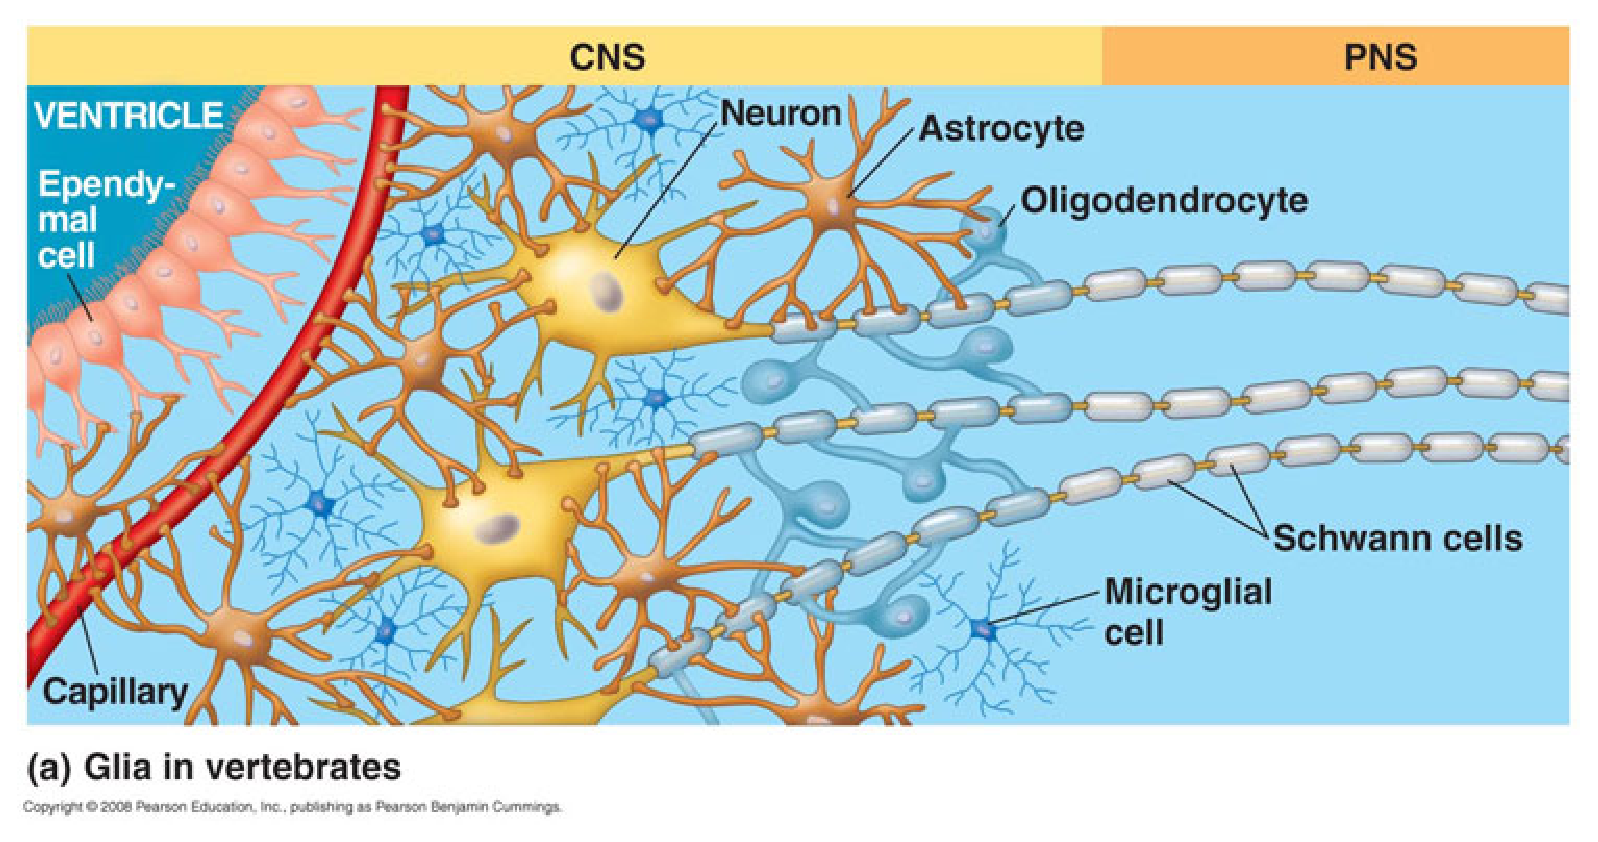
\includegraphics[height=7cm]{./images/glial_cell.eps}}
\caption{Glial cells in the vertebrate}\label{fig:glial_cell}
\end{figure} 

% \section{Central Nervous System (CNS)}
% \label{sec:centr-nerv-syst}

%\section{Models a CNS neuron}
%\label{sec:models-cns-neuron}
\section{*1. G protein-coupled receptors (GPCRs)}
\label{sec:G-protein-coupled-receptor}
\label{sec:GPCR}

{\bf G protein-coupled receptors} (GPCRs) or {\bf G protein-linked receptor}
(GPLRs))  is the family of transmembrane proteins that associates with an
intracellular GTPase called G protein (Sect.\ref{sec:G-protein}).
The name GPCR is given due to the existence of an associated intracellular
trimeric G protein (Sect.\ref{sec:G-protein}) to the receptor.
  
GPCR is made up of a single peptide with a cytosolic region, an extracellular
ligand-binding region and 7 transmembrane (TM) $\alpha$-helices,
Fig.\ref{fig:GPCR}. The TMs are connected via three intracellular and three
extracellular loops. 

The activation of one type of GPCR, upon the binding of a proper agonists, can
lead to several intracellular signal transduction
(Sect.\ref{sec:G_protein_mediated-signaling-pathways}). However, remember that
the time-scale of signaling cascade via GPCR is often slower via ion channel
gating.

Depending upon the type of GPCRs (Sect.\ref{sec:GPCR-classification}) which are
activated depending upon the binding of a wide variety of extracellular signals
such as neurotransmitters and hormones, or even external signals (such as smell,
taste, light). Upon activated, GPCRs are responsible for inter-cellular signal
transduction, such as they control important functions like heart rate and blood
pressure.

GPCRs are the largest class of cell-surface receptors and are used by all
eukaryotic organisms, including yeast. The human genome encodes about 800
different GPCRs (which accounts for 3\% of human encoding genome), with about
150 of them have still-unknown functions (orphan GPCRs), i.e. no endogenous
ligand has been found.


% Common for GPCRs is that they mediate responses to extracellular signals by
% interacting and activating a trimeric GTP-binding protein (G protein -
% Sect.\ref{sec:G-protein}).

\begin{figure}[hbt]
 \centerline{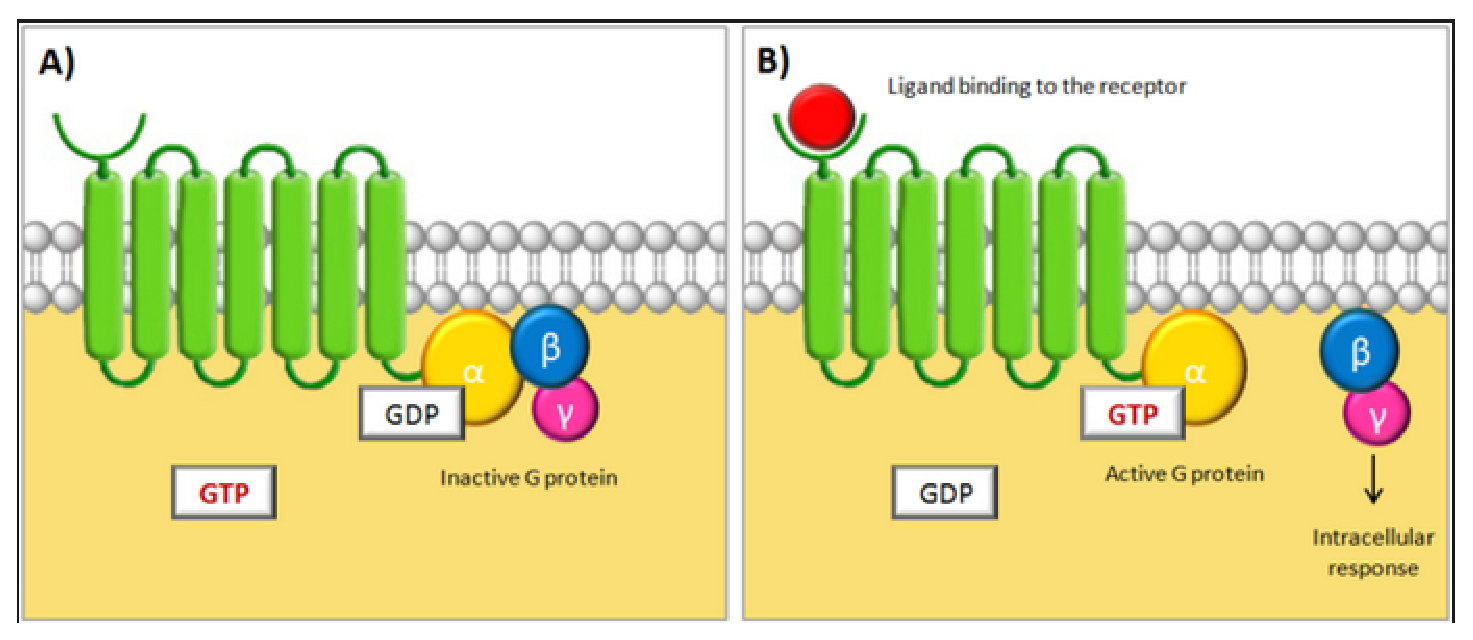
\includegraphics[height=5cm]{./images/GPCR.eps}}
\caption{(A) unbound GPCR; (B) ligand bind to GPCR, which then activate the
bound G protein}
\label{fig:GPCR}
%http://2012.igem.org/Team:Chalmers-Gothenburg/Theory
\end{figure}


\subsection{Classification}
\label{sec:GPCR-classification}

There are different classification schemes have been proposed.
\begin{enumerate}
  \item A,B,C: Sect.\ref{sec:GPCR-classification-1}
  
  \item GRAF : Sect.\ref{sec:GPCR-classification-2}
\end{enumerate}

\subsection{-- class A, class B, class C}
\label{sec:GPCR-classification-1}
\label{sec:GPCR-class-A}
\label{sec:GPCR-class-B}
\label{sec:GPCR-class-C}

\textcolor{red}{\bf A,B,C:} The superfamily was classically divided into three
main classes (A, B, and C) with no detectable shared sequence homology between
classes.

\begin{itemize}

  \item class A GPCR: account for nearly 85\% of genes encoding GPCRs
  
  \item class B GPCR:
  
  \item class C GPCR: include metabotropic glutamate receptors
  (Sect.\ref{sec:mGluR}), and several additional receptors such as extracellular
  calcium-sensing receptors (CaSR, orphan-receptors GPRC6A -
  Sect.\ref{sec:CaSR}), the gamma-amino-butyric acid (GABA) type B receptors
  (GABA$_B$ receptor 1 and GABA$_B$ receptor 2) - Sect.\ref{sec:GABAB-receptor},
  and the vomeronasal type-2 receptors - Sect.\ref{sec:Vomeronasal-receptor}.
  

\end{itemize}

\subsection{-- GRAFS (Glutamate, Rhodopsin, Adhesion, Frizzled/Taste2,
Secretin)}
\label{sec:GPCR-classification-2}
\label{sec:GPCR-GRAFS}

\textcolor{red}{\bf GRAFS}: More recently, an alternative classification system
called GRAFS (Glutamate, Rhodopsin, Adhesion, Frizzled/Taste2, Secretin) has
been proposed with 6 classes based on  sequence homology and functional
similarity
\begin{enumerate}
  \item class 3: Metabotropic glutamate/pheromone
  
  \item class 1: Rhodopsin-like (the largest group of GPCR - Sect.\ref{sec:rhodopsin-like-GPCR})

  \item class 4: Fungal mating pheromone receptors)
  \item class 5: Cyclic AMP receptors
  \item class 6: Frizzled/Smoothened
  \item class 2: Secretin receptor family
\end{enumerate}
\url{http://en.wikipedia.org/wiki/G_protein-coupled_receptor#Classification}

% Each GPCR binds to and is activated by a specific ligand

\textcolor{red}{\bf Ligand-based}: Depending on the ligand, GPCRs
are divided into classes
\begin{enumerate}
  \item Glutamate - Sect.\ref{sec:mGluR}
  \item GABA$_B$ - Sect.\ref{sec:GABA_receptors}
  \item Dopamine - Sect.\ref{sec:dopamine_receptors}
  \item NE, Epi - Sect.
  \item Histamine - Sect.\ref{sec:histamine-receptors}
  \item Serotonin - Sect.\ref{sec:serotonin-receptors}
  \item Purines
  \item Muscarinic
\end{enumerate}
(Sect.\ref{sec:GPCR_ligands}) outside the cells. An important family of ligand
is catecholamine.
\url{http://www.ncbi.nlm.nih.gov/books/NBK10802/figure/A501/?report=objectonly}

Members of GPCR family
\begin{enumerate}
  \item LH/CG receptor (Luteinizing hormone receptor):
  Sect.\ref{sec:LH/CG_receptor} 
  
  \item Cannabinoid receptors - Sect.\ref{sec:cannabinoid-receptors}
\end{enumerate}



\textcolor{red}{IMPORTANT}: Catecholamine (Sect.\ref{sec:Catecholamines})
function as neurotransmitters and hormones within the body. There are three
subtypes of catecholamine, and depending on which one activates GPCR,
the GPCR is classified into 2 types
\begin{itemize}
  \item Adrenergic Receptor - Sect.\ref{sec:adrenergic_receptor}
  \item Dopamine Receptor - Sect.\ref{sec:dopamine_receptors}
\end{itemize}

The ligand-bound GPCR activates G protein (Sect.\ref{sec:G-protein}).
There are different subtypes of G proteins (Gi, G$_{io}$ (Gi/Go), Gs, Gq11,
\ldots). Most receptors are able to activate more than one G protein subtype.
Once a G protein subtype is activated, it triggers a particular intracellular
signal transduction pathways. There are 2 main signal transduction pathways
involved by GPCR
\begin{enumerate}
  \item cAMP signal pathways - Sect.\ref{sec:cAMP-dependent_pathway}
  \item phosphatidylinositol signal pathway - Sect.\ref{sec:phosphatidylinositol-signal-pathway}
\end{enumerate}

\begin{mdframed}
A GPCR involves in many diseases, 
such as diabetes, blindness, allergies, depression, cardiovascular defects, and
certain forms of cancer. As a matter of fact, they are the target of
approximately 30-40\% of all modern medicinal drugs.
\url{http://en.wikipedia.org/wiki/G_protein} 
\end{mdframed}

\subsection{TACR1 (NK1R, SPR)}
\label{sec:TACR1}
\label{sec:NK1R}

The tachykinin receptor 1 (TACR1) also known as neurokinin 1 receptor (NK1R) or
substance P receptor (SPR - Sect.\ref{sec:tachykinin-receptor}) is a GPCR
(Sect.\ref{sec:GPCR}) found in CNS (Sect.\ref{chap:CNS}) and PNS (Chap.\ref{chap:periph-nerv-syst}).
TACR1 consists of 407 amino acid residues, and it has a molecular weight of
58.000

The endogenous ligand for TACR1 is substance P (Sect.\ref{sec:tachykinin}) whose
binding has been associated with the transmission of stress signals and pain,
the contraction of smooth muscles and inflammation.

\subsection{tachykinin: substance P}
\label{sec:tachykinin}
\label{sec:subtance-P}
\label{sec:tachykinin-receptor}

Substance P is a neuropeptide belongs to the {\bf tachykinin} family. 
Subtance P binds to all three of the tachykinin receptors, but it binds most
strongly to the NK1 receptor (Sect.\ref{sec:NK1R}).

Tachykinin receptors are those having 7TM, 3 extracellular loops, 3
intracellular loops, and an amino-terminus and a cytoplasmic carboxy-terminus.
The loops have functional sites, including 
\begin{itemize}
  \item two cysteines amino acids for a disulfide bridge, 
  
  \item Asp-Arg-Tyr, which is
  responsible for association with arrestin and, 
  
  \item Lys/Arg-Lys/Arg-X-X-Lys/Arg, which interacts with G-proteins
  
\end{itemize}

When NK1 receptors are stimulated, they can generate various second messengers.
\begin{enumerate}
  \item trigger phosphotidyl inositol (Sect.\ref{sec:phosphatidylinositol}) via
  PLC (Sect.\ref{sec:PLC}), leading to calcium mobilization  from both intra-
  and extracellular sources.
  
  
  \item phospholipase A2 (PLA2): leading to mobilization of arachidonic acid
  (Sect.\ref{sec:arachidonic-acids})
  
  \item stimulate AC (Sect.\ref{sec:AC_adenylyl_cyclase}): increase cAMP
\end{enumerate}

Example of tachykinin receptors:
\begin{enumerate}
  \item TACR1 (NK1R) - Sect.\ref{sec:TACR1}
\end{enumerate}

The two small peptides, somatostatin and substance P, were present in small
neuronal cell bodies in spinal ganglia, in fibers in the dorsal horn of the
spinal cord and in fibers in the intestinal wall.
However, somatostatin (or somatostatin-like immunoreactivity) and substance P
(or substance P-like immunoreactivity) are present in different sensory cells
(Sect.\ref{sec:sensory_neuron}).

Subtance P (SP) is synthesized by neurons and transported to synaptic vesicles;
the release of SP is accomplished through the depolarizing action of
calcium-dependent mechanisms.


\section{ -- LH/CG receptor}
\label{sec:LH/CG_receptor}

Names: Luteinizing hormone/choriogonadotropin receptor (LH/CG receptor)
or lutropin/choriogonadotropin receptor (LCGR) or luteinizing hormone receptor
(LHR)

These receptors are activated upon binding of luteinizing hormone (LH) and
chorionic gonadotropins (such as hCG in humans) and represents a G
protein-coupled receptor (GPCR). Its activation is necessary for the hormonal
functioning during reproduction. Example: upon binding of LH to the external
part of the receptor, a transduction signal (via receptor shifts conformation)
activate the G protein bound to the internal side, and the detached G protein
subsequently activate cAMP system (Sect.\ref{sec:cAMP-dependent_pathway}).

These receptors are found predominantly in fetal organs and in fallopian and
uterine tissues in women. It can also be found in regions of the adult brain
such as hippocampus, hypothalamus and brain stem.
\url{http://2012.igem.org/Team:Chalmers-Gothenburg/Theory}

\section[ -- Adrenergic receptor (alpha, beta)]{ -- Adrenergic receptor
($\alpha$, $\beta$)}
\label{sec:adrenergic_receptor}

Adrenergic receptors (AR) is a class of GPCR (Sect.\ref{sec:GPCR}) that is
activated by epinephrine and norepinephrine (Sect.\ref{sec:Catecholamines}).
Some can also be modulated by dopamine (Sect.\ref{sec:dopamine}).

The binding of epinephrine and norepinephrine to the receptor will generally
stimulate the sympathetic nervous system (Sect.\ref{sec:sympathetic_nervous
system}).

There are two main groups of AR
\begin{itemize}
  \item $\alpha$-AR - Sect.\ref{sec:alpha-adrenergic-receptor}
   
  \item $\beta$-AR - Sect.\ref{sec:beta-adrenergic-receptor}
\end{itemize}
%\textcolor{red}{We will focus on beta-AR only, as the alpha-AR regulates the
%vasconstrictor (the blood vessel)}.
 
\subsection{$\alpha$-AR}
\label{sec:alpha-adrenergic-receptor}

$\alpha$-adrenergic receptors (AR) have 2 major types:
\begin{enumerate}
  \item $\alpha_1$ AR (Sect.\ref{sec:alpha-1-adrenergic-receptor}): link to
  G$_\alpha$q protein (Sect.\ref{sec:Gq/11-protein}).
  
  
  \item $\alpha_2$ AR (Sect.\ref{sec:alpha-2-adrenergic-receptor}): link to
  G$_\alpha$i protein (Sect.\ref{sec:Gi-protein})
\end{enumerate}
Both epinephrine and norepinephrine activates both the $\alpha_1$ and $\alpha_2$
receptors; yet compared to adrenaline, noradrenaline has a higher affinity for
$\alpha_1$-AR.

\subsection{-- $\alpha$-1 AR (1A, 1B, 1D)}
\label{sec:alpha-1-adrenergic-receptor}

The $\alpha-1$ AR type has 3 subtypes: $\alpha_{1A}, \alpha_{1B}, \alpha_{1D}$.
(NOTE: There was so-called $\alpha_{1C}$ but then later it was identified as
the same as $\alpha_{1A}$; and to avoid confusing, that name is removed without
shifting $\alpha_{1D}$).
 

{\bf $\alpha_1$ AR}: mainly mediate smooth muscle contraction via
Gq$\alpha$ (while $\beta_2$-AR induces relaxing via Gi$\alpha$).
\begin{itemize}
  \item Gq protein activate PLC, i.e. leading to rise in calcium via DAG and IP3
\end{itemize}

\begin{itemize}
  \item \textcolor{red}{vascular smooth muscle}: Associated with vascular smooth
  muscle are a large number of $\alpha_1$ receptors relative to beta2 receptors. 

$\alpha_1$-AR mediates vasconstrictor actions of catecholamines (i.e. the
activation of these AR by either drugs or SNS (Sect.\ref{sec:sympathetic_nervous
system}) narrowing the blood vessels resulting from the contraction of the
muscular wall of the vessels and thus increasing blood pressure) \footnote{The
opposite process of vascontriction is vasodilation, i.e. widening the blood
vessels}.

  \item \textcolor{red}{neuronal}: 
  
  Activation of $\alpha_1$-AR produces (1)  anorexia and (2) partially mediates
  the efficacy of appetite suppressants like phenylpropanolamine and amphetamine in
  the treatment of obesity; 
  
  Activation of $\alpha_1$-AR by norepinephrine decrease cellular excitability in all
  layers of the temporal cortex, including the primary auditory cortex, via
  by inhibiting AMPAR-mediated current \citep{dinh2009}
  
\end{itemize}


\subsection{-- $\alpha$-2 AR}
\label{sec:alpha-2-adrenergic-receptor}

The $\alpha-2$ AR type has 3 subtypes: $\alpha_{1A}, \alpha_{1B}, \alpha_{1C}$.

$\alpha-2$ AR is coupled to G$_{i/o}$ protein.
\begin{itemize}
  \item  Gi protein inactivate AC-III (Sect.\ref{sec:AC-III}), which in turns
  reduce cAMP level (Sect.\ref{sec:cAMP})
\end{itemize}

\textcolor{red}{\bf nerve terminal}: $\alpha_2$ AR exist presynaptically
associated with nerve terminals as an autoreceptor. Here, norepinephrine acts at
presynaptic $\alpha_2$ receptors to inhibit its own release of
neurotransmitters.
\url{http://www.uky.edu/~mtp/OBI836AR.html}



\subsection{$\beta$-AR}
\label{sec:beta-adrenergic-receptor}
% \subsection{-- beta-1 adrenergic receptor}
 \label{sec:beta-1-adrenergic-receptor}
% 
% 
% \subsection{-- beta-2 adrenergic receptor}
 \label{sec:beta-2-adrenergic-receptor}

%$\beta$-adrenergic receptors is a type of GPCR (Sect.\ref{sec:GPCR})

$\beta$-adrenergic receptors have 3 subtypes:
\begin{enumerate}
  \item $\beta_1$: link to Gs protein (Sect.\ref{sec:Gs-protein})

Beta-1 adrenergic receptors is expressed predominantly in cardiac tissue.
  
  \item $\beta_2$: link to Gs protein (Sect.\ref{sec:Gs-protein}) and 
  Gi protein (Sect.\ref{sec:Gi-protein}).
  

Unlike $\alpha$-1 AR which induces contraction, $\beta_2$-AR induces relaxing in
smooth muscle.
  
  \item $\beta_3$: link to Gs protein  
\end{enumerate}
Epinephrine activates both the beta1 and beta2-AR. Norepinephrine
activates only the beta1-AR.

As three $\beta$-AR subtypes all link to Gs-coupled receptors.
Gs stimulating activity AC-III (Sect.\ref{sec:AC-III}),
which rise [cAMP] (Sect.\ref{sec:cAMP}) -
Sect.\ref{sec:beta-adrenergic_stimulation}.

\begin{enumerate}
  \item $\beta$-AR stimulation coupled to Gs-protein released
  (Sect.\ref{sec:Gs-protein})
  
  \item Gs-protein activate AC-III  (Sect.\ref{sec:AC-III})
  and also Gs-protein directly activates the Ca2+ channel.
  
  \item Activation of AC-III catalyze the conversion from ATP to cAMP and pyrophosphate
  
  \item The rise in intracellular cAMP activate PKA (Sect.\ref{sec:PKA})
  
  \item PKA phosphorylates the Ca2+ channel promoting Ca2+ influx, i.e. rise in
  $[\Ca]_i$ and trigger contraction.

In LCC, the increase in $\Ca$ current is the result of an increase in $P_o$ and
channel availability, rather than the elevated unitary current values
\citep{uehara2002, schroder1998}

NOTE: $\beta$-adrenergic receptor stimulation increase LCC opening
probability, while the effect in $\Na$ is controversal.
  
  \item PKA phosphorylates the sarcoplasmic reticulum leading to an increase in Ca2+ uptake and
  release. 
  \begin{itemize}
    \item SERCA via phospholamban (Sect.\ref{sec:PLN_SERCA})
  
    \item RyR
  \end{itemize}
  
  \item PKA phosphorylates troponin changing its calcium binding kinetics, i.e.
  increase contractile force and heart rate
 
\end{enumerate}


\section{ -- Dopamine receptors (DR)}
\label{sec:dopamine_receptors}

Dopamine receptors are transmembrane proteins that can bind to dopamine
(Sect.\ref{sec:dopamine}).


All the cloned {\bf dopamine receptors} so far are a class of GPCR
(Sect.\ref{sec:G-protein-coupled-receptor}) with 7-TM regions.
One of the intracellular loops is larger than the rest and it is this loop that
interacts with the G-protein complex (Sect.\ref{sec:G-protein}).

There are at least five subtypes of dopamine receptors, D1, D2, D3, D4, and D5;
with \textcolor{red}{D1 and D2 are the most abundant subtypes}.
D1 and D2 receptor subtypes are found at 10-100 times the levels of the D3-5
subtypes. 

There is also some evidence that suggests the existence of possible D6 and D7
dopamine receptors, but such receptors have not been conclusively identified.
Based on G-protein coupling and the length of the 3rd cytoplasmic loop
and the carboxyl tail, they are grouped into two major classes (Review:
\citep{emilien1999}).
\begin{enumerate}
  \item D1-like subtype - Sect.\ref{sec:D1-like-receptors}
  
  \item D2-like subtype - Sect.\ref{sec:D2-like-receptors}
\end{enumerate}

\begin{mdframed}

As GPCRs are essentially slow that mainly functionally modulate other receptor
systems and/or ion channels.  Hence, with a few exceptions, activation of
dopamine receptors {\it per se} in the forebrain does not induce large
postsynaptic currents that - at least in vitro - can be measured
electrophysiologically (Yang and Seamans, 1996). Rather, activation of DA
receptors modulates, via intracellular cascades, a set of biophysical properties
of the synapses and the postsynaptic neurons that changes their information
processing properties. 
\end{mdframed}





% 
% The action of dopamine (Sect.\ref{sec:dopamine}) in the brain is mediated by
% different dopamine receptor (DA receptor) subtypes. 

\subsection{Theurapeutic role}

D2-receptors have been implicated in the pathophysiology of schizophrenia and
PD.  However, the improved therapy of both disorders may lie in developing drugs
that target a particular subtype of DA receptors.
\begin{itemize}
  \item  In schizophrenia: DA receptor {\bf antagonists} or neuroleptics
such as haloperidol block hallucinations and delusions
that occur at various stages of schizophrenia, while on the
other hand, DA receptor agonists such as bromocriptine alleviate
the hypokinesia of PD. 
  
  \item In PD: DA {\bf agonists} could prevent or reduce the postsynaptic
  changes that underlie fluctuations of motor symptoms and dyskinesias that
  often accompany sustained levodopa (Ldopa)  treatment and, therefore, could be
  used either as early  adjunct therapy with L-dopa or initially as a DA
  monotherapy 
\end{itemize}

DA hydrochloride, administered only intravenously, is
widely used in the treatment of various shock states
(Sect.\ref{sec:dopamine-theurapeutic-role}).


\subsection{D1-like receptors: D1R (human) or D1$_A$R (rat), D5R (human) or
D1$_B$R (rat)}
\label{sec:D1-like-receptors}


D1-like family belongs to DA receptors (Sect.\ref{sec:dopamine_receptors}) with
two subtypes: \textcolor{red}{D1$_A$ and D1$_B$ in rats. D1$_B$ is also known as
D5 in humans and D1$_A$ is D1 receptor in human}.
D1-like family has a longer 3rd cytoplasmic loop and carboxyl tail: D1 and D5.

NOTE: D1 and D2 receptor subtypes are found at 10-100 times the levels of the
D3-5 subtypes.   

Although human D1-like receptors share a highdegree of amino acid sequence
identity, there are variations in regional, cellular and subcellular
distributions of D1R and D5R, as well as distinctive ligand binding, G protein
coupling and signaling properties (Tiberi and Caron 1994;Bergson et al. 1995;
Missale et al. 1998; Ciliax et al. 2000;Huang et al. 2001; Neve et al. 2004;
Paspalas and Goldman-Rakic 2004). \textcolor{red}{It suggests that D1R and D5R
are not functionally redundant, but may play distinct regulatory roles in
synaptic transmission and endocrine functions}.
However, understanding this distinct role is challenging due to  the lack of
subtype-specific agonists and antagonists for D1-like receptors.

\begin{itemize}
  \item D1: D1 subtype is the most abundant DR in CNS (in rodent and monkey PFC,
  it is 10-fold higher than other subtypes). It also modulate D2-subtype-mediated events.
 
  \item D5 subtype has about 10x higher affinity for dopamine than D1 subtype.  
\end{itemize}

{\it D1 subtype shows monophasic dose-dependent accumulation of cAMP in response
to dopamine; while D5 subtype shows biphasic accumulation under the same
condition}, suggesting D5 subtype may use a different cascading system than D1
subtype.
\begin{enumerate}
  \item  D1 subtype involve in the formation of LTP while D5 subtype involve
in the formation of LTD in rodent striatum \citep{}
  
  \item 
\end{enumerate}

\subsection{**** D1R}
\label{sec:D1R}

As a GPCR, the activation of D1-like family coupled with the release {\bf
(G$\alpha$s-, Gq- or GOlf-)} protein  (Sect.\ref{sec:Gs-protein},
 Sect.\ref{sec:Gq/11-protein}).   D1 receptors have been classically
defined as being linked to the stimulation of adenylyl cyclase activity (see
below).
 
The released $G_s\alpha$-GTP 
\begin{enumerate}
  
  \item   binds to and activates  adenylyl cyclase type V
  (Sect.\ref{sec:AC-IIIa-type-V}) that subsequently catalyzes the conversion from ATP to
  cAMP (Sect.\ref{sec:cAMP}), i.e. increase  intracellular [cAMP] which enables
  cAMP to involve into multiple signaling cascades
  (Sect.\ref{sec:cAMP-dependent_pathway}).
  
  \item [not well-known] directly enhance NMDAR currents, via L-type Vm-gated
  $\Ca$ channel (Liu et al., 2004)
  
  \item reduce $\Na$ channel (e.g. Nav1.1) conductivity
  \item inhibit N-type Vm-gated $\Ca$ channel (Kisilevsky et al., 2008,
  Surmeier and Kitai, 1993)
  
\end{enumerate}
Such actions make D1-R consistents with the classical notion as 'excitatory'
 


 
\subsection{**** D5R}
\label{sec:D5R}

Activation of D5 subtype is shown to 
\begin{itemize}

  \item promote expression of BDNF (brain-derived
neurotrophic factor)  which may link to LTP plasticity
(Sect.\ref{sec:BDNF-mediate-LTP})

However, in D1-D2 MSN, Dopamine-induced BDNF does not require D5 receptor
(Hasbi et al., 2009).-Sect.\ref{sec:D1-D2-heteromer-MSN}

  \item increase phosphorylation of protein kinase B in rat and mice prefrontal
  cortex neurons 
\end{itemize}


\subsection{D2-like (D2S, D2Lh, D2L, D3, D4)}
\label{sec:D2-like-receptors}

D2-like family has a shorter 3rd cytoplasmic loop and carboxyl tail; which
\textcolor{red}{comprises D2S-, D2L-, D3-, and D4-receptor subtypes}.
\begin{itemize}
  \item  D2Lh- (or D2lh-) is the cannonical long-form of the D2-receptor, and is
  the post-synaptic receptor
  
  \item D2S- (or D2s-) is the short form (D2Sh) and is pre-synaptic and
  functions as an auto-receptor that regulates the levels of dopamine in the
  synaptic cleft.
  
  Agonism of D2sh receptors inhibits dopamine release; antagonism increases
  dopaminergic release.
  
  \item A third D2(Longer) form differs from the canonical sequence where 270V
  is replaced by VVQ
\end{itemize}


Unlike D1-receptors, activation of D2 receptors results in various responses,
including inhibition of adenylyl cyclase activity
(Sect.\ref{sec:adenylyl-cyclase-classIII}), inhibition of phosphatidylinositol
turnover (Sect.\ref{sec:PIP2}), increase in K+ channel activity, and inhibition
of Ca2+ mobilization.
  
The activation of D2-like family coupled with Gi/o protein
(Sect.\ref{sec:Gi/o-protein}), which release  
\begin{enumerate}

  \item G$\alpha_i$ subunit: directly inhibits the formation of cAMP by
  inhibiting the AC enzyme (Stoof and Kebabian, 1994).

  \item G$\beta\gamma$ subunit: 
  \begin{itemize}
    \item reduce Cav2 $\Ca$ channel openings 
    
    \item stimulate phospholipase 	C$\beta$ isoforms (Sect.\ref{sec:PLC-beta})
    \item generate DAG (Sect.\ref{sec:DAG})
    \item generate PKC (Sect.\ref{sec:PKC})
    \item mobilization of intracellular $\Ca$ store (Hernandez-Lopez et al.,
    2000, Nishi et al., 1997)
  \end{itemize} 

  \item other roles:
  \begin{itemize}
     \item transactivating tyrosine kinase (Kotecha et al., 2002)
     
     \item negatively modulate Cav1.3 $\Ca$ channel through calcineurin-dependent
    mechanism (Olson et al., 2005)
    
     $\rightarrow$ reduce NMDAR currents
    in striatum (Hernandez-Echeagary et al., 2004)
    
    \item [unclear from pre- or post-synaptic D2R] diminish presynaptic release
    
    \item reduce opening of Vm-gated $\Na$ channel, via PKC-mediated enhancement
    of slow inactivation (Surmeier and Kitai, 1993)
    \item promote opening of $\K$ channel (Greif et al., 1995)
  \end{itemize}
\end{enumerate}

The effect on plasticity (LTP, LTD) is complex and depends on (1) receptor
subtypes, (2) concentration level, (3) types of plasticity (LTP or LTD).
Evidences of non-linear doses effect on plasticity have been found 
\begin{itemize}
  \item  using D2/D3 agonist {\bf ropinirole}: reveal non-linear dose effect
  only on facilitatory not inhibitory plasticity in humans.
  
  NOTE: ropinirole predominantly activates D3 rather than D2 receptors.
  
  \item in rat studies: facilitation by D2 receptor, but inhibition by D3
  receptor activation 
  
  NOTE: with neurotensin gene expression in rat, D2 receptors has negative
  effect, while D3 has positive one.
  
  \item 
\end{itemize}

\subsection{Agonist}
\label{sec:D2-receptor-agonist}
\label{sec:D1-receptor-agonist}

\begin{enumerate}
  \item Dopamine (DA) : natural agonist to D1R and D2R
  
  
  \item SKF 8359: D1-D2 heteromer agonist
  
SK 8350 has a  higher maximal peak effect for dopamine (Emax = 0.5 versus 0.35
for SKF 83959); but equivalent EC50 values (170 nM for dopamine and 152 nM for
SKF 83959).  (Hasbi et al. 2009)
 
As SKF 83822 also exclusively activates the cAMP pathway. To ensure ER $\Ca$
release is not via this pathway, they block cAMP and showed no significant
effect on intracellular calcium release, suggesting the noninvolvement of this
pathway in $\Ca$ release (Hasbi et al., 2009).

  \item SKF 38393 hydrobromide : D1-receptor agonist 

  \item [11C]raclopride : D2-specific agonist 
  
  \item bromocriptine: D2-specific agonist

  \item Quinpirole (100 nM): a D2-specific agonist

The response to quinpirole (100 nM) was blocked by the D2 receptor antagonist
(-)-sulpiride (1 pM) (Fig. 2B, n = 5), suggesting that the modulation was
mediated by D2-like receptors.

Quinpirole at concentrations < 10 $\mu$M, showed no effect, but at higher
concentrations ($\ge$ 10 $\mu$M) triggered calcium mobilization.
This occurs via Gq activation leading to PLC,IP3, and ER $\Ca$ release (Hasbi
et al., 2009).

Such quinpirole concentrations are far higher than its affinity constant (Kd
1.5-2.2 nM) for D2 receptor in rat striatal membranes (21) and would not be
specific for D2 receptors. However, 1-100 nM quinpirole used concomitantly with
equivalent concentrations of SKF 83959 showed an effect one to two times greater
than the effect of SKF 83959 alone, indicating a synergistic effect of D1 and D2
receptor activation.


\end{enumerate}


\subsection{Antagonist}
\label{sec:DA-receptor-antagonist}

\begin{enumerate}
  \item  SCH 23390, a D1-specific antagonist, and 
  
  \item raclopride, a D2-specific antagonist,
  
  \item Sulpiride is a selective antagonist at dopamine D2 and D3 receptor

  
\url{https://en.wikipedia.org/wiki/Sulpiride}
\end{enumerate}


In schizophrenia (Sect.\ref{sec:schizophrenia})
\begin{enumerate}
  \item {\bf Chlorpromazine}:  (Sect.\ref{sec:chlorpromazine})
  
  \item 
\end{enumerate}


\section{ -- Histamine receptors}
\label{sec:histamine-receptors}

The histamine receptors are a class of G protein-coupled receptors
(Sect.\ref{sec:GPCR-in-neurons}) with histamine as their endogenous ligand.

There are 4 known histamine receptors
\begin{enumerate}
  \item H1 receptor: Gq-protein (Sect.\ref{sec:Gq/11-protein})
  \item H2 receptor: Gs-protein (Sect.\ref{sec:Gs-protein})
  \item H3 receptor: Gi-protein (Sect.\ref{sec:Gi-protein})
  
  \item H4 receptor: Gi-protein
\end{enumerate}

 \textcolor{red}{H1 and H2 are quite different from H3 and H4 in their
 activities}. H1 causes an increase in PIP2 hydrolysis, H2 stimulates gastric
 acid secretion, and H3 mediates feedback inhibition of histamine.
 
\section{ -- mGluR: metabotropic glutamate receptors}

Check Sect.\ref{sec:mGluR}.
 
 \section{ -- Vomeronasal receptors (V1, V2, V3)}
 \label{sec:Vomeronasal-receptor}

\section{ -- Muscarinic acetylcholine receptor (mAchR)}

Check Sect.\ref{sec:mAchR}.

\section[ -- GABA-B receptor]{ -- GABA$_\text{B}$ receptor}

Check Sect.\ref{sec:GABAB-receptor}.

\section{ -- Aminergic receptors}
\label{sec:aminergic-receptors}

{\bf Aminergic receptors} is a GPCR, i.e. aminergic GPCR. 

Members \citep{brunskole2011}
\begin{enumerate}
  \item histamine H2 receptor (H2R): 
  
  using histamine H2 (HA (2-(1H-imidazol-4-yl)ethanamine)) as an endogenous
  ligand
  
  \item histamine H4 receptor (H4R) and the 
  
  \item $\beta$2-adrenergic receptor ($\beta$2AR), 
\end{enumerate}
The H2R and $\beta$2AR, also expressed on neutrophil granulocytes, are some of
the best characterized aminergic GPCRs.
Classically, both, the H2R and the $\beta$2AR couple to Gs protein
(Sect.\ref{sec:Gs-protein}). Other evidences suggested
$\beta$2AR can also ``signal'' via Gi proteins (Sect.\ref{sec:Gi/o-protein}), Gq
proteins (Sect.\ref{sec:Gq/11-protein}) and $\beta$-arrestin, triggering
responses distinct from those activated through Gs proteins.


\section{ -- Serotonin receptors (5-HT receptors)}
\label{sec:serotonin-receptors}
%\subsection{5-HT receptor}
\label{sec:5-HT_receptor}

{\bf Serotonin receptors} (5-HT receptors) are family of both GPCR
(Sect.\ref{sec:G-protein-coupled-receptor}) and ligand-gated receptors with the
natural agonist is serotonin (Sect.\ref{sec:serotonin}).



\subsection{Localization}

The serotonin receptors modulate the release of many neurotransmitters,
including glutamate, GABA, dopamine, epinephrine / norepinephrine, and
acetylcholine, as well as many hormones, including oxytocin, prolactin,
vasopressin, cortisol, corticotropin, and substance P
(Sect.\ref{sec:substance-P-like-neuron}), etc.

Despite this broad axon terminal domain of 5-HT neurons, 5-HT terminals
preferentially target motor areas in CNS.
Several recent studies have emphasized a crucial role for the interactions
between serotonergic and dopaminergic systems in voluntary movement control and
the pathophysiology of basal ganglia (Sect.\ref{sec:basal-ganglia}).
Serotonergic terminals (releasing 5-HT serotonin) have been reported to make
synaptic contacts with ({\bf review: Di Matteo et al., 2008}).

\begin{itemize}
  
  \item  both substantia nigra
  dopamine-containing neurons (Sect.\ref{sec:SNpr})
  
NOTE: This region is the greatest input of Serotonin.
 
  \item (location at the target of DA neurons) the basal ganglia (i.e.
  striatum, the globus pallidus and the subthalamus).
\end{itemize}

Many of the 5-HT receptors are found within the basal ganglia and most likely
involved in the modulation of basal ganglia circuitry and in the pathology of
their correlated disorders.
\begin{enumerate}
  \item  {\bf 5-HT1A and 5-HT1B/1D receptor subtypes}: 5-HT1B receptor in
  rat/rodent is equivalent to 5-HT1D in other higher level species (see below).

In a large scale study using autoradiographic data, it showed a lack of 5-HT
receptors in cats, guinea pigs, monkeys and humans, of receptors with a
pharmacological profile similar to that of the rat and mouse 5-HT1B.
It is suggested that 5-HT1D receptor found in these species is the homologue to
5-HT1B in rat. In human, two genes expressing different receptors displaying the
pharmacology of the originally described 5-HT1D receptors: 5-HT1D$\alpha$, and
5-HT1D$\beta$, showed 96\% homology to the cloned rodent 5-HT1B receptor.


DISTRIBUTION:   5-HT(1A) is found mainly in soma and dendrites of pyramidal
cells in layer III and V or cortex, and hippocampal formation
  \begin{itemize}
    \item hippocampal formation: dendrite (mostly along extrasynaptic portions
    of their plasma membrane)
    
 Using immunogold labeling, membrane-associated 5-HT1A receptors could be
 estimated to be at least 30-40 times that in the cytoplasm
    
    \item cortex: -  (e.g. axon  initial segments of layers III and V pyramidal cells)
  \end{itemize}
,  beside a localization on calbindin and paralbumin staining interneurons.
5-HT1A receptors confined to striosomes of the primate striatum characterized by
poor calbindin immunostaining.

There is a dorsoventral gradient of 5-HT1B/1D with higher levels in the ventral as
compared to the dorsal striatum in both rats and human. In rats and mice, it has
intermediate-to-low concentrations of 5-HT1B binding or immunoreactivity sites in the caudate-putamen.
5-HT1B receptor subtype is found on on axon terminals arising from medium spiny
neurons (MSNs) of the ventral striatal regions.

As there is a discrepancy in the distribution pattern of 5-HT1B/1D mRNA and the
expressed protein in the striatum, SN and GP of mouse brain, it is hypothesized 
a presynaptic localization of 5-HT1D receptors in the
latter two areas.

  \item {\bf 5-HT1E receptor subtype}:
  
The presence of 5-HT1E receptor subtype mRNA in both the caudate nucleus and
putamen of primates, showing stronger hybridization signals in monkey brain than
that obtained in human brain.


  \item {\bf 5-HT2A and 5-HT2C receptor subtypes}

Both 5-HT2A receptor subtype and its mRNA have been extensively demonstrated to
be present in the striatum of various mammal species, with 
increasing gradients in the rostrocaudal and mediolateral directions.

5-HT2A receptors showed a somatodendritic localization.
A more prominent localization in dendrites than in cell bodies was found in the
dorsolateral caudateputamen of rat brain, using immunocytochemistry.


Widespread distribution of the 5-HT2C receptor subtype in rat, monkey and human
brains, particularly among the different basal ganglia structures.
Moreover, marked differences have been revealed in the distribution of 5-HT2C
mRNA and its level of expression within the different subregions of the basal
ganglia. In studies in 1990s, the neurons with expressed 5-HT2C are mostly
efferent MSNs, but not cholinergic interneurons. 

However, recent polymerase chain reaction (PCR) evidence instead revealed high
expression of 5-HT2C, 5-HT6 and 5-HT7 mRNAs in cholinergic interneurons (Bonsi
et al., 2007a).

5-HT2C receptors are not differentially expressed on the two major striatal
output pathways (striatonigral and striatopallidal projection neurons), i.e.
with equally found in localization with substance P, dynorphin or enkephalin.
However,  5-HT2C mRNA showed a preferential localization in the patch
compartment areas (Sect.\ref{sec:striosomes-striatum}), suggesting a role for
this receptor in the modulation of striatal projections to the SNc


  \item {\bf 5-HT3 receptor}:
  
5-HT3 receptors have been found in the striatum of different mammals, albeit
higher receptor densities have been found in the human caudate nucleus and
putamen than in the corresponding structures of the rat brain.
Synaptosomes data also show the presence in rat striatum  of functional
presynaptic 5-HT3 receptors, besides the known postsynaptic localization.

  \item {\bf 5-HT4 receptors}:
  
The distribution pattern of the 5-HT4 receptor binding sites in the striatum
matched that observed for its mRNA in all the different species used in binding
and in situ hybridization studies. However, there are species dependent data:
\begin{itemize}
  \item  ventromedial-to-dorsolateral-increasing gradients of labelling
densities have been observed in the rat and mouse brain caudate-putamen
 
Such gradient is less pronounced in the same structure of guinea pig
brain;
 
  \item monkey and human caudate nuclei and putamens showed very high densities
of receptor and mRNA binding sites but no apparent gradient in their
distribution.

\end{itemize}

In rat caudate-putament, it showes somatodendritic localization of 5-HT4
receptors on GABAergic projection neurons and cholinergic/GABAergic interneurons
in this structure. 

5-HT4 receptors are not found in DAergic terminal.

  \item {\bf 5-HT5 receptors}:
  
Only moderate-to-low expression of 5-HT5A receptor protein and mRNA has been
found in the striatum of mouse, rat and human brain.

5-HT5A immunoreactivity was detectable at low levels in MSNs of rat
caudate-putamen.

  \item {\bf 5-HT6 receptors}:
  
As the regional distribution of 5-HT6 receptor generally matched that found for
the 5-HT6 receptor mRNA, it is likely that the former is mainly ocalized on
somas and/or dendrites of neurons.

5-HT6 receptor subtype has been shown to be particularly abundant in this
area of the basal ganglia.

High levels of both protein and mRNA expression have been found in the
caudate-putamen of rat and pig brain, as well as in the caudate
nucleus and putamen of human brain.

In contrast, only low levels of both 5-HT6 receptor protein and mRNA have been
found in the same brain areas of two different strains of mice.

  \item {\bf 5-HT7 receptor}:

5-HT7 receptor subtype has been reported in the striatum of rodents as well as
in the caudate nucleus and putamen of human brain, with a protein distribution
pattern generally matching that of its mRNA.

In addition, some species' differences in receptor densities were reported
between human and rodent brain.

\end{enumerate}


\subsection{Classification: 5-HT1 to 5-HT7}

There are more than 15 cloned types of HT receptors; and they are classified
into seven distinct families of 5-HT receptors: 5-HT$_1$ to 5-HT$_7$.

\textcolor{red}{ONLY 5-HT$_3$ is ligand-gated ion channels
(Sect.\ref{sec:5-HT3-receptor}); all other 5-HT receptors are G-protein-coupled
receptors}.

%TODO : update information about 5-HT's role in mGlur and PLC

\begin{enumerate}

  \item 5-HT$_1$ receptor: link to Gi/o protein (Sect.\ref{sec:Gi/o-protein})
  which decrease cAMP production (Sect.\ref{sec:cAMP-dependent_pathway})
  
  5-HT(1A,1B,1D,1E,1F): there is no 5-HT(1C) as it as later redesignated as
  5-HT(2C). NOTE: 5-HT1D in human/cat/guinea pigs/monkey is the homology to
  5-HT1B in rat/rodent.  So, the nomenclature is revised and they are often
  written as 5-HT1B/1D receptor.
 
  \item 5-HT$_2$ receptor: link to Gq/11 protein (Sect.\ref{sec:Gq/11-protein})
  which increase level of IP3 and DAG (Sect.\ref{sec:GPCR-PLC-IP3-DAG-pathway}) 
  
  5-HT(2A,2B,2C)
  
  DISTRIBUTION: 5-HT(2A) is restricted to layer I throughout the cortex (a
  triggered zone in the distal apical dendrite) in addition to a thin band in
  layer V; a high density of postsynaptic 5-HT(2A) is also found in nodal point
  where the branches of apical dendritic tuft converge; and found on dendrites
  of interneurons.
  
  
  \item 5-HT$_4$ receptor: link to Gs protein (Sect.\ref{sec:Gs-protein}),
  which increase cAMP production (Sect.\ref{sec:cAMP-dependent_pathway}) 
  
  
  may be involved in memory and learning, and they are markedly decreased in
  patients with Alzheimer's disease
  
  \item 5-HT$_5$ receptor: link to Gi/o protein (Sect.\ref{sec:Gi/o-protein})
  
  5-HT(5A, 5B)
  
  the pharmacological function of 5-HT5 receptors is currently unknown
  
  \item 5-HT$_6$ receptor: link to Gs protein
  
  \item 5-HT$_7$  receptor: link to Gs protein 
\end{enumerate}
\url{https://www.acnp.org/g4/GN401000039/Ch039.html}

\subsection{Agonist}

\begin{enumerate}
  
  \item Tetrodotoxin (TTX): 
  
  
  1$\muM$ TTX increases 5-HT release 55.2 $\pm$ 9 ng/cm2/30 min.
  This changes significantly increase upon the apply of 50$\muM$ methacholine -
  a muscarinic agonist, i.e. to 79.3 $\pm$ 9 ng/cm2/30 min.
  It suggested that a muscarinic receptor at or near the enterochromaffin
  cells mediates mucosal 5-HT release. 
  
  
  \item CP 93129: selective 5-H1 (1B) receptor agonist, about
  150x and 200x selectivity over the closely related 5-HT1D and 5-HT1A
  receptors.
  
  \item 
\end{enumerate}

\subsection{Antagonists}

5-HT receptors blockers:
\begin{itemize}
  \item M100907: 5-HT (2A) receptor antagonist
  
  \item  SR46349-B: 5-HT (2A/2C) receptor antagonist
  
  can enhance dopamine (DA) release in rat medial prefrontal cortex (mPFC), an
  effect which has been postulated to be of value to improve cognition and negative symptoms. T
  

  \item Chlorpromazine: 
  
  
\end{itemize}

\subsection{ -- TAAR1 (intracellular receptor)}
\label{sec:TAAR1}

Trace amine-assorted receptor 1 (TAAR1) is a recently discovered GPCR
in 2001 (Sect.\ref{sec:GPCR-in-neurons}), encoded by TAAR1 gene. 

TAAR1 is one of six functional trace amine-associated receptors in humans, which
are so named for their ability to bind low-concentration, endogenous monoamines
called trace amines or closely related compounds.

They are found located in several peripheral organs and circulating
lymphocytes, as well as in astrocytes and within the presynaptic plasma membrane
of monoamine neurons in CNS (Sect.\ref{sec:monoamine-neuron}).
TAAR1 plays a significant role in regulating neurotransmission in dopamine,
norepinephrine, and serotonin neurons in the CNS.

Human TAAR1 is an \textcolor{red}{intracellular receptor} expressed within the
presynaptic terminal of monoamine neurons.  TAAR1 ligands must enter the
presynaptic neuron through a membrane transport protein, or be able to diffuse
across the presynaptic membrane in order to reach the receptor.
\begin{enumerate}
  \item Hypothesis that TAAR1 inhibit the dopamine reuptake
  
  Synaptic dopamine binds to the dopamine autoreceptor, which activates the DAT
  (dopamine transporter). Dopamine enters the presynaptic cells and binds to
  TAAR1
  
  
  \item 
\end{enumerate}

There are two types
\begin{enumerate}
  \item amine-activated Gs-coupled protein
  
  \item amine-activated Gq-coupled protein
\end{enumerate}



\subsection{-- Rhodopsin-like GPCR}
\label{sec:rhodopsin-like-GPCR}

This is the largest group of GPCR. Its members are
\begin{enumerate}
  \item Muscarinic receptors (Sect.\ref{sec:muscarinic-acetylcholine-receptor})
  \item Bradykinin reeptor (Sect.\ref{sec:Bradykinin-receptor})
\end{enumerate}

\section{-- Adenosine receptor (P1 receptor)}
\label{sec:adenosine-receptor}
\label{sec:P1-receptor}


The adenosine receptors (or P1 receptors) are %a class of purinergic GPCR
class A GPCR (Sect.\ref{sec:GPCR}) with adenosine as endogenous ligand. There
are 4 types of adenosine receptors in human, each encoded by a different gene and have
different functions (though with some overlaps)

Adenosine receptors were first identified in the 1970s (van Calker et al.,
1979), and then later was subclassified into the following subfamilies
\begin{enumerate}
  
  \item A2A receptor (Gs - Sect.\ref{sec:A2A-receptor}) -
  Sect.\ref{sec:Gs-protein}: found  in neurons of CNS, stimulate cAMP 
  via activation of AC-III (Sect.\ref{sec:AC-III})
  
Subclassification of A2-adenosine receptors was introduced later to account for
the receptor that required low concentrations of adenosine and adenosine
analogues for the stimulation of AC (Bruns et al., 1986).
  
  \item A2B receptor (Gs): a closed relative to A2A receptor


  \item A1 receptor (Gi/o) - Sect.\ref{sec:Gi/o-protein}:,
  interact with pertussis-toxin-sensitive G proteins of the Gi/o and thus
  inhibit cAMP

A1A and A3A receptors are two more distant relatives of A2A receptors.

  \item A3 receptor (Gi/o):
  interact with pertussis-toxin-sensitive G proteins of the Gi/o
  
\end{enumerate}

\subsection{Adenosine A1A receptor}
\label{sec:A1A-receptor}
\label{sec:Adenosine-A1A-receptor}

A1 receptor is a class A GPCR (Sect.\ref{sec:GPCR-class-A}) with adenosine as
endogenous ligand (Sect.\ref{sec:adenosine}) binding to Gi1/2/3 or Go protein.

\begin{itemize}
  \item activation of Gi1/2/3 causes inhibition of AC
  (Sect.\ref{sec:adenylyl-cyclase-classIII}), and therefore decrease cAMP
  concentration
  
  \item 
\end{itemize}

NOTE: 
\begin{enumerate}
  \item in muscle (heart): A1 receptors present in smooth muscle throughout the
  vascular system.
  
Regulating myocardial oxygen consumption and coronary blood flow: activatioin of
A1 receptors decrease the conduction of electrical impulses and suppressing
pacemaker cell function, resulting in a decrease in heart rate.
  
  \item in brain:
  A1 receptors are implicated in sleep promotion by inhibiting wake-promoting
  cholinergic neurons in the basal forebrain (Sect.\ref{sec:basal-forebrain}).
  
\end{enumerate}



\subsection{Adenosine A2A receptors}
\label{sec:A2A-receptor}
\label{sec:Adenosine-A2A-receptor}

Adenosine A2A receptor is a member of adenosine receptor
(Sect.\ref{sec:adenosine-receptor}), i.e. it uses adenosine as the preferred
endogenous agonist and preferentially interacts with the G(s) and G(olf) family
of G proteins to increase intracellular cAMP levels
(Sect.\ref{sec:cAMP-dependent_pathway}).
\url{https://www.ncbi.nlm.nih.gov/gene/135}


It plays an important role in many biological functions, such as cardiac
rhythm and circulation, cerebral and renal blood flow, immune function, pain
regulation, and sleep. It has been implicated in pathophysiological conditions
such as inflammatory diseases and neurodegenerative disorders. Alternative
splicing results in multiple transcript variants

A2A receptor is highly enriched in striatopallidal neurons and can form
functional heteromeric complexes with other G-protein-coupled receptors,
including dopamine D2 (Sect.\ref{sec:A2A-receptor-D2-receptor-heteromer}),
metabotropic glutamate mGlu5
(Sect.\ref{sec:A2A-receptor-mGluR5-receptor-heteromer}) and adenosine A1
receptors (Sect.\ref{sec:A1A-receptor}).

\subsection{--theurapeutic role}

Because of A2A-D2-complex, the adenosine A2A receptor has emerged as an
attractive non-dopaminergic target in the pursuit of improved therapy for
Parkinson's disease (PD) - Sect.\ref{sec:Parkinson-disease}.

Adenosine A2A receptor (A2AR) is upregulated in the human forebrain of aged and
Alzheimer's disease (AD) patients.
Age-related disorders are associated with downregulation of glucocorticoid
receptors (GR) in the hippocampus (Sect.\ref{sec:glucocorticoid-receptor}), and
subsequent desensitization of the regulatory feedback to the hypothalamus.

Batalha et al. (2016) showed that anti-A2AR therapy reverts age-like memory
deficits, by reestablishment of the hypothalamic-pituitary-adrenal (HPA) axis
feedback and corticosterone circadian levels. A2AR is a major regulator of GR
function and that this functional interconnection may be a trigger to
age-related memory deficits.
% https://www.ncbi.nlm.nih.gov/pubmed/27510168



\subsection{-- Agonist / Antagonist}

{\bf Agonist}
\begin{enumerate}
  \item CGS 21860
\end{enumerate}

{\bf Antagonist}
\begin{enumerate}
  \item SCH 58261 (100 nM): 
  
  \item 1,3-[3H]Dipropyl-8-cyclopentylxanthine ([3H]DPCPX): selective A1A
  receptor antagonist
  
  \item [3H]CGS 21680: selective A2A receptor antagonist
\end{enumerate}

Endogenous corticosteroids (Sect.\ref{sec:glucocorticoid-receptor}) positively
regulate the expression of adenosine A1 receptors, at least partly at the transcriptional
level. In contrast, corticosteroids do not regulate the expression
of adenosine A2A receptors 

\subsection{-- binding mechanism}
\label{sec:A2A-receptor-binding}

In contrast to the classical model of collision coupling described for the
$\beta$-adrenergic receptors (Sect.\ref{sec:beta-adrenergic_stimulation}), the
A2A-receptor couples to adenylyl cyclase by restricted collision coupling and
forms a tight complex with Gs, i.e. A2A receptor precouple with Gs without
ligand binding. The mechanistic basis for this precoupling is not clear;
restricted collision coupling may arise from the interaction of the receptor
with additional proteins or due to the fact that G protein-coupling is confined
to specialized membrane microdomains.

\begin{mdframed}

The A2A receptor forms a tight complex with Gs; this complex is resistant to
dissociation by guanine nucleotides. In addition, the receptor can be
solubilized in a complex with Gs in the absence of agonist (Nanoff et al., 1991;
Nanoff and Stiles, 1993). Thus, the A2A receptor appears to be precoupled to Gs.  
Precoupling gives rise to restricted collision coupling.

Restricted collision coupling refers to the inability of the receptor to access
all Gs molecules and thus activate the full complement of all AC moieties in the
cell membrane. Originally, these observations were made with the avian A2
receptor in turkey erythrocytes (Tolkovsky and Levitzki, 1978; Braun and
Levitzki, 1979). Restricted collision coupling, however, was also observed in
human platelets, which express A2A receptors (Gross and Lohse, 1991; Lohse et
al., 1991).

Measuring using fluorescence/Foerster resonance energy transfer (FRET), the
kinetics of G protein activation do not differ substantially between
$\beta$1-adrenergic receptor and A2A-adenosine receptor (Hein et al., 2006). These
experiments, however, cannot decide on the existence or absence of precoupling.
First, in the ground state (that is, in the absence of agonist), A2A receptor
and Gs may be in a complex that does not support efficient FRET.
\end{mdframed}

The A2A-receptor has a long C-terminus (of >120 residues) which is the site for
Gs-binding. Recently, the C-terminus has also been appreciated as a binding site
for several additional 'accessory' proteins: $\alpha$-actinin, ARNO, USP4 and
translin-associated protein-X.

A2A-receptor is, however, fairly resistant to agonist-induced
internalization.

A2A-receptor has also been reported to form a heteromeric complex with the
D2-dopamine receptor and the metabotropic glutamate receptor-5. The receptor is
complicated in its heteromer's component: A1/A2A
(Sect.\ref{sec:A2A-receptor-A1A-receptor-heteromer}), dopamine D2/A2A
(Sect.\ref{sec:A2A-receptor-D2-receptor-heteromer}), dopamine D3/A2A
(Sect.\ref{sec:A2A-receptor-D3-receptor-heteromer}), glutmate mGluR5/A2A
(Sect.\ref{sec:A2A-receptor-D2-receptor-mGluR5-heteromer}) and cannabinoid
CB1/A2A (Sect.\ref{sec:A2A-receptor-CB1-receptor-heteromer}).
The functional significance and endogenous role of these hybrid receptors is
still only starting to be unravelled.

\subsection{-- A2A-A1A heteromers}
\label{sec:A2A-receptor-A1A-receptor-heteromer}

\subsection{-- A2A-CB1 heteromers}
\label{sec:A2A-receptor-CB1-receptor-heteromer}

\subsection{-- A2A-D2 heteromers}
\label{sec:A2A-receptor-D2-receptor-heteromer}

Activation of the A2A receptor interfered with coupling of the D2-dopamine
receptor to its cognate G proteins, presumably a mixture of Gi and Go isoforms
(Ferré et al., 1991).
Confocal laser microscopy showed that A2A receptors and D2-dopamine receptors
colocalized to a large extent in the cell membranes of stably transfected
neuroblastoma cells and in cultured striatal neurons; in addition, the existence
of heteromeric complexes between these two receptors was confirmed in
co-immunoprecipitation experiments (Hillion et al., 2002).    

Evidence for a direct and specific interaction between A2A and D2 receptors was
also obtained with a quantitative bioluminescence resonance energy transfer
analysis and sensitized emission FRET as well as acceptor photobleaching FRET
analysis (Canals et al., 2003; Kamiya et al., 2003).   


As A2A receptors functionally oppose the actions of dopamine D-2 receptors on
GABAergic striatopallidal neurons - both play the role as mutual antagonism in
vitro and in vivo (Fuxe et al., 2005, 2007); so blockade of A2A receptors can be
a theurapeutic target as it potentiating dopamine transmission (Schwarzschild et
al., 2006) - Sect.\ref{sec:Parkinson-drug-therapy}. A2A receptors co-localize
with D2-receptors in striatum (enriched in postsynaptic density of glutamatergic synapse of iSPN) and interact with
Dopamine receptor D2-expressing striatopallidal neurons
(Sect.\ref{sec:iSPN-vs-dSPN}), and decreases doparminergic activity, i.e.  the
activity of D2R (Calon et al., 2004; Schiffmann et al., 2007; Lerner et al.,
2013).


  \begin{enumerate}
    \item  A2AR and D2R (Sect.\ref{sec:D2-like-receptors}) are forming heteromers and, by
  means of an allosteric interaction, A2AR counteracts D2R-mediated inhibitory modulation of the
  effects of NMDA receptor stimulation in the striatopallidal neuron.
  
 A2A receptor antagonists potentiate 2-AG release and induction of long-term
depression (LTD) at indirect-pathway MSNs, but not direct-pathway MSNs.

However, Adenosine A2A receptor blockade does not depress baseline excitatory
synaptic responses or high-frequency-induced LTD in indirect-pathway MSNs
  
    \item A2AR and D2R that do not form heteromers and takes place at the level
    of adenylyl cyclase (AC), i.e. with a strong tonic effect of endogenous
    dopamine on D2R, dopamine-activated D2R blocks the A2AR from activating
    AC (Sect.\ref{sec:AC_adenylyl_cyclase})
    
    Under conditions of dopamine depletion or with blockade of D2R,
    A2AR-mediated AC activation is unleashed with an increased gene expression
    and activity of the striatopallidal neuron and with a consequent motor
    depression.
    
  \end{enumerate}

Extra-striatal A(2A) receptors are considerably less abundant but their blockade
confers robust neuroprotection. In addition to the striatum, there are other
potential sites of interaction between A2A receptors and endocannabinoid
signaling, including the cortex and the globus pallidus.

In Lerner et al. (2013), they don't observe any change in cortical
endocannabinoid levels after A2A antagonist treatment, and in the globus
pallidus, A2A transcript is not observed postsynaptically (Rosin et al., 2003),
where endocannabinoids are produced. Although presynaptic interactions between
A2A and CB1 receptors are possible in the globus pallidus, CB1 receptor-mediated
inhibition of IPSCs is reportedly mediated by suppression of calcium influx
(Engler et al., 2006), whereas A2A receptor mediated enhancement of IPSCs is
independent of calcium (Shindou et al., 2002), suggesting that these pathways
act independently of each other.

\subsection{-- A2A-D3 heteromers}
\label{sec:A2A-receptor-D3-receptor-heteromer}

\subsection{-- A2A-mGluR5 heteromers}
\label{sec:A2A-receptor-mGluR5-receptor-heteromer}

\ref{sec:mGluR5}

\subsection{-- A2A-D2-mGluR5 heteromers}
\label{sec:A2A-receptor-D2-receptor-mGluR5-heteromer}


\section{-- CaSR}
\label{sec:CaSR}

Calcium-sensing receptor (CaSR) or orphan-receptors GPRC6A is a class-C GPCR
(Sect.\ref{sec:GPCR-class-C}).
The receptor is expressed in several tissues and is also involved in other
cellular functions such as proliferation, differentiation and other hormonal
secretion. High extracellular calcium levels activate the receptor resulting in
modulation of several signaling pathways depending on the target tissues.
CaSR is expressed in tissues involved in calcium metabolism, such as parathyroid
cells (releasing PTH parathyroid hormone) and kidney. CaSR regulates cellular
processes such as proliferation, apoptosis, and differentiation under both
normal and pathologic conditions.

CaSR regulates the release of PTH (parathyroid hormone).
The release of PTH is inhibited in response to elevations in $[\Ca]_e$ and
activation of the calcium receptor. Increased calcium binding on the
extracellular side gives a conformational change in the receptor, which, on the
intracellular side, initiates the phospholipase C pathway (Sect.\ref{sec:PLC}).
  
\begin{mdframed}

The bones act as a (metaphorical) "bank of calcium" from which the body can make
"withdrawals" as needed to keep the amount of calcium in the blood at
appropriate levels despite the ever-present challenges of metabolism, stress,
and nutritional variations.   

PTH acts to increase the concentration of ionic calcium (Ca2+) in the blood,
calcitonin. PTH is "a key that unlocks the bank vault" to remove the calcium. In
consequence, PTH is vital to health, and health problems that yield too little
or too much PTH.
\end{mdframed}

The CASR is a potential therapeutic target to treatment of diseases including
hyperparathyroidism and osteoporosis, since its interaction with pharmacological
compounds results in modulation of PTH secretion.

\begin{enumerate} 
  \item Orthosteric agonists: extracellular Ca2+ (other cations), polyamines,
  cationic polypeptides.

  \item Allosteric modulators: L-amino acids, ionic strength and pH.
  
\end{enumerate}

The activity level is a function of $[\Ca]_o$ concentration; yet this activation
requires L-amino acids binding. As the physiological level is 2mM which is not
enough for increasd activity of CaSR; it is hypothesized that CaSR sense the
change in concentration; not the level.

{\small
\begin{verbatim}
CaSR <==[L-amino binding]==> intermediate-form <==[Ca2+ binding]==> activated-CaSR
\end{verbatim}
}


\section{-- CAR1}
\label{sec:CAR1}

The high-affinity  cell  surface cAMP  receptor  (CAR1)  is  a  member of  the
G-protein-linked family of receptors (Klein et al., 1988) found in Dityostelium
(lime fold). By 4hr of development, there are $\approx$ 40,000 molecules of CAR1
distributed uniformly  over  the  surface  of  the cells (Johnson et al., 1991;
Xiao et al., 1997). \textcolor{red}{The apparent Kd of most of the binding sites
in unsynchronized populations of cells is  300 nM} (Johnson et al. , 1991,
1992). CAR1 can binds to low level of cAMP, in the range of 10 -500 nM.


When  CAR1  binds  cAMP,  the  signal  is  transduced via a G-protein to
activation of adenylyl cyclase (ACA),  the  membrane-associated  enzyme  that
catalyzes the formation of cAMP from ATP (Kesbeke et al., 1988; Kumagai et al.,
1991).  Some fraction of this cAMP is  then  secreted  into  the  environment, 
while  the  rest remains within the cell.

Binding of external cAMP to CAR1 thus initiates a positive feedback loop in
which external cAMP binding CAR1 activates ACA, leading to the production of
more external cAMP (Sect.\ref{sec:cAMP-production-Dictyostelium}).

\textcolor{red}{Phosphorylation of CAR1} (loss-of-ligand binding affinity):
2-3 mins after the stimulation of cells with external cAMP and the activation of
ACA, there is a rapid 5- to 10-fold reduction in the affinity of CAR1  to  cAMP
and  a  consequent reduction  in  ACA activity  (Caterina et al.,  1995a,b).
This  loss-of-ligand binding is correlated with phosphorylation of a cluster of
five  serine  moieties  immediately  after the seven transmembrane portions of
CAR1  that  results  in  re- duced  electrophoretic  mobility  (Hereld et al.,
1994; Caterina et  al.,  1995a,b). If serines is replaced by alanines or
glycines, this loss-of-ligand binding affinity failed to occur (Caterina et 
al.,  1995b; Kim et al., 1997).


\textcolor{red}{Unphosphorylated state of CAR1} (high cAMP-binding affinity):
CAR1  returns  to  its  original unphosphorylated and high-affinity state
shortly after the  removal  of  external  cAMP,  indicating  that  the
phosphates  are  rapidly  removed  by  a  phosphatase (Malchow and Gerisch,
1974; Vaughan and Devreotes, 1988).



\section{Endocannabinoid system}
\label{sec:endocannabinoid-system}

Turning point: different molecules with functions like cannabinoid
(Sect.\ref{sec:cannabis}) was found in the cell - and they are called
endocannabinoids (eCB - Sect.\ref{sec:endocannabinoid}).  eCB contributes to
short-term and long-term synaptic plasticity in various brain regions, including
hippocampus, cerebellum, neocortex, amygKorea dala, and basal ganglia via {\bf
CB1 receptor} (CB1R).

The endocannabinoid system (ECS) is comprised of neurotransmitters (i.e. eCB -
Sect.\ref{sec:endocannabinoid}), receptors (i.e. CB1R, CB2R -
Sect.\ref{sec:endocannabinoid-receptors}), and enzymes that regulates
endocannabinoid biosynthesis and degradation (Alger and Kim, 2011).
To understand the role of eCB system; CB1R antagonists and CB1R knock-out mice
models have been used.

% \subsection{Endocannabinoid systems}
% 
% 



\subsection{functions}

The ECS controls several biological functions, including food intake in animals
(Bensaid et al., 2003; Jbilo et al., 2005) and cell proliferation and apoptosis
in cancer cells (De Petrocellis et al., 2004).

\begin{itemize}
  \item  endocannabinoids (e.g. activation of CB1R; but not CB2R) inhibit the
  proliferation of human breast cancer cells.

By blocking the G0/G1-S-phase transition of the cell cycle through interference
with CB1R-coupled signal-transducing events (De Petrocellis et al., 1998),
through a growth factor-dependent mechanism (Melck et al., 2000).
Tested of CBR1 antagonist SR141716 reverse the effect. However, SR141716 also
has other effect which may be important to explain its effect.
SR141716 also has inverse agonist effects (Rinaldi-Carmona
et al., 1994; Hurst et al., 2002) because it can block CB1R
high constitutive activity at both levels of mitogen-activated
protein kinase (MAPK) and adenylyl cyclase in transfected
Chinese hamster ovary (CHO) cells (Bouaboula et al., 1997)
and exhibits a significant antitumor effect in tumor xenografts
induced by the s.c. injection of KiMol cells (Bifulco et
al., 2004). Furthermore, SR141716 can act as antiproliferative
molecule in preadipocyte cells in vitro (Gary-Bobo et al.,
2006). However, the mechanism by which SR141716 exerts
these effects both in vitro and in vivo remains unknown.


There is suggestions of connection between CB1 activity and cholesterol-enriched
lipid rafts.  Furthermore, CB1 plasma membrane distribution and its raft
association are dependent on cholesterol levels and on ligand binding,
suggesting that the membrane distribution of the receptor is
dependent on rafts and is possibly regulated by the agonist
binding. Sarnarto et al. (2006) showed that 
CB1 receptor (CB1R) is completely displaced from lipid rafts in
SR141716-treated MDA-MB-231 cells, and cholesterol depletion.
SR141716 inhibits human breast cancer cell growth via a CB1R
lipid raft/caveolae-mediated mechanism.
  
  \item {\bf retrograde messengers mediating short- and long-term synaptic
  efficacy changes}: endocannabinoid release depends
on the activity of the postsynaptic element and modifies synaptic transmission
via presynaptic CB1Rs (Sect.\ref{sec:CB1R}).
  
(Freund et al. 2003; Chevaleyre et al.
2006; Kano et al. 2009)  from Fino et al. (2010)


Synaptically driven endocannabinoid signalling requires activation of group-I
mGluRs and PLC$\beta$ (Jung et al. 2005; Maejima et al. 2005)



\end{itemize}

\subsection{ -- Cannabinoid receptors: CB1R, CB2R}
\label{sec:cannabinoid-receptors}
\label{sec:endocannabinoid-receptors}

{\bf Cannabinoid receptors} (CB receptors) were first found in cells in 1988,
with ligands are the molecules, with one first confirmed is THC found in
cannabis (Sect.\ref{sec:cannabis}).

CB receptors are GPCR (Sect.\ref{sec:G-protein-coupled-receptor}) that are
activated by endogenous cannabinoid (i.e.
endocannabinoid - Sect.\ref{sec:endocannabinoid}) or exogenous cannabinoid
(i.e. THC).

There are currently two known subtypes of cannabinoid receptors:
\begin{itemize}
  \item CB1R (Sect.\ref{sec:CB1R}): expressed mainly in brain (CNS), but also
  found in lung, liver and kidneys.
  
  \item CB2R: expressed mainly in the immune system and in hematopoietic cells.
\end{itemize}
There are evidences suggesting a new subtype of cannabinoid receptor
which are expressed in endothelial cells and in the CNS.

\subsection{CB1R}
\label{sec:CB1R}

CB1R was first found in 1991.


The role of CB1R in STPD was suggested to control t-LTD in anti-Hebbian STDP
(Sect.\ref{sec:STDP-reverse}).
\begin{enumerate}
  
  \item  CB1Rs have been found presynaptically in the corticostriatal pathway
  (Herkenham et al. 1991; Katona et al. 2006).


  \item CB1R are densely expressed in the NAc (Julian et al., 2003), and their
  activity modulate the mesolimbic system (i.e. VTA project to NAc -
  Sect.\ref{sec:mesolimbic-pathway}).

\end{enumerate}

It was first found that in hippocampus and cerebellum, AP firing or
depolarization of the postsynaptic neurons induce a transient suppression of
inhibitory synapses GABA release to the depolarized neurons.
This is called {\bf depolarization-induced suppression of inhibition} (DSI) -
Sect.\ref{sec:DSI}).

It has been suggested that this is also the mechanism for STDP-LTD in excitatory
synapses of corticostriatal SPN (Sect.\ref{sec:FPL-LTD}) as CB1R is rich not
only in inhibitory synapses but also in excitatory presynaptic fibers
\citep{kano2002}.
\begin{itemize}
  \item Brief depolarization of cerebellar Purkinje cells induces transient
  suppression of excitatory synaptic neurotransmitter release at both climbing
  fiber and parallel fiber synapses. This suppression lasts for 10s of seconds
  and is  
  \begin{itemize}
    \item blocked by postsynaptic injection of BAPTA - a fast $\Ca$
    buffer.
    \item completely eliminated by CB1R's antagonist
  \end{itemize}
  
  
\end{itemize}
This is called {\bf depolarization-induced suppression of excitation} (DSE).


\subsection{-- CB1R agonist}

CB1R's ligands:
\begin{enumerate}
  
  \item endogenous ligands ({\bf endogenous cannabinoid}): Sect.\ref{sec:endocannabinoid}
  
There are two types of eCB: 2-AG (Sect.\ref{sec:2-AG}) and anandamide
(Sect.\ref{sec:anandamine})
    
  \item synthetic agonist: WIN55,212-2
  
  \item anandamide (AEA)
  
  \item partial agonist: THC with $K_i$ = 10 nM (Sect.\ref{sec:THC})
  
  
\end{enumerate}


\subsection{-- CB1R antagonist}

CB1R's blockers (antagonists) can be competitive or
uncompetitive:

\begin{itemize}

  \item competitive

\begin{enumerate}
% CB1R antagonist AM251 (2 $\muM$), 

  \item AM-251 (i.e. AM251):
  N-(piperidyl-1-yl)-5-(4-iodophenyl)-1-(2,4-dichlorophenyl)-4-methyl-1H-pyrazole-3-carbozamide,
  with binding affinity $K_i = 7.5$ nM
  
  A similar antagonist: SR141716A with $K_i = 11.5$ nM; yet AM-251 has 2-fold
  higher more selective to CB1 receptor
  
\end{enumerate}

  \item  uncompetitive: 

\begin{enumerate}
  \item synthetic antagonist: AM-281, SR141716A (rimonabant)
  
 Rimonabant can  inhibit human breast cancer cell proliferation, being more
 effective in highly invasive metastatic MDA-MB-231 cells than in less-invasive
 T47D and MCF-7 cells (Sarnataro et al., 2006).
 
  \item \ldots
\end{enumerate}
\end{itemize}


\subsection{CB2R}
\label{sec:CB2R}

CB2R is a GPCR and was first found in 1993.

\subsection{-- CB2R agonist}

\subsection{-- CB2R antagonist}




 
\section{G protein: large vs. small}
\label{sec:G-protein}

{\bf G proteins} (guanine nucleotide-binding proteins) belong to a large group
of enzymes called GTPases. Typically, when we mention G protein, we mean
large G protein (see below).

G protein can refer to two distinct families of proteins:
{\it heterotrimeric G protein} (``large'' G protein), and ``small'' G protein
(20-25kDa).

\begin{enumerate}
  \item first class (small, monomeric GTPases - 20-25kDa): homologous to the
  $\alpha$ subunit found in the large G proteins - Sect.\ref{sec:small-G-proteins}.
  
  
  \item second class ({\bf heterotrimeric G proteins} or large G proteins):
  it is a trimeric, as it is made up of 3 different subunits:  alpha ($\alpha$),
  beta ($\beta$) and gamma ($\gamma$).
  
Both $\alpha$ and $\gamma$ subunits have the lipid tails that covalently
attached to the plasma membrane, Fig.\ref{fig:G_protein}.

\end{enumerate} 

\textcolor{red}{We will focus on the large G proteins that couple to GPCR}
(Sect.\ref{sec:G-protein_subtypes}). By default, G protein refers to large G
protein (large GTPase) in this book.

% , i.e. enzymes that can bind and hydrolyze GTP.
% The hydrolysis of GTP occurs at a conserved region called {\bf G domain} in the
% G $\alpha$ subunit. 

% by the variety of stimulus from
% outside of the cells can be transmitted into the inner side of the cell via ligand binding to
% GPCR (Sect.\ref{sec:G-protein-coupled-receptor}).
% 
% Upon the activation of a particular member of G protein, a signaling cascade 
% can be triggered 
% as a signal transduction pathways 


% All G proteins have a similar structure and consist of three subunits called
% $\alpha, \beta, $ and $\gamma$.

\begin{figure}[hbt]
 \centerline{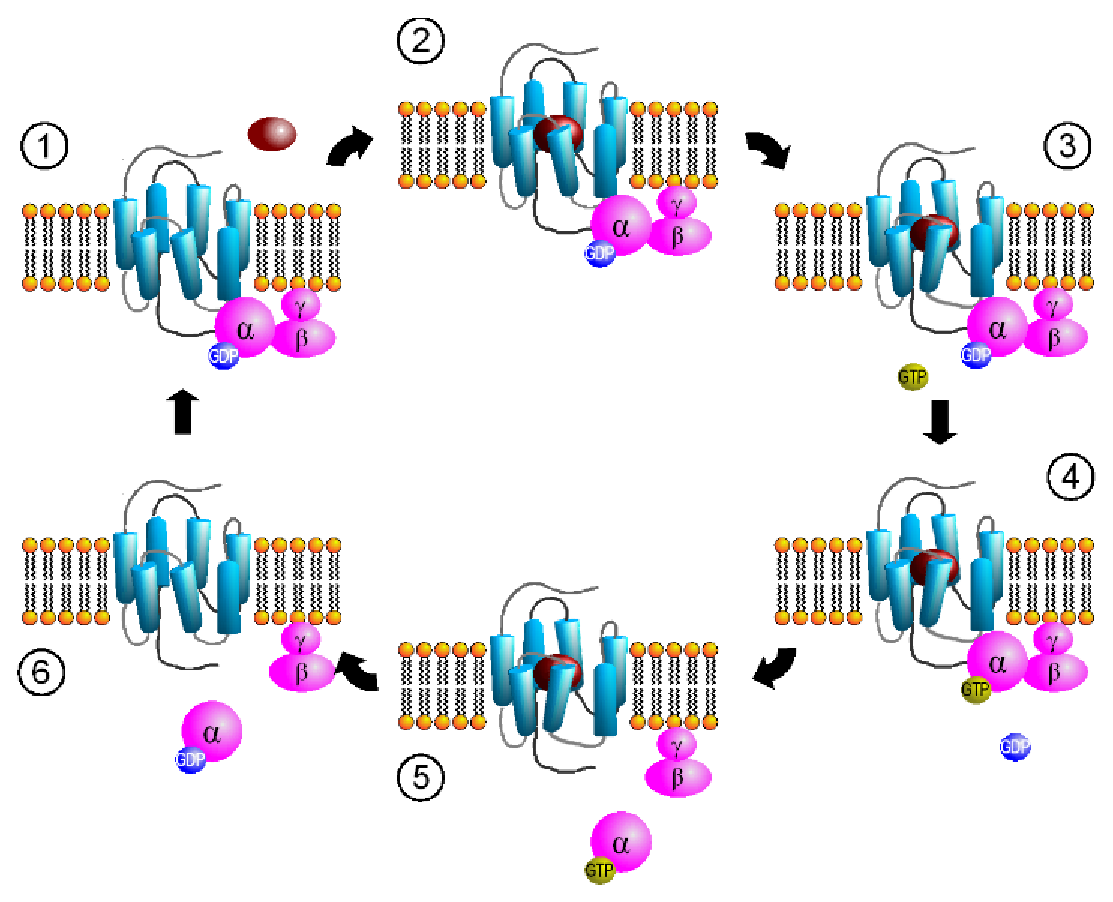
\includegraphics[height=7cm]{./images/G_protein_cycle.eps}}
\caption{G protein cycle}
\label{fig:G_protein}
\end{figure}

\subsection{small G proteins (monomeric small GTPase): Ras superfamily}
\label{sec:small-G-proteins}
\label{sec:Ras}
\label{sec:Rho}
\label{sec:Raf}
\label{sec:Rac}

Like their larger relatives (Sect.\ref{sec:G-protein}), small monomeric G
proteins (20-25 kDa) also bind to GTP and GDP to involve in signal
transduction. However, small GTPases are homologous to the alpha-subunit in
large G-protein complex.

small GTPases belong to the {\bf Ras superfamily of small GTPase}

G proteins that are members of the Ras, Rho, and Raf families, are referred to collectively as small
G proteins.

\textcolor{red}{\bf small GTPases}: 5 main families
\begin{enumerate}
  \item Rho
  \item Ras
  \item Ran
  \item Rab
  \item Arf
\end{enumerate}

\textcolor{red}{Ras}: is a superfamily of small GTPases and responsible for
cell proliferation; whic is divided into six subfamilies which share a common
core G domain (providing essential GTPase and nucleotide exchange activity)
\begin{enumerate}
  \item Ras
  \item Ral
  \item Rit
  \item Rap
  \item Rheb
  \item Rad
  \item Rit
\end{enumerate}

\textcolor{red}{Rho}: is a family of small G proteins (about 21 kDa); and is a
subfamily of Ras superfamily.

\textcolor{red}{Rac} (Ras-related C3 botulinum toxin): Rac are small
(about 21 kDa) signaling G proteins; they are subfamily of Rho-family of GTPases
\begin{enumerate}
  \item Rac1 (i.e. Ras substrate 1): activates PLC
  (Sect.\ref{sec:PLC-activators})
  
  there are different alternatively spliced version of Rac1 protein which
  appears to carry out different functions.
  
  \item Rac2:
  
  \item rac3
  
  \item RhoG: 
\end{enumerate}

\subsection{subtypes of 'large' G proteins}
\label{sec:G-protein_subtypes}

A (large) G-protein is protein complex, typicall a trimeric with 3 subunits
(alpha, beta, gamma), locating on the inside of the cell membrane and bind to
the membrane receptor called GPCR. By combination of different $\alpha$,
$\beta$, and $\gamma$ subunits, a great variety (>1000) G proteins can be produced.
Typically we write $G_\alpha$ and $G_{\beta\gamma}$ as the bega-gamma are
tightly associated subunits.

The G-protein complex is activated by a G protein-coupled receptor
(Sect.\ref{sec:GPCR}) and there are different types of GPCR.
\begin{itemize}
  \item $G_\alpha$ subunit: at rest, it binds to (1) a GDP molecule, (2) a
  tightly associated $G_{\beta,\gamma}$, and (3) a GPCR
  
  \item $G_{\beta,\gamma}$ subunits: The two subunits $G_\beta, G_\gamma$ are
  tightly associated, i.e. they can form a stable dimeric complex referred to as
  the beta-gamma complex. 

\end{itemize}
These subunits are in turn divided into several subclasses
(Sect.\ref{sec:G-protein_subtypes}) that acts as molecular switches
(Sect.\ref{sec:molecular-switch}) inside the cells, between inactivated form and
activated form (Sect.\ref{sec:G-proteins_activation-inactivation}).

Each member (at normal state) associates with a  receptor called G
protein-coupled receptor (Sect.\ref{sec:G-protein-coupled-receptor}).
G proteins in active form enable the signal from outside can be transmitted into
the inside of the cell via a proper signaling cascade of signal transduction
pathway (Sect.\ref{sec:G_protein_mediated-signaling-pathways}).


\subsection{\texorpdfstring{G-$\alpha$ subunits}{G-alpha subunits}}
\label{sec:G_alpha-subunits}

In ``large'' G protein, more than 15 identified G$\alpha$ subunits are divided
into 4 different subtypes of $G_\alpha$ subunit ($G_{\alpha s}, G_{\alpha i/o},
G_{\alpha q/11}, G_{\alpha 12/13}$).
A complete list of names of different G proteins is given in
\citep{Wettschureck2005}.
Some are listed in Table. \ref{tab:GPCR_ligand_Gprotein}, with its effectors are
given in Fig.\ref{fig:G_protein-function}.
	
% As $G_\alpha$ subunit is the one that performs signal transduction, there are
% different classes, Table \ref{tab:GPCR_ligand_Gprotein}:
\begin{enumerate}
  \item $G_s\alpha$ (s = stimulatory): - Sect.\ref{sec:Gs-protein}
  
  \item $G_i\alpha$ (i = inhibitory): - Sect.\ref{sec:Gi/o-protein}
  
  \item $G_o\alpha$ (o = other): - Sect.\ref{sec:Gi/o-protein} 
  
  \item $G_{q/11}\alpha$: - Sect.\ref{sec:Gq/11-protein}
  
  \item $G_{12/13}\alpha$: - Sect.\ref{sec:G12/13-protein}
\end{enumerate}


\begin{figure}[hbt]
 \centerline{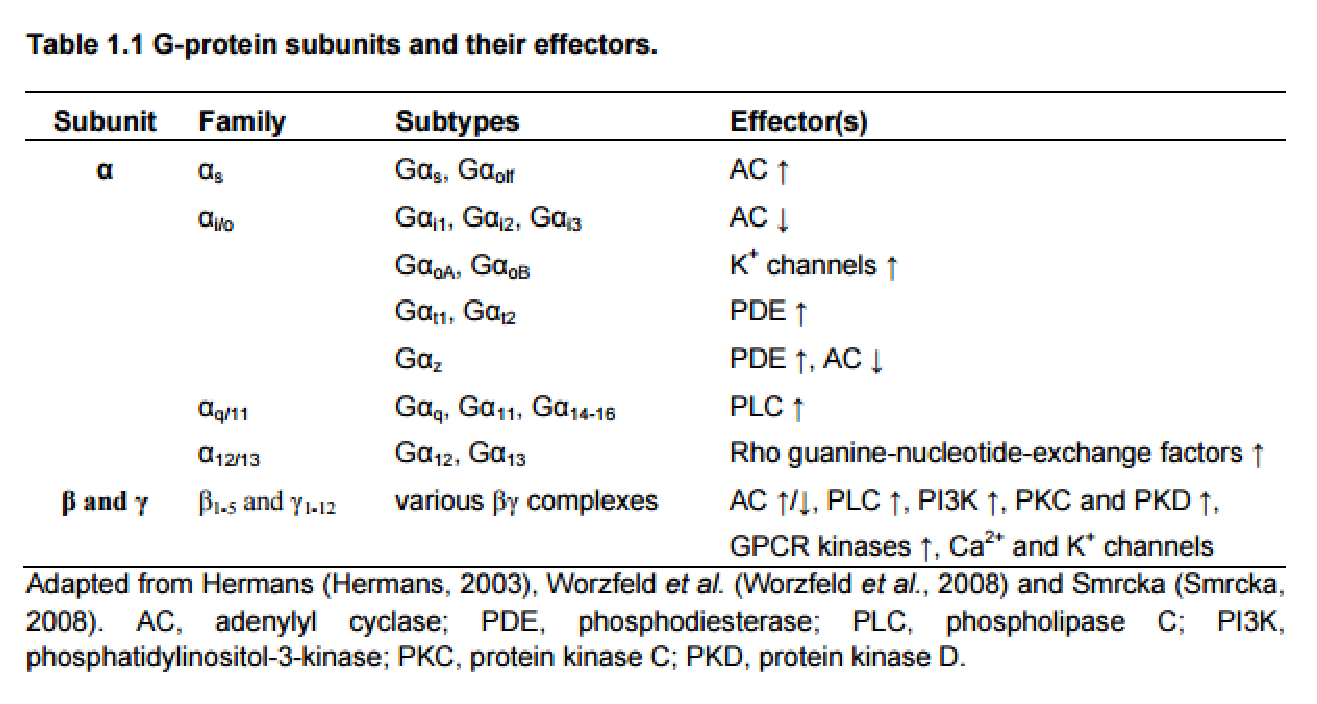
\includegraphics[height=7cm]{./images/Gprotein-summary.eps}}
\caption{The effector of different G proteins}
\label{fig:G_protein-function}
\end{figure}

% \begin{itemize}
%   \item more than 15 identified G$\alpha$ subunits are divided into 4 main
%   classes: G$\alpha$i/o, G$\alpha$s, G$\alpha$q, G$\alpha$12.
% \end{itemize}


\begin{table}[hbt]
\begin{center}
\caption{Ligands, GPCR receptor and coupling G proteins alpha subunit
(complete list: \citep{Wettschureck2005})}
\begin{tabular}{ccc} 
Ligand & GPCR & G-protein \\
  \hline\hline
epinephrine, norepinephrine  & $\beta_1$, $\beta_2$, $\beta_3$ & $G_s$ \\
dopamine & D1, D5 & \\
serotonin & 5-HT$_4$, 5-HT$_6$, 5-HT$_7$, 5-HT$_{5A/B}$ & \\

lisophosphatidid aid (LPA) & LPA$_{1/2/3}$ & $G_i$ \\
prostagladin D2 (PGD2) & CRTH2 & \\
 
glutamate & mGluR2,3,4,6,7,8 & $G_{i/o}$ \\
dopamine & D2, D3, D4 & \\
GABA & GABA$_{B1}$ (binding), GABA$_{B2}$ (signalling) & \\
succinate & GPR91 & \\
acetylcholine & M2, M4 &  \\
epinephrine, norepinephrine & $\alpha_{2A}$, $\alpha_{2B}$, $\alpha_{2C}$ & \\
histamine & H3, H4 & \\
melatonin & MT1, MT2, MT3 & \\
serotonin & 5-HT$_{1A/B/D/E/F}$ & \\ 

glutamate & mGluR1,5 & $G_{q/11}$ \\

pheromones & & $G_o$	\\
\hline
\end{tabular}
\end{center}
\label{tab:GPCR_ligand_Gprotein}
\end{table}


%\subsection{Go}


\subsection{Gi/o (and Gt, Gg)}
\label{sec:Gi/o-protein}
\label{sec:Go-protein}
\label{sec:Gi-protein}

{\bf Gi/Go family} ($G_{i/o}$) are widely expressed, with the members $\alpha$
subunit
\begin{itemize}
  \item Gi subunit
\begin{enumerate}
  \item $G_{i1}$
  
  \item $G_{i2}$
  
  \item $G_{i3}$ 
\end{enumerate}
All three types mediate the inhibition of various types of
adenylyl cyclase (Sect.\ref{sec:AC_adenylyl_cyclase}), i.e. decrease the
production of cAMP from ATP (Sect.\ref{sec:cAMP-dependent_pathway}). 

Gi/o subunit (or Gi subunit), once activated, inhibits the production of cAMP
from ATP.

  \item Go subunit
\begin{enumerate}
  \item G$\alpha_o$A: increase $\K$ channel activity
  
  \item G$\alpha_o$B: increase $\K$ channel activity
  
  \item G$\alpha_{t1}$: increase PDE production
  
  \item G$\alpha_{t2}$: increase PDE production
  
  \item G$\alpha_z$: increase PDE and inhibit AC production (which means
  inhibit the production of cAMP)

  $G_z\alpha$ is a less widely expressed member of $G_{i/o}\alpha$ family.
\url{http://en.wikipedia.org/wiki/Gi_alpha_subunit}

\end{enumerate}

{\bf Go family} is abundant in the nervous system, and is believed to perform
its function via $\beta\gamma$-complex
(Sect.\ref{sec:Gbetagamma-mediate-signaling-pathway}). Whether $G_o\alpha$ can
regulate effectors or not is not clear.

\end{itemize}

Also, their receptor-dependent activation results in the release of relatively
high amounts of $\beta\gamma$-complexes.
Thus, the activation of Gi/Go is belived the main mechanism for the activation
of $\beta\gamma$-mediated signalling processes
(Sect.\ref{sec:Gbetagamma-mediate-signaling-pathway}).


\begin{mdframed}

\textcolor{red}{\bf Gt, Gg}: Gt and Gg proteins are summarized under this label
due to sequence homologies.
Gt proteins, a.k.a. transducin, is used in the light recognition pathway in
retina cells. Gg protein occurs in the taste recognition for bitter.

\end{mdframed}

Gi/o is activated upon the activation of these receptors  
\begin{enumerate}
  \item M2-receptor (Sect.\ref{sec:M2-receptor}) and M4-receptor
  (Sect.\ref{sec:M4-receptor})
  
  \item Alpha-2 ($\alpha_2$) adrenergic receptor (Sect.\ref{sec:alpha-adrenergic-receptor}) 
\end{enumerate}
\url{https://en.wikipedia.org/wiki/Gi_alpha_subunit}

Recent data provide evidence that heterotrimeric G proteins of the Gi family are
also involved in receptor-independent processes (check
Sect.\ref{sec:Ras-GTPase}).




\subsection{Gs}
\label{sec:Gs-protein}
\label{sec:Golf-protein}

Gs subunit is ubiquitously expressed with 2 types
\begin{itemize}
  \item G$\alpha$s member
  
  \item G$\alpha$olf member: These G proteins are used in the signal transduction of taste and smell.
  
\end{itemize}

Both types activates adenylyl cyclase (AC) resulting in increase of [cAMP] by
stimulating the production of cAMP from ATP (Sect.\ref{sec:cAMP-dependent_pathway}).

%The Gs family has
% {\bf Gs family} is ubiquitously expressed, which activates adenylyl cyclase
% (AC) resulting in increase of [cAMP] (Sect.\ref{sec:cAMP-dependent_pathway}).

Gs proteins link to the following GPCRs
\begin{enumerate}
  \item Beta ($\beta_1$, $\beta_2$ and $\beta_3$) adrenergic receptor
  (Sect.\ref{sec:beta-adrenergic-receptor}) activated by catecholamine
  (Sect.\ref{sec:Catecholamines}) in cardiac myocyte.
  
  \item H2 receptor (Sect.\ref{sec:histamine-receptors})
\end{enumerate}

\subsection{Gq/11}
\label{sec:Gq/11-protein}

{\bf Gq/G11 family} ($G_{q/11}$) includes 
\begin{itemize}
  \item G$\alpha$q
  
  \item G$\alpha$11
  
  \item G$\alpha$14-16

The $\alpha$-subunis of this family are ubiquitously expressed (e.g. G12, G13),
except $G_{\alpha14}$ and $G_{\alpha15/16}$ 
[NOTE: $G_{15}\alpha$ is in murine, while
$G_{16}\alpha$ is in human].

\end{itemize}

Gq/11 proteins are preassembled (pre-coupled) with the following GPCRs,
and the common polybasic domain in the C-tail of Gq-coupled receptors is
necessary for the receptor-G protein preassembly \citep{qin2011}
\begin{enumerate}
  \item 5-HT$_2$ receptor (Sect.\ref{sec:5-HT_receptor})
  
  \item Muscarinic receptors: M1, M3 and M5 (Sect.\ref{sec:muscarinic-acetylcholine-receptor})
  
  \item mGluR group I: Sect.\ref{sec:mGluR_group-1}
  
  \item Alpha-1 ($\alpha_1$) adrenergic receptor (Sect.\ref{sec:adrenergic_receptor})
  
  \item H1 receptor (Sect.\ref{sec:histamine-receptors})
\end{enumerate}

Upon the activation of the above receptors with a selective agonist, these
proteins are release and then bind to activate PLC$\beta$
(Sect.\ref{sec:PLC-beta}), which then leads to subsequent production of
inositol-1,4,5-trisphosphate (IP3), diacylglycerol (DAG), and protein kinase C
(PKC) stimulation. NOTE: They are good activators of $\beta1-$, $\beta3-$ and
$\beta4-$ isoforms of phophoslipase C (PLC), but not of $\beta2$-PLC.


Active PKC (Sect.\ref{sec:PKC}) and Ca2+ signals could then engage in the
modulation of diverse metabotropic activities.




\subsection{G12/13}
\label{sec:G12/13-protein}

G12/13 is activated upon the activation of these receptors
\begin{enumerate}
  \item thromboxan receptors and 
  
  \item thrombin receptors
\end{enumerate}

Their effector proteins are unknown.

%We will not focus on this as it is not found in synapse.

The G12/13 family is probably the least well characterized subtype, partly
because G12/13 coupling is difficult to determine when compared with the other
subtypes.

The G12/13 family have been shown to induce Rho activation and Rho-dependent
biological responses, including stress fiber formation and focal adhesion
assembly.

The G12/13 family are best known for their involvement in the processes of cell
proliferation and morphology, such as stress fiber and focal adhesion formation.
Interactions with Rho guanine nucleotide exchange factors (RhoGEFs) are thought
to mediate many of these processes. (Buhl et al.1995, Sugimoto et al. 2003).
Activation of Rho or the regulation of events through Rho is often taken as
evidence of G12/13 signaling. Receptors that are coupled with G12/13 invariably
couple with one or more other G protein subtypes, usually Gq.

\url{http://www.pathwaycommons.org/pc/record2.do?id=485716}

\url{https://en.wikipedia.org/wiki/Rho_family_of_GTPases}

\subsection{activation/inactivation mechanism}
\label{sec:G-proteins_activation-inactivation}

% \begin{mdframed}
% % hydrolyze GTP (which took
% % place in the G domain - Sect.\ref{sec:G-protein}) 
% GTPase:
% \begin{itemize}
%   \item active form: GTP-bound
%   
%   \item inactive form: GDP-bound
%   
%   \item 
% \end{itemize}
% \end{mdframed}

GTPase (G protein) in
\begin{itemize}
  \item {\bf inactivated G protein} (GDP-bound):
  G$_\alpha$-GDP-G$_{\beta\gamma}$

An in-activated G protein has a GDP-bound at $\alpha$-subunit.
In inactivated state, the G protein can be free from GPCR, or be bound by GPCR,
depending on the types of G proteins (Sect.\ref{sec:G_alpha-subunits}).
In either way, G proteins, located inside the cells, are activated by GPCR
(Sect.\ref{sec:G-protein-coupled-receptor}).

\textcolor{red}{\bf inactive $\rightarrow$ active form}:
\begin{itemize}
  \item Traditional view (G protein already associated with GPCR):
  confirmed with Gq/11 (Sect.\ref{sec:Gq/11-protein})
  
Upon ligand binding (Sect.\ref{sec:GPCR_ligands}) at the GPCR at the
extracellular side, it changes the intracellular domain of GPCR, which enables
GPCR to function as a GEF (guanine nucleotide exchange factor) that causes the
GDP to dissociate, and GTP which is abundant in the cytosol then bind to G
protein, Fig.\ref{fig:G_protein}.

Compared to GDP, GTP has an additional phosphate group.
This extra phosphate holds the two switch regions in a "loaded-spring"
configuration (specifically the Thr-35 and Gly-60).
In terms of concentration, there is little evidence that GTP is about 10-fold
to 30-fold higher than GDP which was made in frog oocytes; while many results
suggested closely equal concentrations and in the range 1-2.5 mM (review:
\citep{nelson2008_GTP-GDP}).
 

  \item Modern view (G protein free from GPCR):
  
Upon ligand binding (Sect.\ref{sec:GPCR_ligands}) at the GPCR at the
extracellular side, it changes the intracellular domain of GPCR, 
making GPCR becomes highly affine for G protein-GDP complex. 
On binding with the complex, the next stages is just like above, i.e.
GPCR function as a {\bf GEF (guanine nucleotide exchange factor)} that causes
the GDP to dissociate, and GTP which is abundant in the cytosol then bind to G
protein, Fig.\ref{fig:G_protein}.
  
\end{itemize}  


  \item {\bf activated G protein} (GTP-bound):

% ``large'' intracellular G protein is activated by a conformation change in GPCR
% (due to proper ligand binding) - Sect.\ref{sec:GPCR_ligands}) which leads to the
% dissociation of a G protein subunit from the receptor. At the same time, that
% process trigger the binding from GDP to GTP, as shown in Fig.\ref{fig:G_protein}.
% Once there is a proper ligand binding to GPCR, it triggers the change its
% intracellular conformation, which leads to the dissociation of G protein.

At the activated form (G protein-GTP complex), upon GTP binding, it causes a
conformational change in G protein, activating both the $\beta$ and $\gamma$
subunits. Depending on the situations
\begin{itemize}
  \item $\beta$ and $\gamma$ subunits separate from the G$_\alpha$-GTP.
  
NOTE: This is the {\it traditional view}.  
$G_\alpha$-GTP is dissolved from the tightly associated
$G_{\beta\gamma}$ subunits and go to activate other proteins during its
transduction pathway.
  
  \item $\beta$ and $\gamma$ subunits keep binding to $\alpha$ subunit.

NOTE: models which suggest molecular rearrangement, reorganization, and
pre-complexing of effector molecules are beginning to be accepted.
Inded, the interaction of G proteins with the inner side of the plasma membrane
is facilitated by lipid modifications of both the $\alpha$-subunit as well as of
the $\beta$-subunit of the $\beta\gamma$-complex \cite{Wettschureck2005}.

The dissociated activated G-protein ultimately going on to regulate downstream
cell processes. 

\end{itemize}
So, in either cases,  both $G_\alpha$-GTP and G$\beta\gamma$ can then activate
different and/or the same signaling cascades, which send the signal
further down the signal reaction chains and finally results in a change in cell
function (Sect.\ref{sec:G_protein_mediated-signaling-pathways}).

\end{itemize}

\textcolor{red}{\bf  active $\rightarrow$ inactive form}: GTP is hyrolyzed into
GDP through intrinsic GTPase-activity. This process is accelerated by {\bf RGS protein}
(Sect.\ref{sec:RGS_protein}) - which acts as {\bf GTPase-activating proteins
(GAPs)} and are specific for G$\alpha$ subunits.
\begin{itemize}
  \item It can be reversed (switching the GTPase on again) by {\bf Guanine
  nucleotide exchange factors} (GEFs), which cause the GDP to dissociate from the GTPase, leading to
G protein association with a new GTP.
\end{itemize}
If no reverse, $G_\alpha$-GDP reassociate with G$\beta\gamma$.  This bring G
protein backs to inactivated state.
\url{https://www.youtube.com/watch?v=V_0EcUr_txk}

\textcolor{red}{\bf long stimulation}: If the ligand keeps binding to the GPCR,
the G proteins will be reactivated.
Upon this long simulation, however, GPCR eventually become inactivated, even if
the ligand is still binding. To do so, a {\bf G-protein coupled receptor kinases
(GKR)} is involved to regulate GPCR. GKR phosphorylate the cytosolic portion of
the activated GPCR. Once the cytosolic portion is phosphorylated, it binds to
{\bf arrestin}, which inactivate the GPCR and precludes the G protein activation
\citep{Ribas2007}.
\url{http://en.wikipedia.org/wiki/G_protein-coupled_receptor_kinase}

\textcolor{red}{\bf efficiency of signal transduction}:
The efficiency of the signal transduction via a GTPase depends on the ratio of
active to inactive GTPase
\begin{equation}
\frac{\text{GTPase-GTP}}{\text{GTPase-GDP}} =
\frac{k_\text{diss.GDP}}{k_\text{cat.GTP}}
\end{equation}
with $k_\text{diss.GDP}$ (the dissociation constant of GDP), and
$k_\text{cat.GTP}$ (the hydrolysis constant of GTP for a specific GTPase).
It is regulated by
\begin{itemize}
  \item (making more efficient): GEF speed up the dissociation of GDP, and thus
  accelerate the increase [active GTPase]
  
  \item (making less efficient): Guanine nucleotide dissociation inhibitors
  (GDIs) inhibits the dissociation of GDP, and thus slow down the increase
  of [active GTPase]
  
  \item (making less efficient): GAP speed up GTP hydrolysis, and thus making
  less [active GTPase] available by the conversion from [active GTPase] to
  [inactive GTPase]
  
\end{itemize}

\url{https://www.youtube.com/watch?v=NB7YfAvez3o}

\subsection{RGS protein}
\label{sec:RGS_protein}

RGS protein is Regulator of G protein signalling and is specific to G$\alpha$
subunit. RGS protein is also able to increase the GTPase activity on
$G_\alpha$-subunits, bringing G protein backs to inactivated state quickier.

There are about 30 RGS proteins found, which have selectivities on
$G_\alpha$-subfamilies.


\subsection{Ras GTPase}
\label{sec:Ras-GTPase}

Ras GTPase (small GTPase) or Ras is a G protein relates to the G$_\alpha$
subunit in 'large' G protein with 21 kDa.
Ras is attached to the cell membrane.

Ras superfamily is further divided into five subfamilies: Ras, Rho, Rab, Arf and
Ran. The Rho subfamily is further divided into RHOA, RAC1, and CDC42.	

The 3 Ras genes in humans (H-ras, K-ras, and N-ras) are the most common
oncogenes in human cancer; mutations that permanently activate Ras are found in
20\% to 25\% of all human tumors and up to 90\% in certain types of cancer
(e.g., pancreatic cancer).

Ras contains a six-stranded beta sheet and 5 alpha helices
\begin{itemize}
  \item G domain (166 amino acids) with 5 G motifs and bind GDP/GTP directly.
  The change in G2 and G3 motifs, upon GTP binding, is what mediates the basic
  functionality as a molecular switch protein.
  
  NOTE:  GTP bound state of Ras is On-state and GDP bound state is the
  Off-state.
  
  
  \item C terminal membrane targeting region  
\end{itemize}

\textcolor{red}{\bf Activation mechanism}: 
\begin{itemize}
  \item like many other G protein, the activation is similar to what described
  in Sect.\ref{sec:G-proteins_activation-inactivation}
  
  \item Ras has an intrinsic GTPase activity, which means that the protein on
  its own will hydrolyze a bound GTP molecule into GDP.
  
  However this process is too slow for efficient function, and hence the GAP for
  Ras, RasGAP, may bind to and stabilize the catalytic machinery of Ras,
  supplying additional catalytic residues ("arginine finger") such that a water
  molecule is optimally positioned for nucleophilic attack on the
  gamma-phosphate of GTP.
   
\end{itemize}

{\bf Affectors}: those that allow GTP-Ras to carry out its functions
\begin{itemize}
  \item PI3K
\end{itemize}

Ras activates several pathway
\begin{itemize}
  \item  mitogen-activated protein (MAP) kinase cascade
  
  \item AKT cascade: 
  
  \item Ras also binds a magnesium ion which helps to coordinate nucleotide binding.
  
  %Upon GDP dissociation by GEF, 
\end{itemize}

\section{GPCR ligands}
\label{sec:GPCR_ligands}

GPCR ligands refers to different ligands that can bind and activate GPCR
\begin{itemize}
  \item odors
  \item pheromones
  \item hormones 
  \item neurotransmitters 
  %- Sect.\ref{sec:neurotransmitter} $\rightarrow$ the
  %GPCR of this type is called adrenergic receptor
  %(Sect.\ref{sec:adrenergic_receptor})
  \item paracrine factors
  \item cannabinoid - Sect.\ref{sec:cannabinoid-receptors}
\end{itemize} 

Most of GPCR code for sensory receptors, e.g. taste or olfactory receptors using
odors or pheromones. About 400-500 GPCRs code for non-sensory ligands like
hormones, neurotransmitters, or paracrine factors. The discussion about
neurostransmitters is in Sect.\ref{sec:neurotransmitter}.

A complete list of
\begin{verbatim}
ligands  -- GPCR receptor -- coupling G protein
\end{verbatim}
can be referenced in \citep{Wettschureck2005}.
Here we list some of them in Table.\ref{tab:GPCR_ligand_Gprotein}.


\section{GPCR in neurons}
\label{sec:GPCR-in-neurons}

Sect.\ref{sec:G-protein-coupled-receptor} discusses how we classify G
protein-coupled receptors. In this section, we will learn what types of GPCR are
available on the pre-synaptic side and post-synpatic side of different types of
neurons. \textcolor{red}{In the brain, different areas have different Dopamine receptor
subtypes densities} (Sect.\ref{sec:dopamine_receptors}).


\citep{Wettschureck2005}

\subsection{presynaptic activation}

NOTE: Presynapse is on the axonal-side (Sect.\ref{sec:synapse}), at which
neurotransmitters are release.

Inhibitory effects of neurotransmitter release is mediated by GPCR
(Sect.\ref{sec:G-protein-coupled-receptor}) likes
\begin{itemize}
  \item $\alpha2$-adrenoreceptor
  \item $\mu-$ and $\delta-$ opioid receptors
  \item GABA$_B$ receptor
  \item adenosine A$_1$
  \item endocannabinoid CB$_1$-receptor
\end{itemize}
They all couple to G proteins of Gi/Go family (Sect.\ref{sec:G-protein_subtypes}).
The inhibitory is done via inhibitory modulation of action potential (AP)-evoked
$\Ca$ entry to the presynaptic terminal \citep{augustine1985}. This $\Ca$ entry
is required to trigger neuotransmitter release, so by blocking this entry, it
inhibits the signal pathway. 

In nerve cells, N-type and P/Q-type $\Ca$ channels are concentrated at
terminals (Sect.\ref{sec:N-and-P/Q-type}). Along with R-type $\Ca$ channels
(Sect.\ref{sec:R-type_Ca-channel}), these $\Ca$ channels are inhibited due to
the interaction of the $\beta\gamma$-complex of the activated G protein with the
$\alpha$-subunit of the $\Ca$ channels Ca$_v$2.1-2.3, which block the channel
pore.

At the presynaptic terminal, there are also GIRK (G protein-coupled inwardly
rectifying $\K$) channels. GIRK channels are
well-established effectors of G$\beta\gamma$-complex, which activates GIRK.
However, their physiological role is unclear.

Recent evidence suggested a potential role of {\bf syntaxin 1} - a presynaptic
ion channel - as a key element in the inhibition of N-type $\Ca$ channels by
G$\beta\gamma$-complex.

\subsection{synaptic (postsynaptic) transmission}
\label{sec:synaptic_transmission}
\label{sec:postsynaptic_transmission}

NOTE: Postsynapse refers to the dendritic-side of a synapse
(Sect.\ref{sec:synapse}), at which the received signals is transmitted along the
dendrite to the soma, then to the axon.

The modulation of synaptic transmission has best been described at the parallel
fiber (PF)-Purkinje cell (PC) synapse in the cerebellum (see synaptic potential
- Sect.\ref{sec:synaptic_potential}).

The activation of two G$\alpha$ subunits (Gq and G11) mediate the effects of
metabotropic glutamate group 1 receptors (Sect.\ref{sec:mGluR_group-1}). The
pathway is called Gq/G11-mediated IP3-dependent transient increase in dendritic
[$\Ca$], which does not requires the change in membrane potential $V_m$. This
pathways is important for long-term depression (LTD) at the PF-PC synapse.
LTD (Sect.\ref{sec:LTD}) is believed to be one of the cellular mechanisms
underlying cerebellar motor learning \citep{fino2010}.



\section{GPCR in cardiac cells}

Sect.\ref{sec:G-protein-coupled-receptor} discusses how we classify G
protein-coupled receptors. In this section, we will learn what types of GPCR are
available on the plasmamembrane of the different types of cardiac cells, with
the focus on ventricular myocytes.

\citep{Wettschureck2005}

\section{Proprioceptor}
\label{sec:proprioceptor}

In the limbs, the {\bf proprioceptors} are sensors that provide information
about joint angle, muscle length, and muscle tension, which is integrated to
give information about the position of the limb in space.
They locate in muscles, tendons, joints, and the inner ear, that detects the
motion or position of the body or a limb.

The {\it muscle spindle} is one type of proprioceptor that provides information
about changes in muscle length.

\section{Vestibular receptor}
\label{sec:vestibular_receptor}

The vestibular system deals with the body's sense of balance (head and eye
movement). It has 5 distinct end organs: 3 semicircular canals that are
sensitive to angular accelerations (head rotations) and 2 otolith organs that are sensitive
to linear (or straight-line) accelerations.
\url{http://emedicine.medscape.com/article/883956-overview}

Within the vestibular organs there are vestibular receptors , which are hair
cell mechanoreceptors.

\section{*2. Glutamate receptors}
\label{sec:glutamate_receptor}

Glutamate receptors refer to a family of transmembrane protein that is activated
upon the binding of  the neurotransmitter called amino acid glutamate 
(Sect.\ref{sec:Glutamate}).

Glutamate released from the presynaptic side (i.e. synaptic terminal) binds to
and activates glutamate receptors primarily on postsynaptic side membranes of
neuronal cells. However, the recent discovery of presynaptic glutamate receptors
in some neurons have added the complexity to the way we view glutamatergic
synaptic transmission (review: \citep{pinheiro2008}).


There are two classes of glutamate receptors, and they are responsible for the
{\it glutamate-mediated postsynaptic excitation} of neural cells, and are
important for neural communication, memory formation, learning, and regulation.

\begin{enumerate}
  
  \item (excitatory) {\bf ionotropic glutamate receptors} (iGluR -
  Sect.\ref{sec:iGluR}): the ion-permeable channels. The permeated ions performs
  the intracellular function.
  
  There are three types: NMDA receptors (Sect.\ref{sec:NMDAR}), AMPA receptors
  (Sect.\ref{sec:AMPAR}), and kainate receptor
  (Sect.\ref{sec:kainate_receptor}).
  
  \item (can be excitatory or inhibitory of postsynaptic cells) {\bf
  metabotropic glutamate receptors} (mGluR, Sect.\ref{sec:mGluR}):
  triggering the G protein signaling, i.e. a G-protein signalling cascade
  (Sect.\ref{sec:G_protein_mediated-signaling-pathways}).
  
  mGluR are G-protein coupled receptor, and they belong to group C family of
  GPCR (Sect.\ref{sec:G-protein-coupled-receptor}).
  
\end{enumerate}

According to the most simplistic view, the two families of glutamate receptors
have distinct role in neuronal activity:
\begin{itemize}
  \item postsynaptic iGluR: direct and fast information transfer
  
  
  \item postsynaptic mGluR: 

Unlike the excitatory iGluR, mGluRs cause slower
postsynaptic responses that can either increase or decrease the excitability of
postsynaptic cells. Hence the physiological roles of mGluRs are quite varied.


  \item presynaptic iGluR + presynaptic mGluR: control the strength of synaptic
  transmission by altering the likelihood of synaptic vesicles release in
  response to an incoming AP
  
  \begin{itemize}
    \item presynaptic iGluR:  Sect.\ref{sec:iGluR-presynaptic}
    
    \item presynaptic mGluR:  Sect.\ref{sec:mGluR-presynaptic}
  \end{itemize}
\end{itemize}


\section{-- iGluR: inotropic glutamate receptors}
\label{sec:inotropic-glutamate-receptors}
\label{sec:iGluR}

Ionotropic glutamate receptors (iGluRs) 
$^\text{[{\it inotropic = affect the force of muscle contraction}]}$ includes
the NMDA-receptors - Sect.\ref{sec:NMDAR}, and non-NMDA-receptors
(Sect.\ref{sec:non-NMDA-receptor}.

%There is a third subclass called {\bf kainate receptors}

%\subsection{NMDA}
\label{sec:NMDA}
%\subsection{APMA}
\label{sec:AMPA}
\begin{mdframed}

NMDA stands for {\bf N-methyl-D-aspartic acid}. 
NMDA is a water-soluble synthetic substance that is not normally found in
biological tissue. NMDA can acts as a ligand exclusively on a subtype of
glutamate receptors (Sect.\ref{sec:glutamate_receptor}) 

% The binding of glutamate to NMDAR will activate this Ca-channel

AMPA stands for $\alpha$-amino-3-hydroxy-5-methyl-4-isoxazolepropionic
acid is another synthetic substance that can act exclusively on a subtype of
glutamate receptor.
\end{mdframed}

% as glutamate, an agonist at NMDA receptor (NMDAR -
% - the predominant
% molecular device for controlling synaptic plasticity (a mechanism for memory and learning). 

\section{---- non-NMDA receptors (AMPA/Kainate receptor)}
\label{sec:AMPA/Kainate-receptor}
\label{sec:non-NMDA-receptor}

Non-NMDA-receptors is a type of inotropic GluR (iGluR - Sect.\ref{sec:iGluR}).
Its other name is {\bf AMPA/kainate receptors}, which were originally classified
by their activation of agonist quisqualate and kainate, but not NMDA.
The use of quisqualate has now been abandoned in favour of the more selective
agonist AMPA.

% divided into AMPA receptors
% (AMPARs - Sect.\ref{sec:AMPAR}) and kainate receptors (KAR) (Sect.\ref{sec:kainate_receptor}). 

The classification into AMPAR or Kainate receptors depends upon the subunits
forming the channel which is a tetramer
\begin{itemize}
  \item GluR1 - GluR4: four glutamate receptor subunits that can be regarded as
  AMPA receptor (AMPAR) - Sect.\ref{sec:AMPAR}
  
  \item GluR5 - GluR7, and KA1, KA2: five glutamate receptor subunits that can
  be regarded as Kainate receptor (KAR) - Sect.\ref{sec:kainate_receptor}

GluR5 - GluR7 are thought to correspond to the low-affinity Kainate receptor;
whereas KA1 and KA2 correspond to the so-called high-affinity Kainate receptors.

\end{itemize}
Even though the subunits can form homogeneous or heterogeneous channel
assemblies with other members in the same or different group.
Immunoprecipitation experiments showedthat GluR6 and/or GluR7 subunit can
assemble with KA2; but not with GluR2-GluR4.

Desensitization is a widely accepted property of non-NMDAR
(Sect.\ref{sec:desensitizing-response}), where channels open, then become closed
even with ligand-binding. 

\subsection{-- agonist/antagonist}

Even though both AMPA and Kainate can activate non-NMDAR, each may have a
different affinity to the receptor. Kinate can activate AMPAR; and AMPAR can
activate most of the Kainate receptors.

All AMPAR and Kainate receptors appear to be blocked by the competitive
antagonist CNQX and NBQx; although these antagonists appear to show selectivity
to native AMPAR.

Some novel non-competitive antagonists (e.g. GYKI52466) also appear to have
selectivity to AMPAR compared to Kainate receptors.

The dye Evans Blue have been show to block receptors formed by all combinations
of GluR1-GluR4 apart from GluR3 and GluR6.

The novel compound NS-102 can antagonize GluR6, but not GluR2/4.

LY328884 can antagonise kainate receptors that contain GluR5.

GYKI 53655 is the AMPAR-antagonist that unmask AMPAR from KAR.


\subsection{AMPAR}
\label{sec:AMPAR}

AMPA receptors is one type of non-NMDA iGluR (Sect.\ref{sec:non-NMDA-receptor}).
that is activated upon binding of glutamate neurotransmitter
(Sect.\ref{sec:Glutamate}) and also the strong agonist is
AMPA (Sect.\ref{sec:AMPA}, i.e. AMPA can mimics the effect of glutamate. Models
of AMPAR are discussed in Chap.\ref{chap:AMPAR-models}.

\subsection{-- isoforms}
\label{sec:AMPAR-isoforms}

AMPA receptor is a tetramer formed by four types of subunits:
GluR1-4 subunits (aka GluRA - GluRD) which differ most in their C-terminal
sequence. Most AMPARs are heterotetrameric, consisting of symmetric 'dimer of
dimers' of GluR2 and either GluR1, GluR3 or GluR4. \textcolor{red}{Example}: in
mature hippocampus:   2$\cdot$GluR1 + 2$\cdot$GluR2 (aka GluR1/2), 2$\cdot$GluR2
+ 2$\cdot$GluR3  (aka GluR2/3).

NOTE:
\begin{itemize}
  \item GluR1 (GluRA or GluA1)
  \item GluR2 (GluR-B or GluR-A2)
  \item GluR3 (GluR-C or GluR-A3)
  \item GluR4 (GluRD or GluA4) = GluRA-D2
\end{itemize}

The subunits have the same extracellular N-terminal and TM domains; but
different C-terminal  cytoplasmic tail region, i.e. result in binding to
different proteins. A region on the C-terminal region of NMDA receptors called
the tSXV motif that has the ability to bind to the PDZ domain (Ehlers et al.,
1996)

\begin{itemize}
  \item GluR1, GluR4 (with long C-tail): binds to protein 4.1N and PDZ domain of
  SAP97 (Sect.\ref{sec:SAP97})
  
  Long C-tails prevent GluR1/4 receptors from being inserted directly into the
  postsynaptic density zone (PSDZ) in the absence of activity, whereas the short
  C-tails of GluR2/3 receptors allow them to be inserted directly into the PSDZ
  
  \item GluR2, GluR3 (shoter C-tail): binds to PDZ domain of GRIP/ABP and PICK1
  proteins. GRIP anchors GluR2-containing AMPAR to the postsynaptic density
  (PSD95 - Sect.\ref{sec:PSD}).

GluR2 C-terminal can quickly bind to protein interacting with C-kinase1
(PICK1), N-ethylmaleimide-sensitive fusion protein (NSF - an ATPase involved in
membrane fusion events), and GRIP1/ABP protein (Sect.\ref{sec:GRIP}). This
allows rapid insertion of GluR2-containing AMPA receptors at the synapse.
GluR2/3 subunits are more stably tethered to the synapse than GluR1 subunits.

The unique role of GluR2 is determined by the single amino acid residue in the
second hydrophobic region (M2); which is arginine (R); while in other subunit it
is glutamine (Q). This location is known as Q/R site.
When the arginine in this site is replaced with glutamine, the receptor shows
marked inward rectification and high $\Ca$ permeability.
Interestingly, this Q/R site is not encoded on the GluR2 genomic DNA but
introduced by RNA editing - whose process is developmentally regulated.
In embryos, a small percentage of the GluR2 is not edited, and therefore the
unedited form (GluR2Q) coexists with the edited form (GluR2R).
Postnatally, however, virtually all GluR2 exists in the edited form (Sommer et
al., 1991; Burnashev et al., 1992).

NOTE: Beside Q/R substitution at M2 in GluR2; there is also R/G substitution at
site betwen M3 and M4 in GluR2/3/4 subunit.

\end{itemize}
   
\begin{mdframed}
So, each AMPA receptor has 4 binding sites (formed by the extracellular
N-terminal and  extracellular loop between transmembrane domains three and
four), one for each subunit. When an agonist binds, these two loops move towards
each other, opening the pore. Having two bound sites is enough to open AMPAR.

The presence of a GluR2 subunit is determined by post-transcriptional
modification - RNA editing - of the Q-to-R editing site of the GluR2 mRNA.
\textcolor{red}{The prevention of calcium entry into the cell on activation of
GluR2-containing AMPARs is proposed to guard against excitotoxicity}

\end{mdframed}

\subsection{-- GluR2-containing AMPAR}
\label{sec:AMPAR-GluR2}
\label{sec:AMPAR-GluR2/3}

Postnatally, virtually all GluR2 exists in the edited form, i.e. GluR2(R)
(Sommer et al., 1991; Burnashev et al., 1992). GluR2(R) subunit plays a key role
in determining the functional properties of AMPAR, such as rectification
properties and $\Ca$ permeability.

Receptors with GluR2 exhibit either linear or outwardly rectifying
current-voltage (I-V) relationships and little $\Ca$ permeability.

\subsection{-- GluR2-lacking AMPAR}
\label{sec:AMPAR-GluR1}
\label{sec:AMPAR-GluR3}

GluR2-lacking AMPAR show strongly inward rectification and high $\Ca$
permeability (Koike, Ozawa, 2000).


\subsection{-- splicing variant:flip and flop}
\label{sec:AMPAR-flip-flop}

Apart from multiple subunit types, the molecular diversity of AMPAR subunits is
further increased by the presence of splicing variants. Alternative splicing in
the extracellular ligand binding domain of the AMPA receptors generates two
variants, i.e., flip and flop, generated by alternative splicing of a 115 bp
region immediately preceding M4 (Sommer et al., 1990; Monyer et al., 1991)

\begin{enumerate}
  \item flop variant of mGluR2-AMPAR is known to desensitize faster 
  than flip - Sect.\ref{sec:AMPAR-desensitization}
  
  \item at single channel level: flop variant of GluR2 opens the channel,
  following the binding of glutamate, with the same rate as the flip channel,
  but closes its channel more rapidly.
  

  
  \item 
\end{enumerate}


\subsection{-- permeability}
\label{sec:AMPAR-permeability}

The AMPAR's permeability to calcium and other cations, such as sodium and
potassium, is governed by the GluR2 subunit (Sect.\ref{sec:AMPAR-GluR2}). If an
AMPAR lacks a GluR2 subunit, then it will be permeable to sodium, potassium, and
calcium. The presence or absence of GluR2 subunit characterizes physiological
properties of AMPA receptors.


\begin{itemize}

  \item rat cerebellar Purkinje cell (Hausser, Roth, 1997): dendritic and
  somatic AMPARs contain GluR2-subunit with rapid kinetics and low 
  permeability to $\Ca$, i.e. $P_\ca/P_{\text{Cs}} = 0.053$.
  
  The single channel conductance is estimated 8 pS. in dendritic and somatic
  patches, with maximum $P_o$ at 0.7 at 5 mM Glut.

  \item  {\bf GluR2-containing AMPAR}: are $\Ca$ impermeable and have
  linear rectification pattern, whereas 

AMPA receptors are non-selective cationic channels allowing the passage of Na+
(in) and K+ (out) and therefore have an equilibrium potential near 0 mV.
The single channel conduction is 20 pS.

The undergoes RNA editing in GluR2 resulting in a switch of a glutamine residue
(Q607) in the pore-lining region of the subunit to an arginine (R607),
making GluR2-containing AMPAR impermeable to Ca2+ and resistant to blockade by
intracellular polyamines.
 
  \item {\bf GluR2-lacking AMPAR}: are $\Ca$ permeable (i.e. the channel
  permeate to both $\Na, \K$ and $\Ca$) and have inward rectification I-V curve
  pattern.

If an AMPAR lacks GluR2 subunits, then it is susceptible to being blocked in a
voltage-dependent manner by a class of molecules called polyamines.
  
\end{itemize}


\subsection{-- AMPAR's cellular distribution}
\label{sec:AMPAR-distribution}

While the cellular localization of AMPA-type subunits in the basal ganglia has
been well characterized in rodents, the cellular localization of AMPA subunits
in primate basal ganglia is not. 

\begin{mdframed}

NOTE: Immunohistochemical, {\it in situ} hybridization histochemical (ISHH), and
RT-PCS can be used to examined the localization of AMPAR subunits in striatal
neurons; but they does not provide relative frequency and abundance.

LM and EM immunolabelling can be used to provide relative frequency and
abundance of GluR1 and GluR2 mRNA in various striatal projection neurons and
interneurons, e.g. percent of each major neuron types that contain GluR1 and
GluR2; and the relative abundance of GluR1 and GluR2 in each neuron type.
\end{mdframed}

\textcolor{red}{hippocampal neurons}:
Uncaging two-photon can be used to study AMPAR distribution on hippocampal
neurons on 12- to 16-day-old rats (Pettit et al., 1996). A higher density of
AMPA receptors was found on distal apical dendrites than on basal or primary
apical dendrites of hippocampal pyramidal cells, suggesting that synaptic
efficacy is locally heterogeneous (Pettit et al., 1996).
\begin{enumerate}
  \item Within the hippocampus and cerebral neocortex:
  the majority of AMPA receptors contain GluR2, which predominantly forms
  heteromers with GluR1 (Wenthold et al., 1996; Greger et al., 2002)
  
  Lower levels of GluA3 and GluA4 are expressed in these areas (Wenthold et al.,
  1996)
  
  \item  In the absence of the GluR2 subunit, AMPA receptors often consist of
  GluR1/GluR3 hetero-oligomers, which may lead to reduced expression of the AMPA
  receptor at the synapse (Sans et al., 2003). 
\end{enumerate}

\textcolor{red}{striatal MSN}:
\begin{enumerate}
  
  \item all striatal projection neurons in rat express GluR2 mRNA; most (50-70\%
  of striatal projection neurons) express GluR1 mRNA (Bernard et al., 1996,
  1997; Chen et al., 1996, 1998; Deng et al., 2007); an few (preferentially in
  neurons coexpressing substance-P and Enkephalin, i.e. D1-D2-MSN) express
  significant levels of GluR3 mRNA; and none express mGluR4 (Chen et al., 1998;
  Stefani et al., 1998; Vorobjev et al., 2000) using RT-PCR
  (Sect.\ref{sec:RT-PCR}) [review: Deng et al., 2010].
  
  GluR1 protein was largely restricted to dendritic spines as revealed using
  immunocytochemical studies (Stefani, Surmeier, 1998).
  
  Deng et al. (2007): GluR2 is more common in striato-GPi; while GluR1 is more
  common in striato-GPe and striatonigral.
  
  \item GluR1-4 mRNAs have been reported to be present in human caudate and
  putamen as well (Tomiyama et al., 1997), and immunolabeling studies have
  reported GluR1 and GluR2/3 immunoreactivity in human striatal neurons (Meng et
  al., 1997).

  \item Deng et al., (2010) tested on rhesus monkey and found that AMPA subunits
  were widely expressed in caudate and putamen of rhesus monkey; with no obvious
  differences in expression between caudate and putamen for GluRs.
  
  65\% of striatal neurons (or 60\% of striatal projection neuron):
  immunolabeled for GluR1. Among them, GluR1 immunolabeling was intense in about
  15-18\% of MSN whose identify could not be determined; but they do appear in
  larger projection neurons. striato-GPe neurons tends to be richer in GluR1
  than striato-GPi and striatonigral neurons (Deng et al., 2007). This suggests
  maybe GluR1 is enriched in D2-MSN (Enk+-MSN).
  
  80\% of striatal neurons (or 75\% of striatal projection neurons):
  immunolabeled for GluR2.
  
  Many striatal projection neurons possess both GluR1 and GluR2; but others may
  be enriched in one but not the other.
  
  Fewer than 3\% o striatal neurons contain GluR4; and they are accounted for
  the presence in paravalbumin+-interneurons and cholinergic interneurons.
  
\end{enumerate}

\textcolor{red}{principal neurons in medial nucleus of trapezoid body} (MNTB)
in rat brainstem -
%Sect.\ref{sec:trapezoid}
\begin{enumerate}
  \item  expression of GluR1-4 mRNAs in MNTB neurons is differentially regulated
  during development from P7 to P21 (Koika-Tani et al., 2008).
  
  GluR1 mRNA is down-regulated (from 16.8\% at P7 to 5.3\% at P14 and 3.2\% at
  P21); whereas GluR4 mRNA is up-regulated.

\end{enumerate}

\textcolor{red}{\bf GluR1-AMPAR}:
The GluR1 subunit is predominantly expressed in the forebrain, including the
hippocampus, a region implicated in memory formation. They are also found in MSN
in striatum.
\begin{enumerate}

  \item  (Stefani et al., Surmeier, 1998 - rat) Immunocytochemical studies
  confirmed the mRNA distributions and also revealed that GluR1 protein was largely
  restricted to dendritic spines.
  
  \item (Deng, Reiner, 2010 - rhesus monkey): 
  perikarya GluR1 - abundant and widespread with 65.9\% of caudate neurons and
  63.4\%of putamen neurons.
  
  Intense labeling  in paralbumin-expressed interneurons; and in a subset of
  projection neurons at high end of size range (constituting about 14\% of all
  striatal neurons). 
  
  Moderate labeling in about 50\% of projection neurons.
  
  Moderate labeling in all large cholinergic interneurons.
  
\end{enumerate}

\textcolor{red}{Cellular distribution}:
The dimerization process occurs in the ER with the interaction of  N-terminal
LIVBP domains, then "zips up" through the ligand-binding domain into the
transmembrane ion pore \citep{greger2007}. 

\begin{itemize}
  \item \textcolor{red}{rat} MSN: enriched in GluR1, GluR2 and/or GluR3.
  (Tallaksen-Greene and Albin, 1994; Bernard et al., 1996; Chen et al., 1996,
  1998; Paquet and Smith, 1996; Kwok et al., 1997; Stefani et al., 1998; Deng et
  al., 2007).

  \item \textcolor{red}{rat} parvalbuminergic and cholinergic aspiny GABAergic
  striatal interneurons: enrich in GluR1 and/or GluR4 (Tallaksen-Greene and
  Albin, 1994; Bernard et al., 1996; Chen et al., 1996, 1998; Paquet and Smith,
  1996; Kwok et al., 1997; Stefani et al., 1998; Deng et al., 2007).

  \item \textcolor{red}{rat} mature {\bf hippocampal} pyramidal cells: AMPAR
  occur predominantly as complexes containing 2$\cdot$GluR1 + 2$\cdot$GluR2 (GluR1/2), 2$\cdot$GluR2 +
  2$\cdot$GluR3 (GluR2/3) heteromers (Wenthold et al., 2010)
  
  \textcolor{red}{within synapses}: \citep{jacob2015} on CA1 stratum of rodent
  hippocampus (pyramidal cell + granule cell) using postembedding immunogold
  electron microscopy
  \begin{itemize}
    \item GluR1/2: away from the PSD region, extending at least 25 nm beyond
    the synaptic specialization. Fraction of extrasynaptic (periphery) GluR1 is
    higher in smaller synapse than in large synapse. PSD length has a significant effect
    on GluR1/2 distribution (but not for GluR2/3).
    
    \begin{enumerate}
      \item short synapse (PSD in 75nm to 237nm): GluR1 spreads over the synapse
      \item long syanpse (PSD in 237-501 nm): GluR1 concentrates in the center
    \end{enumerate}
    NOTE: in \textcolor{red}{Schaffer collateral-commissural (SCC) synapses
    of the adult rat}, Takumi et al. (1999) showed that AMPAR drop to zero at
    PSD diameter less than 180 nm (Fig.3).
% 	In small synapses, GluA1 was particularly abundant at the synaptic periphery,
%   but this tendency was far less marked in large synapse
  
SUGGEST: GluR1/2 enters and exit via lateral diffusion, e.g. enter the plasma
membrane outside the PSD, then diffuse to the synapse, i.e. GluR-containing
AMPAR are more diffusible than GluR-lacking AMPAR.

    \item GluR2/3: uniformly distributed along the synapse, and not found in
    extrasynapse.

SUGGEST: GluR2/3 got inserted directly into the PSD    

  \end{itemize}

  \item AMPARs lacking GluR2 are highly Ca2+-permeable and are robustly
  expressed in GABAergic interneurons as opposed to pyramidal neurons.
  
  Recent evidence suggests that other PSD-related proteins may be organized
  differently in excitatory vs. GABAergic neurons (Burette et al., 2014).
  
  \item NAc (Sect.\ref{sec:nucleus_accumbens}): similar to hippocampus, the
  major AMPAR is GluR2-containing GluR1/2; while GluR2-lacking AMPAR only
  comprises 10\% \citep{ferrario2011}.
  
  \item striatum (MSN and interneuron): MPA receptor subunits are distributed
  widely and heterogeneously among striatal neurons and are concentrated on the
  postsynaptic membrane, although extrasynaptic receptors are also present.
  
  \textcolor{red}{soma}: \citep{bernard1997}
  \begin{itemize}
    \item GluR1 and GluR2/3: found in perikarya of MSN and interneurons
    
    \item GluR4: found only in perikarya of interneuron
  \end{itemize}
  
  \textcolor{red}{spine vs. synapse} \citep{bernard1997}: found 
  both GluR1 and GluR2/3
  \begin{itemize}
    \item dendrite: 70\% has GluR1 and 74\% has GluR2/3, only a few dendrite
    with GluR4
    
    \item spine: 58\% has GluR1 and 50\% has GluR2/3, GluR4 is not detected,
    which suggest a little over half of spines have only GluR1-containing AMPAR
    and half of spines have only GluR2/3-containing AMPAR
    
  \end{itemize}
  
  \textcolor{red}{within synapses}
  \begin{itemize}
    \item 12.5\%, 22.7\% and 27.8\%  GluR1-AMPAR occur in the central 20\%,
    20-40\%, and 40-60\% of the half-width of the synapse, respectively
    
 \begin{verbatim}
                 central 20%    
  -----|---|----|----0----|---|-----|-----
        /|\  /|\           /|\  /|\
         \    \____20-40%__/    /
          \______40-60% ___ __ /
 \end{verbatim}   
    
    \item GluR2/3 distribution is evenly equal over the central 60\% of the
     half-width of the synapse but increased in density in the outer 40\% of the
     half-width. \citep{bernard1998} (Erratum)
 \end{itemize}
 
 
\end{itemize}


\textcolor{red}{\bf rhesus monkey (primate)}: Deng, Shelby, Reiner (2010)
studied GluR1-4 distribution in rhesus monkey basal ganglia in conjunction with
characterization of each major neuron type. They confirmed that
AMPA receptor subunit combinations for striatal projection neurons in rhesus
monkey are similar to those for the corresponding neuron types in rodents, and
thus their AMPA responses to glutamate likely to be similar to those
demonstrated in rodents.  
%https://www.ncbi.nlm.nih.gov/pmc/articles/PMC2905043/
\begin{enumerate}
  
  
  \item \textcolor{red}{\bf in striatum}: 65\% of striatal neurons immunolabeled
  for GluR1; 75\%-79\% immunolabeled for GluR2 or GluR2/3, and only 2.5\%
  possessed GluR4
  
  About 77\% of neurons in caudate and 80\% in putamen were immunolabeled for
  GluR2, with the vast majority of the GluR2+ neurons (98.2\%) possessing
  perikaryal diameters $\le 16 \mum$, i.e. medium-sized spiny neurons.  
  The remainder of the neurons that were immunolabeled for GluR2 coincided with
  projection neurons in size and shape (GluR2 diameter=10.7 $\mum$), indicating that
  the vast majority of striatal projection neurons possess immunodectible GluR2 
  
  \item large size cholinergic interneurons (mean diameter 26.1$\mum$): moderately
  labeled for GluR1
  
  \item  half of neurons the size of cholinergic interneurons were immunolabeled
  for GluR2
  
  \item  size range of parvalbuminergic interneurons (mean diameter 13.8 $\mum$) were
  intensely rich in GluR1
  
  \item neurons in the size range of projection neurons (mean diameter
  11.6 $\mum$): more than half of them expressed immunolabeled for GluR1; 
  and among them, about one third of these were very rich in GluR1.
   
\end{enumerate}

\subsection{-- AMPAR count}
\label{sec:AMPAR-count}

The number of AMPAR per synapse is the major determinant of synaptic strength at
glutamatergic synapses, but little is known about the absolute number and
density of AMPARs in individual synapses.

Using immunogold-labeld AMPAR, i.e. ideally 1 gold particle binds to one AMPAR.

\begin{enumerate}
  
  \item commissural/associational (C/A) terminals on CA3 pyramidal spines
  
  After calibrating 1 gold = 2.3 functional receptors, Nusser et al. (1998)
  estimated 3 to 140 AMPAR per synapse in 17-day-old rat.
  A similar range is found in adult Schaffer collateral and C/A synapses.
  
  \item mossy fiber synapse to cerebellar granule cells:
  
  Silver et al. (1996) estimated: 1000 receptors/$\mum^2$.
  
  \item mossy fiber synapse to hippocampus:
  
  Nusser (1999) estimated 500 receptors/$\mum^2$.
  
  
  \item PF-PC synapse (i.e. parallel fiber-Purkinje cell): 
  
  Masugi-Tokita (2007) found that 13\% of PF-PC synapses were devoid of AMPAR
  labeling
  
  Masugi-Tokita (2007) estimated 500 receptors/$\mum^2$, or mean about
  38.1$\pm$34 receptors/synapse - which gives the range
  2-178 receptors/synapses. ; with less than 50 receptors response to synaptic
  input.

  \item CF-PC synapse (climbing fiber-PC synapse): 
  
  Masugi-Tokita (2007) estimated 1920$\pm303$ receptors/$\mum^2$, i.e. about 4x
  higher than those in PF-PC synapses or 68.6$\pm$34.5 particles per synapse
  
  Momiyama et al. (2003) estimated, in climbing fibre-Purkinje cell synapse in
  immature rats, at least 66 AMPARs are bound by a quantal transmitter packet at
  CF-Purkinje cell synapses, and the receptors are packed at a minimum density
  of $\approx$ 900 receptors/$\mum^2$ in the postsynaptic membrane. 
  
  \item PF-interneuron synapse:
  
  Masugi-Tokita (2007) estimated 2350$\pm403$ receptors/$\mum^2$, i.e. about 5x
  higher than that in PF-PC synapses or 36.8. 
    
\end{enumerate}



\subsection{-- AMPAR trafficking (AMPAR insertion)}
%\subsection{AMPAR insertion}
\label{sec:AMPAR-insertion}

\textcolor{red}{AMPAR trafficking}: The synaptic insertion or removal of AMPA
receptors (AMPAR) plays critical roles in the regulation of synaptic activity
reflected in the expression of long-term potentiation (LTP) and long-term
depression (LTD). AMPARs are removed from the postsynaptic membrane at a
specialized zone lateral to the postsynaptic density (PSD - Sect.\ref{sec:PSD}).
In contrast, the site(s) of AMPAR insertion remain more contentious, and various
locations (including the soma) where AMPAR are inserted have been found.

\begin{itemize}
 
  \item  GluR2/3 heteromers cycle constitutively into and out of synapses
  
  \item GluR1-containing AMPAR are inserted into synapses in an
  activity-dependent manner, i.e. under intense synaptic activity.
  
  \item GluR2 has specifically been proposed to play a critical role in the
  activity-dependent endocytosis of AMPARs
\end{itemize}

\begin{enumerate}
  \item {\bf AAA+ ATPase Thorase} (Sect.\ref{sec:AAA+-ATPase} - an enzyme is
  suspected to regulate the expression of surface AMPAR)
  
ATPase-dependent manner Thorase mediates the internalization of AMPAR by
disassembling the AMPAR-GRIP1 complex, i.e. following the deletion on Thorase,
the internalization of AMPAR is substantially reduced, leading to increased
amplitudes of miniature excitatory postsynaptic currents, enhancement of LTP,
and elimination of LTD (Zhang et al., 2011) \citep{zhang2011}

\label{sec:TARP}
  \item {\bf TARP} (transmembrane AMPA receptor regulatory proteins): 
  
  
\end{enumerate}

\subsection{-- AMPAR phosphorylation}
\label{sec:AMPAR-phosphorylation}

GluR1-containing AMPA receptors are trafficked to the synapse in an
activity-dependent manner, stimulated by NMDA receptor activation.
Under basal conditions, the regulated pathway is essentially inactive, being
transiently activated only upon the induction of long-term potentiation (see
below).

GluR1 subunit has 4 known sites that can be phosphorylated
\begin{enumerate}
  
  \item  serine 818 (S818): by protein kinase C - necessary for LTP (Boehm et
  al., 2006)
  
  Boehm J, Kang MG, Johnson RC, Esteban J, Huganir RL, Malinow R (July 2006).
  "Synaptic incorporation of AMPA receptors during LTP is controlled by a PKC
  phosphorylation site on GluR1". Neuron. 51 (2): 213-25.  
  
  \item Serine 831 is phosphorylated by CaMKII and protein kinase C (PKC),
  - helps deliver GluR1-containing AMPAR to the synapse, and  increases their
  single channel conductance.

Hayashi Y, Shi SH, Esteban JA, Piccini A, Poncer JC, Malinow R (March 2000).
"Driving AMPA receptors into synapses by LTP and CaMKII: requirement for GluR1
and PDZ domain interaction". Science. 287 (5461): 2262-7.

Derkach V, Barria A, Soderling TR (March 1999). "Ca2+/calmodulin-kinase II
enhances channel conductance of
alpha-amino-3-hydroxy-5-methyl-4-isoxazolepropionate type glutamate receptors".
Proc. Natl. Acad. Sci. U.S.A. 96 (6): 3269-74. PMC 1593

  \item  threonine 840:  implicated in LTD 

Delgado JY, Coba M, Anderson CN, et al. (November 2007). "NMDA receptor
activation dephosphorylates AMPA receptor glutamate receptor 1 subunits at
threonine 840". J. Neurosci. 27 (48): 13210-21. PMC 2851143  
  
  \item Serine 845 is phosphorylated by PKA - regulate open probability
  
  Banke TG, Bowie D, Lee H, Huganir RL, Schousboe A, Traynelis SF (January
  2000). "Control of GluR1 AMPA receptor function by cAMP-dependent protein
  kinase". J. Neurosci. 20 (1): 89-102 
  
\end{enumerate}
Phosphorylation of either of these sites potentiates AMPA receptor function
through distinct biophysical mechanisms.

\subsection{-- AMPAR desensitization}
\label{sec:AMPAR-desensitization}

Desensitization occurs shortly after the channel opening, closing the pore.
AMPARs open and close quickly (1ms). The mechanism of desensitization is
believed to be due to a small change in angle of one of the parts of the binding
site, closing the pore.


Cyclothiazide (CTZ) can help to reduce synaptic depression by strongly
potentiates AMPAR, i.e. enhanced steady-state current responses to glutamate in
homomeric GluR1, Glur3, and Glur4; and heteromeric GluR1/GluR2 AMPAR. The effect
of CTZ is more marked in AMPAR assembled in flip form; than flop form (Koike,
Ozawa, 2000). CTZ at 100 $\muM$ completely abolished desensitization caused by
500ms pulse of 1 mM glutamate, and increase peak amplitude to 280\% (Koike,
Ozawa, 2000).

Pair-pulse protocol (Sect.\ref{sec:pair-pulse-ratio}) shows short-term
depression at different stimulus interval found at calyx of Held synapse in
rodent auditory brainstem (Sect.\ref{sec:calyx-of-Held-synapse}) (Koike-Tani,
Takahashi, 2008).

\begin{itemize}
  
  \item However, CTZ only helps before P10; and its effect gets weaker after
  P12.

Is this because of AMPAR recovery from desensitization faster with maturation?
E.g.: GluR2(R) edited form; or mainly GluR flop variant is present in postnatal
rat.

  \item CTZ blocks desensitization only affect GluR flip splice variant; while
  GluR flop AMPAR is relatively resistant to CTZ (Koike, Ozawa, 2000, Fig.7).
  
  This suggests a hypothesis that mature GluR AMPAR are mainly flop variants.
  
  \item edited form of GluR2 has faster recovery time from desensitization than
  unedited form (most GluR2 in mature body are edited form)
    
  \item Among homomeric AMPAR, Mosbacher at el. (1994) tested with outside-out
  membrane patches of Xenopus oocytes expressed recombinant AMPAR
   
  \begin{itemize}
    \item GluR4 flop AMPAR show the fastest desensitization time constant: 0.9ms 
  
    \item GluR3 flip AMPAR has the slowest desensitization time constant 4.8ms,
    i.e. 4x slower than in GluR4 flop variant.
  
  \end{itemize}
  when [Glut]=1mM is applied rapidly.
  
  Koike, Ozawa (2000) examined homomeric GluR2 in flip and flop forms expressed
  in {\it Xenopus} oocytes using fast agonist application at 1mM glutamate
  confirmed the desensitization occured much more prominently in flop variant
  
  \begin{itemize}
    \item homomeric GluR2(Q) unedited form: time constant desensitization was
    5.89 msec in flip, and 1.18 in flop.; the deactivation time constant was 0.62 msec in
    flip; and 0.54 ms in flop. 
    
    The steady-state non-desensitizing current was 6.8\% the peak current in
    flip; while in flop it is almost negligle, i.e. 1.1\% of the peak current
    in flop.
         
    \item homomeric GluR2(R) edited form: hard to observe, but the time course
    of desensitization is assumed to be the same as that in homomeric GluR2(Q)
    form.
    
    The {\bf recovery from desensitization} of GluR2Q: at 10ms interval, the
    AMPAR current reduced to 78\% in flip, and to 12\% in flop variants. The time
    constant for recovery were 11.7 ms in flip, and 31.3 ms in flop variant
    (Koike, Ozawa (2000), Fig. 6).
    
    
    \item homomeric GluR2(R/G):
    ADAR2 also edits GluA2 at amino acid position 764, which alters a codon for
    Arg to a glycine codon (R/G site). The R/G editing site, but not the Q/R
    site, is also found in GluA3 and GluA4.
    It is still unclear as to how and why developmental regulation at the R/G
    site occurs (Wright, Vissel, 2012). 
    
    GluR2 edited at the R/Q site are able to recover from desensitization more
    rapidly than receptors containing unedited GluA2 at the R/G site
    
    \item heteromeric GluR2Q/GluR2R variant: has slower desensitization kinetics
    and larger steady-state current responses in flip variant. 
    
  \end{itemize} 
  
   \item {\bf recovery from desensitization}

  Koike-Tani et al. (2008) tested on calyx of Held synapse in rat auditory
  system
  \begin{enumerate}
    \item  homomeric GluR1 AMPAR has a slower recovery from desensitization,
    i.e.  50-100 ms
    
    \item homomeric GluR4 AMPAR has very fast (milisecond order) recovery
    kinetics.
  \end{enumerate}
     
    In cerebral cortex, recovery of AMPAR from desensitization in bipolar cells
    is slow; while it is faster in multipolar cells (Rozov et al., 2001).
    CTZ reduces synaptic depression at pyramidal-bipolar cell synapse; but notat
    pyramidal-multipolar cell synapse. So, slow recovery of AMPAR from
    desensitization underlies the involvement of desensitization in synaptic
    depression.
    
\end{itemize}


Synaptic depression in pair-pulse protocol can be explained by some of the
following hypothesis
\begin{enumerate}
  \item high sensitivity of AMPAR to desensitization by Glutamate
  
  \item slow recovery of AMPAR from desensitization
  
  \item high transmitter release propability, leading to high [Glut], i.e.
  increase desensitization of AMPAR
\end{enumerate}




\subsection{-- agonist/antagonist}
\label{sec:AMPAR-antagonist}

AMPAR blockers (AMPAR antagonists) can be competitive or uncompetitive:
\begin{itemize}
  \item competitive
\begin{enumerate}
  \item CNQX: 6-cyano-7-nitroquinoxaline-2,3,-dione is a competitive
  AMPA/kainate receptor antagonist.
\end{enumerate}

  \item  uncompetitive: 
\begin{enumerate}
  \item  
  \item \ldots
\end{enumerate}
\end{itemize}

\subsection{Kainate receptors}
\label{sec:kainate_receptor}

Kainate receptors (KAR) is one type of non-NMDA iGluR
(Sect.\ref{sec:non-NMDA-receptor}) which is activated by Glutamate binding,  and
specifically response to agonist {\it kainate}.

\subsection{-- subtypes}
\label{sec:Kainate-receptor-subtypes}

KAR is a tetramer protein, formed by 4 subunits assembled from
homomeric or heteromeric of the following five types of kainate receptor
subunits, GluR5 (GRIK1), GluR6 (GRIK2), GluR7 (GRIK3), KA1 (GRIK4) and KA2
(GRIK5).

Kainate receptor subunits (GluR5, GluR6, GluR7, KA-1 and KA-
2) show a widespread and heterogeneous distribution throughout the central
nervous system.
\begin{itemize}

  \item  Homomeric GluR7, KA1 or KA2 receptors doesn't seem to respond to
  Kainate, suggesting the homomeric receptors is not functional or maybe the channel
quickly jump to desensizied state due to the very rapid desensitization which
might obscure the response.

  \item Heteromeric complexes of KA2 with GluR5 or GluR6 do form functional
  receptors; though KA2/GluR6 shows a substantial response to AMPA.

Kainate receptors comprised of or containing GluR5 subunits, regulate synaptic
inhibition in the hippocampus

\end{itemize}

\subsection{-- distribution}
\label{sec:kainate-receptor-distribution}

Kainate recepors have limited distribution in the brain than AMPAR and
NMDAR, and their functions are less well defined.
\begin{enumerate}
  \item Currents activated by kainate in acutely isolated dorsal root ganglion
  (DRG) neurons are thought to be mediated by GluR5 receptors

NOTE: currents activated by kainate in acutely isolated cerebellar Purkinje
neurons are mediated by AMPA receptors.
   
   \item in MSN of dorsal striatum:
   
    Stefani, Surmeier (1997) found that all neuronal classes appeared to express
    GluR5 or GluR6 and/or GluR7 mRNA in addition to kainate (KA) subunit mRNA -
    Sect.\ref{sec:Kainate-receptor-subtypes}. However, the physiological
    response to glutamatergic inputs and benzothiadizine cytlothiazide was
    characteristic of AMPAR; but not KA receptors.
    The AMPA receptor antagonist GYKI 52466 blocked the response to AMPA and all
    but a small transient component of the response to KA.
    
    

\end{enumerate}
% Its name comes from it selective activation by the
% agonist {\it kainate}.

KARs are found in \textcolor{red}{both presynaptic and postsynaptic regions}.
KARs also have been shown to generate {\it excitatory} postsynaptic currents in
a limited distribution of cells. Postsynaptic kainate receptors are involved in
excitatory neurotransmission; while presynaptic kainate receptors have been
implicated in inhibitory neurotransmission by modulating release of the
inhibitory neurotransmitter GABA through a presynaptic mechanism.

\subsection{-- permeability}

The KAR permeates to $\Na$ and $\K$. Their permeability to Ca2+ is
usually very slight.

The single channel conduction is 20 pS (similar to that of AMPAR), yet 
the rise and decay times for postsynaptic potentials generated by KARs are
slower than for AMPA postsynaptic potentials.


\subsection{-- agonist/antagonist}

Kainate receptor
\begin{enumerate}
  \item ATPA ((RS)-2-amino-3-(3-hydroxy-5-tert-butylisoxazol-4-yl)propanoic
  acid): highly and potent agonist to cloned human mGluR5 Kainate receptor
  
ATPA had weak activity ($K_i$ values of 6-14 $\mu$M) at AMPA receptors (GluR1-4)
and the kainate receptors KA-2 and GluR7, but was devoid of activity at GluR6
kainate receptors (>1 mM). NOTE: EC50  for GluR1 is 386$\pm$57 $\muM$; and for
GluR4 of 662$\pm$165 $\muM$; and no effect on GluR6 (as with EC50 is 100 $\muM$
to 10 mM).

At GluR5 kainate receptors, ATPA bound with low nanomolar potency (4.3 $\pm$ 1.1
nM), making it more potent than kainate itself.
ATPA evoked inward currents (EC50 of 2.1 $\pm$ 0.1 $\mu$M), as did kainate
(EC50 of 16.2 $\pm$ 1.0 $\mu$M).


  \item 

\end{enumerate}

\begin{enumerate}

  \item LY293558: inhibits GluR5 but not GluR6
  
 However, this compound is also an AMPA receptor antagonist.
 
  \item  LY294486 ((3SR, 4aRS, 6SR, 8aRS)-6-((((1H-tetrazol-5-yl)
  methyl)oxy)methyl)-1, 2, 3, 4, 4a, 5, 6, 7, 8, 8a-decahydroisoquinoline-
  3-carboxylic acid):

This compound was identified as having greater selectivity for GluR5 over AMPA
receptors than LY293558, but still lacking activity at GluR6, GluR7 and KA-2 receptors 

Thus LY294486 inhibited kainate responses in cells expressing human GluR5 with a
low micromolar IC50 (3.9 $\pm$ 0.5 $\mu$M); and in cells expressing GluR1-4 with
IC50s greater than 30 $\mu$M.


\end{enumerate}

\section{---- NMDAR (N-methyl-$_D$-aspartate receptors)}
\label{sec:NMDAR}

N-methyl-$_D$-aspartate receptors (NMDAR) is a glutamate receptor and is one
type of iGluR (Sect.\ref{sec:iGluR}) which is named after its strongest agonist
NMDA (Sect.\ref{sec:NMDA}), i.e. NMDA can mimics the effect of glutamate.

\subsection{-- metabotropic role of NMDAR}
\label{sec:NMDAR-metabotropic-role}

The activated NMDAR open the ion channels. NMDAR links to many other signalling
components, as shown in Fig. \ref{fig:NMDAR_complex}, some of which are
\ce{Ca^2+} sensitive, such as \ce{Ca^2+}/CaM-dependent kinase II (CaMKII) and
neuronal nitric oxide synthase (nNOS) - Sect.\ref{sec:NO-synthase}.

\begin{figure}[htb]
  \centerline{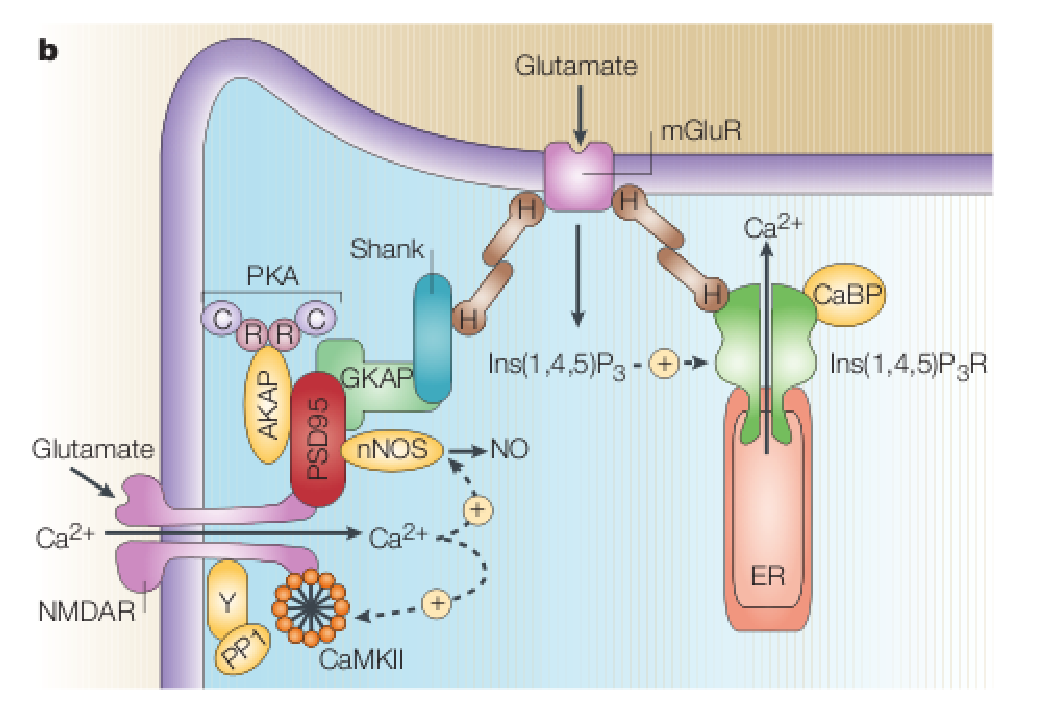
\includegraphics[height=8cm]{./images/NMDAR_complex.eps}}
  \caption{NMDAR links to other signalling components}\label{fig:NMDAR_complex}
\end{figure}

Hyperactivation of NMDAR leads to  neuropathological  states (such as brain
infarct formation during stroke). The classical view suggest this NMDAR
activity-dependent of neurophathological state required Ca2+ influx, which leads
to intracellular Ca2+ dysregulation  when  cytosolic  buffering capacity  is 
overwhelmed, or leading to mitochondria-dependent cell death.

However, applying NMDAR-blockers such as aptiganel (Cerestat)  show  little
neuroprotective  efficacy  in  clinical trials
(Sect.\ref{sec:NMDAR-antagonist}); while NMDAR-blocker via competing
Glutamate-binding shows promise  for  neuroprotection  though it was  poorly
tolerated because  of  adverse  cognitive  side effects.


Such recent evidence suggests signaling cascades in stroke initiated after
binding of NMDAR agonists may be distinct from those initiated by ion permeation
through open NMDAR channels. This is, for the first time, suggest the {\bf
metabotropic role of NMDAR}. Indeed, NMDARs, Src kinase and Panx1 form a
signaling complex, and activation of Panx1 required phosphorylation at Y308. 


\subsection{-- structure: NR1 and NR2 subunits}
\label{sec:NMDAR-structure}
\label{sec:NR2-NMDAR}
\label{sec:NR1-NMDAR}
\label{sec:NMDAR-isoforms}

The NMDA receptors are {\bf heteromeric assemblies} of two subunits NR1 and two
subunits of NR2. There is also a related gene family of NR3 subunit that once
added to the receptor, it has an inhibitory effect on the receptor activity
(Sect.\ref{sec:NR3-NMDAR}. \textcolor{red}{\bf NOTE: NR1, NR2, NR3 are used in
old nomenclature. Now, we should use GluN{\it x}{\it Y}} with {\it x}=1, 2, 3;
and {\it Y}=A, B, C.

{\bf NR1 and NR2 subunits}: Paoletti (2011)
\begin{itemize}
  \item  NR1 is the key subunit (GRIN1, GluN1) encoded by a single gene but has
  distinct 8 isoforms (due to RNA splicing): {\bf GluN1-1a to 4a; and GluN1-1b
  to 4b}.
 
 NOTE: {\bf b} isoforms contain an additional extracellular 21 a.a stretch (or
 N1 cassette) encoded by exon 5; and affect the receptor functional properties. 
 
  \item NR2 has 4 different subtypes: NR2A (GluN2A), NR2B (GluN2B), NR2C
  (GluN2C), NR2D (GluN2D).

NR2 subunit is an essential factor in the biophysical and pharmacological
properties of NMDA receptors, and can influence NMDA receptor assembly, ion
conductance (maximum conductance, decay time) and synaptic plasticity.


\end{itemize}

\subsection{-- structure: NR3 subunits}
\label{sec:NR3-NMDAR}

NR3 subunit is a related gene family that once added to the NMDAR
(Sect.\ref{sec:NMDAR-structure}), it has an inhibitory effect on the receptor
activity
 \begin{enumerate}
     \item NR3A subunit (GluN3A)
     \item NR3B subunit (GluN3B)
\end{enumerate}

GluN3 is thought to form either diheteromeric (GluN1/GluN3) or triheteromeric
(GluN1/GluN2/GluN3) (Traynelis et al., 2010). 


\subsection{-- subunit sequence}

\begin{verbatim}
NTD -- S1 -- M1  - M2(P-loop) -- M3 -- S2 -- M4 -- CTD
\end{verbatim}

A subunit in NMDAR typically consists 4 discrete domains separated by 4
trans-membrane domains (M1, M2, M3, M4) and two loops (S1, S2). NOTE: M2 is a
short re-entrain loop aka P-loop.
\begin{enumerate}
  \item extracellular region: a randem of large globular clamshell-like domain
  (NTD or N-terminal domain) of 380 a.a.
  
  NTD is related to leucine-isoleucine-valine binding protein (LIVBP) in
  bacteria
  
  \item agonist-binding domain (ABD) of around 300 a.a. which is formed by S1
  and S2 region
  
  ABD is related to glutamine-binding protein in
  bacteria.
  
  Glycine binds to GluN1 and GluN3; while Glutamate binds to GluN2.
  
  \item pore region 
  
  Pore region is similar to KCsA potassium channel in bacteria
  (Sect.\ref{sec:KcsA})
  
  \item C-terminal domain (CTD)
\end{enumerate}

\subsection{-- kinetics}
\label{sec:NMDAR-kinetics}

NMDAR is a receptor functioning as a non-selective ion channel. It means that
any ions (\ce{Ca^2+}, \ce{Na+}, \ce{K+}) can go through this ion channel.
Calcium flux through NMDARs is thought to play a critical role in synaptic
plasticity - the ability for the synapse to change its strength, a cellular
mechanism for learning and memory.

NMDAR is distinct in two ways: (1) it is both ligand-activated and
voltage-dependent; (2) it requires co-activation by different ligands.

\begin{enumerate}
  \item NMDAR has high $\Ca$ permeability than Glu2R-lacking non-NMDAR
  (Sect.\ref{sec:AMPAR-GluR1}).

  \item NMDAR is blocked by $\Mg$ which can be removed upon membrane
  depolarization (Sect.\ref{sec:NMDAR-Mg-block}) 
  
  \item Once $\Mg$ block is removed, activation of NMDAR requires glutamate,
  and co-agonist glycine (or D-serine) (Sect.\ref{sec:Glycine}).

As shown in Fig. \ref{fig:NMDAR}, its activation requires the binding
of {\it glutamate} or aspartate (aspartate does not stimulate as
strong as glutamate).

  \item NMDAR is subjected to (allosteric) modulation by extracellular
  compounds, i.e.
  NMDAR has modulatory sites for polyamines, reducing agents, $\Zn$ and protons. 
\end{enumerate}

\begin{figure}[htb]
  \centerline{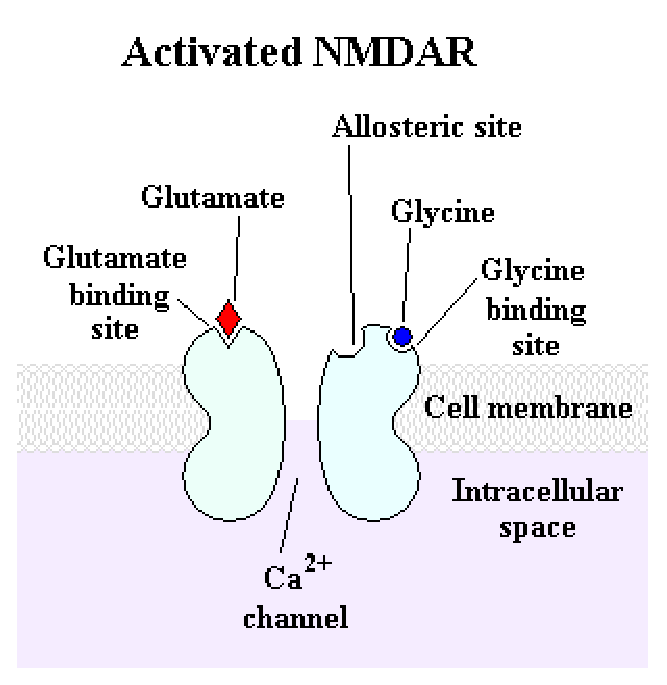
\includegraphics[height=6cm]{./images/activated_NMDAR.eps}}
  \caption{activated NMDAR }
  \label{fig:NMDAR}
\end{figure}


NMDAR has a slower kinetics than AMPAR, with a rise time of about 20 msec, and
two decay time constants (of about 25msec and 125msec at 32$^\circ$C)
\citep{hestrin1990}. The slow kinetics of activation is due to the requirement
of 2 agonist molecules binding to open the receptor, as well as a relatively
slow channel opening rate of bound receptors (Clements - Westbrook, 1991). The
slower decay term is believed to be due primarily to slow unbinding of glutamate
from receptor (Lester, Jahr 1992; Bartol-Sejnowski, 1993).

Opening probability $P_o$ reaches the peak about 0.3, suggesting the possibility
that saturation of synaptic NMDAR during high-frequency stimulus trains.

Recruitment of PKA and PP1 to NR1 subunit of NMDAR via AKAP9/yotiao.

NMDAR also associates with other proteins such as {\bf yotiao} (Y), which binds
PP1, and the scaffolding protein PSD95, which links to other signalling
components (AKAP-PKA complex, guanylate kinase-associated protein (GKAP)).

Proteins (shank and Homer (H)) might link the metrabotrophic glutamate
receptor (mGluR) to both NMDAR and IP3R, which is also associated with
a \ce{Ca^2+}-binding protein (CaBP).


\subsection{-- Magnesium block}

Magnesium block was first found in 1984 by Nowak et al. (1984) and Mayer et al.
(1984). Nowak et al. (1984) tested NMDAR on mesencephalic or striatal neurons in
13- or 15-day-old mouse embryos after being kept for culture for 6-10 days.

In $\Mg$-free solution
\begin{itemize}
  \item  membrane potential is held at (Vm = -60 mV), and apply 2-10 $\muM$
  glutamate, it elicited an inward current which remain stable over up to 10
  min. 
  
  This current varies nearly linearly with $\Vm$:
  \begin{equation}
  I_{\NMDAR, \text{no $\Mg$}} = g (\Vm - E_\rev)
  \end{equation}
  with $E_\rev$ is 0 mV at external $\Ca$ of 1mM (physiological condition). 
  The reversal potential is shifted at different external $\Ca$ concentration,
  in that increase $[\Ca]_e$ reduces single channel conductance.

  \item the mean open time of NMDAR is not a function of $\Vm$, and stay open
  for long period of time, showing the form of rectangular current pulses.
  
  The open time is nearly 5ms at 27$^\circ$C; and 3ms at 30$^\circ$C.
  This is NOT altered by $\Mg$ when $\Vm$ is in the positive potential range. 
   
  \item single-channel conductance is about 49$\pm$8 pS. 
\end{itemize}

In the presence of $\Mg$
\begin{itemize}
  
  \item single-channel current measured at resting potential are
  chopped in bursts of short opening separated by brief closures (Ascher,
  Nowak, 1988).
  
  This short mean open time is not a function of $[\Mg]_o$; but varies with
  membrane potential.
  
  \item $P_o$ is reduced

  \item The blocking effect increases with hyperpolarization; and decrease with
  depolarization, yet they are at different rates (Ascher, Nowak, 1988)
  \begin{enumerate}
    \item blocking rate is nearly 3x more sensitive to $\Vm$ than unblocking
    rate
    
    \item e-fold increase in blocking rate for 17mV hyperpolarization; while
    e-fold increase in unblocking rate needs 47mV depolarization.
  \end{enumerate}  
With 500 $\muM$ $\Mg$, it markedly reduce the inward current. 
   
\end{itemize}

\begin{mdframed}

At resting $V_m$, external $[\Mg]$ (at mM) is much higher than inside
($\muM$ range): Influx of $\Mg$ via NMDAR nevertheless block the channel
itself, as $\Mg$ ions bind tightly to the channel pore and prevent further
permeation.

The dislodge of $\Mg$ requires the depolarization of $V_m$ at sufficient (1)
amplitude, and (2) duration.

\end{mdframed}

\begin{itemize}

  \item Glycine (Sect.\ref{sec:Glycine}) is a required co-agonist along with
  (L-glutamate or aspartate) for NMDAR for efficient opening of the ion channel
  \citep{blanke2009}.

At holding potential -60mV of {\it Oocyte} (NOTE: resting potential is -64mV),
and $\Mg$-free,
\begin{enumerate}
  \item  application of 300$\muM$ NMDA elicited 
\begin{itemize}
  \item  a large inward current 66$\pm$13 nA in the presence of added 3$\muM$
  glycine which is 95\% of maximal response.
  
  \item a neglible current 0.6 $\pm$0.4 nA in the absence of added glycine
  
\end{itemize}

  \item application of 3.0 mM NMDA: produced a small current
  that does not change upon application of NMDAR-blocker, i.e. 1mM $\Mg$ or 100
  $\muM$ D-AP5
  
  Thus, high NMDA induces a current that is not due to activation of NMDAR
\end{enumerate}

The role of glycine was first observed in mouse brain, and then {\it Xenopus
oocytes}, and only affect on NMDAR, not for other receptors such as kainate
receptor (Sect.\ref{sec:kainate_receptor}) or quisqualate.
  
Recently, {\bf D-serine} has also been found to co-agonize with NMDAR with even
greater potency than glycine.  D-serine can be released both by neurons and
astrocytes to regulate NMDA receptors.
% TODO: check the role of D-serine


  
\end{itemize}
% two
% ligands (L-glutamate - Sect.\ref{sec:NMDA} and glycine - Sect.\ref{sec:Glycine}) .

\subsection{-- distribution}
\label{sec:NMDAR-distribution}

The changes as you will see below usually manifested as changes in the
kinetics and sensitivity to allosteric modulation. 
\textcolor{red}{``Classical'' NMDAR are those lacking GluN3.} 

{\bf GluN1} subunit: Paoletti (2009)
\begin{enumerate}
  \item ubiquitously expressed in CNS; from embryonic to adult
  
  However, there are developmental and regional variant on the subtypes of GluN1
  isoforms.
  
  \item {\bf adult rat brain}: GluN1-2 are widely expressed and abundant
  throughout brain.
  
  GluN1-1 : concentrate in most rostral structures (cortex and hippocampus)
  
  GluN1-4: principally express in more caudal structures (thalamus and
  cerebellum)
  
  GluN1-3: express only at very low levels
  
  \item GluN1-a: outnumber GluN1-b (with ratio 5:1) in forebrain; but is less
  (ratio 1:5) in cerebellum.
  
  GluN1-a express highly in all principal cell layers of hippocampus (dentate
  gyrus granule cells, CA1-3 layers).
  
  GluN1-b express largely restricted to CA3 layer.
  
  \item 
\end{enumerate}


{\bf GluN2} subunit: Paoletti (2009)
\begin{enumerate}
  \item the expression patterns change significantly in both time
  (developmental stages) and space (brain regions)
  
  \item {\bf embryonic rodent CNS}: only express GluN2B
  and GluN2D (exclusively found in
  diencephalon and brainstem). 
  This change completely during the first 2 weeks following birth.
  
  \item {\bf after birth}: GluN2A expression granually increases (and become
  abundantly express in entire CNS of adult); and
   
  NR2A subunit (GluN2A): found in thalamus with more prominent in lateral
  thalamic nuclei, especially ventrobasal complex
  \begin{enumerate}
    \item in striatum: more on lateral direction.
  \end{enumerate}
  
  \item GluN2B: after birth, GluN2B also increase but get peak around P7-P10 of
  postnatal days and also become restricted to forebrain areas (cortex,
  hippocampus, striatum, olfractory bulb).
  \begin{enumerate}
    %\item NR2B subunit (GluN2B):  found in thalamus
    \item uniform throughout striatum
    
    \item 
  \end{enumerate}
   
  \item GluN2C: after birth, at P7, GluN2C starts to appear with expression
  mainly confined to {\bf cerebellum} (granulle cells) and olfactory bulb. 
    
  NR2C subunit (GluN2C): express a high level in cerebellum, but low
  elsewhere.
  
  \item GluN2D: GluN2D drops markedly after birth; and in adult, GluN2D subunits
  is weakly expressed in diencephalon and brainstem.
   
  NR2D subunit (GluN2D): express early during development rather than in
  the adult.
    
\end{enumerate}


{\bf GluN3} subunit: Paoletti (2009)
\begin{enumerate}
  \item GluN3A: low before birth; and peaks during early postnatal life (maximal
  at around P8); then start to decrease to low levels in adulthood.
  
  \item GluN3B: express at low level in early stages after birth; and increase
  progressively until peak in adulthood.
  
  GluN3B was initially thought to be restricted in brainstem and spinal cord; it
  is now accepted as ubiquitous in CNS.
  
\end{enumerate}

\subsection{-- ionic current}

Much of the calcium entering the postsynaptic spine comes through NMDA
receptors. Blocking NMDA receptors pharmacologically can eliminate both LTP and
LTD (Sect.\ref{sec:LTplasticity}), and a partial block of NMDA receptors can
convert an LTP protocol to LTD \citep{blanke2009}.

NMDAR has the special property of allowing calcium to enter the postsynaptic
spine only when presynaptic activation and postsynaptic depolarization occur at
the same time.

\begin{enumerate}  
  \item NR2A  confers a lower affinity for both glutamate and NMDA, distinctly faster
kinetics and higher channel open probability than does the NR2B subunit.

NR1-NR2A receptor differs from others in its response to reducing agents
  
  \item NR2B confers slower channel kinetics and reduced open probability
    
  \item NR1-NR2C receptor are more sensitive to $\Mg$ block and display highest affinity
sites for glycine binding compared to other heteromeric channels
    

\end{enumerate}
 
\subsection{-- agonist/antagonist}
\label{sec:NMDAR-antagonist}

NMDARs are important therapeutic targets for many CNS disorders including
stroke, hypoxia, ischemia, head trauma, Huntington's
(Sect.\ref{sec:Huntington-disease}), Parkinson's, and Alzheimer's diseases,
epilepsy, neuropathic pain, alcoholism, schizophrenia, and mood disorders. To
date, drugs targeting NMDARs have had only limited success clinically due to
poor efficacy and unacceptable side effects, including hallucinations,
catatonia, ataxia, nightmares, and memory deficits.

Most NMDA receptor antagonists are metabolized in the liver.
Frequent use of most NMDAR antagonist can lead to tolerance due to liver
obsorbing these NMDAR antagonist more quickly from the bloodstream.

NMDAR blockers (NMDAR antagonists) can be competitive or uncompetitive:
\begin{itemize}
  
  \item mild blockage: amitriptyline 
  
  \item competitive

NMDAR can be antagonised in a competitive manner by substituted 5-carbon and
7-carbon chain glutamate analogues such as
\begin{enumerate}
  \item APV = D-2-amino-5-phosphonovaleric
  
  \item D-AP5 = D-2-amino-5-phosphonopentanoate, e.g. 40$\muM$

  \item AP5 = DL-2-Amino-7-phosphonoheptanoic acid 

  \item CPP = 3-(($\pm$)-2-carboxypiperazin-4-yl)-propyl-1-phosphonate
  
  \item selfotel:  block NMDAR by competing with glutamate, i.e. acts  at 
  the ligand-binding site for glutamate.
  
\end{enumerate}

  \item  uncompetitive: 
\begin{enumerate}
  \item Ketamine: has shorter half-life and lower potency than MK-801
  
  \item dextromethorphan (DXM), 
  
  \item phencyclidine (PCP), 
  
  \item methoxetamine (MXE), and
   
  \item nitrous oxide (N2O)

  \item MK-801 (Dizocilpine): block regardless of the subunit composition of the
  channel. 
  
  MK-801 (MK801) is classically applied in the external medium to block NMDAR.
  Recent evidences showed that it can be used intracellularly - i-MK801 (Bender
  et al.
  2006, Nevian and Sakmann, 2006). As it is an open channel blocker, $0-\Mg$
  extracellular solution should be used to improve the efficiency of NMDA
  channel block by i-MK801.
  
  It inhibits the extracellular signal-regulated kinase 1/2-signaling cascade -
  an intracellular signaling cascade that is activated by growth factors and
  controls the proliferation of cancer cells
  
  It reduces the phosphorylation of cAMP-responsive element binding protein,
  suppresses the expression of cyclin D1, up-regulates the cell cycle regulators
  and tumor suppressor proteins p21 and p53, and increases the number of lung
  adenocarcinoma cells in the G2 and S phases of the cell cycle.
  
  \end{enumerate}

  \item aptiganel (Cerestat): use-dependent NMDAR open channel blockers 

\end{itemize}
\url{http://en.wikipedia.org/wiki/NMDA_receptor_antagonist}


\subsection{NMDA/AMPA current ratio}
\label{sec:NMDA-AMPA-current-ratio}

NMDAR (Sect.\ref{sec:NMDAR}) and AMPAR (Sect.\ref{sec:AMPAR}):

Because these receptors have distinct kinetics (AMPA, 2-7 ms; NMDA,   50-100 ms)
and because the NMDA receptor is important for $\Ca$-dependent plasticity
and learning, the ratio of NMDAR/AMPAR current at excitatory synapse is likely
to be a key determinant to both short-term integration and long-term
modification of synaptic inputs in rat \citep{myme2003}. 
\begin{enumerate}
  
  \item layer 5 visual cortex (VC), 0mM $\Mg$: peak NMDA/AMPAR is 220
  
  \item layer 5 s.s. cortex, 2mM $\Mg$: peak NMDA/AMPAR is 30
  
  \item  layer 3, 2mM $\Mg$: peak NMDAR/AMPAR is 20
  
  \item layer 4 barrel cortex,  0mM $\Mg$: peak NMDAR/AMPAR is 86$\pm 64$
  
  \item 
  
  \item visual cortical synapse {\it in vitro}: shows a constant NMDAR/AMPAR
  current ratio [Watt et al. 2000]
  
  
  
  \item layer 2/3 prefrontal cortex (PFC) and visual cortex (VC) 
  pyramidal cells in rat aged p16-p21 (no difference with recordings in older
  rat p26-p29):
  
  {\bf mEPSC condition} (at 0mM $\Mg$ extracellular): the NMDA/AMPA ratio is 27
  (in PFC), and 28 (in VC); mEPSC is well-fitted by double exponentials with
  peak mESPC amplitude (PFC:  19.1$\pm$1 pA; VC: 17.5$\pm 0.5$ pA), NMDA decay
  kinetics $\tau$ (PFC:  $69\pm 8$ ms; VC: $67\pm 6$ ms)
  
  {\bf evoked EPSC condition} (at 2mM $\Mg$ extracellular): the NMDA/AMPA ratio
  increase in both regions, but still the same (PFC, VC: 109).
  
NOTE: By around p28, many other properties of cortical synapses have largely
matured in rat.

  \item striatal: 
  
  
  the major components of the striatal glutamate receptors are GluR2-containing
  AMPA receptors and NR2A-containing NMDA receptors
  
  
\end{enumerate}

The NMDAR is a favored candidate mechanism for {\bf sustained recurrent
excitation} because the slow kinetics aid stability of the memory trace, and the
dual activation requirements of depolarization and ligand binding could be used
to select a reverberating circuit of only those cells which receive an initial
stimulus

\citep{myme2003} suggested the function of AMPARs and NMDARs are regulated
similarly in the supragranular layers of two functionally distinct cortical
regions, suggesting a homogeneity of regulation of these receptors across the
cortex. Therefore, the regional specification may be accounted by other factors,
such as inputs, modulation, and circuitry.


The subunits of NMDAR and AMPAR play a critical role to the receptors's
physiological function. However, the composition of the NMDA and AMPA receptor
subunits has not been well established using electrophysiological methods in the
dorsal striatum. \citep{jeun2009} did a study on this

\subsection{presynaptic iGluR}
\label{sec:iGluR-presynaptic}




\section{-- mGluR: metabotropic glutamate receptors}
\label{sec:mGluR}
\label{sec:metabotropic-GluR}

{\bf Metabotropic glutamate receptors} (mGluR) are members of the {\bf group C
family of G-protein-coupled receptors} with extracellular N-terminal,
intracellular C-terminal and 7 TMs (Sect.\ref{sec:G-protein-coupled-receptor}).
The first evidence of glutamate receptors that are not ligand-gated cation
channels - mGluR - was published in mid to late 1980s. Rather than permeating
ions, mGluR activate biochemical cascades, leading to the modification of other
proteins, e.g. other ion channels.

Like all glutamate receptors (Sect.\ref{sec:glutamate_receptor}), mGluRs is
activated upon either 
\begin{itemize}
  \item glutamate binding - an amino acid that functions as an
excitatory neurotransmitter

  \item N-Acetylaspartic acid - Sect.\ref{sec:NAA}
\end{itemize}.

% They modulate postsynaptic ion channels indirectly, differ in their coupling
% to intracellular messengers and in their sensitivity to pharmacological
% agents.

There are 8 different types of mGluRs: mGluR1 to mGluR8 (GRM1 to GRM8), divided 
into 3 groups: I, II and III. 
\begin{enumerate}
  \item class I (Sect.\ref{sec:mGluR_group-1}): mGluR1, mGluR5, and their
  respective splice variants.
  
\textcolor{red}{Activate: PLC}
  
  \item class II (Sect.\ref{sec:mGluR_group-2}): mGluR2, mGluR3

Other members: {\it Drosophila mGluR} (DmGluRA)
  
\textcolor{red}{Deactive: AC}
  
  \item class III (Sect.\ref{sec:mGluR_group-3}): mGluR4, mGluR6, mGluR7, mGluR8

\textcolor{red}{Deactive: AC}

The mGluRs are further divided into subtypes, such as mGluR7a and mGluR7b.
\end{enumerate}
Other members: bovine parathyroid $\Ca$-sensing receptor (PCaR) (also activate
PLC) : though not belong to any of the three groups; with least sequence
similarity.

\subsection{Localization}
%\subsection{-- group I}
\label{sec:mGluR_group-1-distribution}
\label{sec:mGluR_group-2-distribution}
\label{sec:mGluR_group-3-distribution}

\textcolor{red}{\bf Distributions}: All mGluRs except mGluR6 are thought to
exist in the hippocampus and entorhinal cortex.

\begin{enumerate}
  \item Group I mGluR (mGluR1/5) - Sect.\ref{sec:mGluR_group-1}:
    \textcolor{red}{found mainly in post-synapse} in an area known as
    postsynaptic density (PSD) at excitatory synaptic sites.

mGluR1 staining is most intense in Purkinje cells of the cerebellar cortex and
mitral/tufted cells of the olfactory bulb.  Strong expression is also observed
in neurons of the lateral septum, the pallidum and in the thalamus (Luscher, Huber, 2011)


Unlike mGluR1, mGluR5 is observed in the cerebral cortex, hippocampus,
subiculum, olfactory bulb, striatum, nucleus accumbens and lateral septal
nucleus. In the hippocampus, mGluR5 is mainly expressed in dendritic fields of
the stratum radiatum, whereas mGluR1 is mostly found on cell bodies (Luscher,
Huber, 2011).

The metabotropic glutamate receptor mGluR5, but not the closely related mGluR1,
is expressed in cultured astrocytes, and this expression is up-regulated by
specific growth factors (Nakahara, Okada and Nakanishi, 19997).

  
  \item Group II :   (mGluR2/3) which are enriched both presynaptically and
postsynaptically
  
%\textcolor{red}{found mainly in post-synapse}  
  
  \item Group III: 
  group III mGluRs (mGluR4/6/7/8) which are usually predominant presynaptically
%  \textcolor{red}{found mainly in post-synapse}

mGluR4 is located only in the brain, in locations such as the thalamus,
hypothalamus and caudate nucleus.   
\end{enumerate}

\subsection{agonists (3 groups)}
\label{sec:mGluR_group-1-agonist}

\textcolor{red}{\bf Activators} (agonists):
(1S,3R)-1-aminocyclopentane-1,3-dicarboxylate (1S,3R-ACPD) is mGluR-selective
agonist.

\begin{enumerate}

  \item Group I mGluRs:
  
{\bf specific agonist}: DHPG (3,5-dihydroxyphenylglycine) - agonist to mGluR
group I (mGluR1 and mGluR5), so group I mGluR can be isolated for studies easily.

$30\muM$ DHPG can elicits a robust increase in fluorescence in CA1 pyramidal cells
that were loaded with the calcium-sensitive dye fluo-3 in both soma and
dendrites \citep{mannaioni2001}

{\bf non-specific agonist}: {\it t-ACPD} is a nonspecific mGluR-I agonist.

  
  \item Group II mGluRs:
  
2R,4R-APDC; 2-(2,3-dicarboxycyclopropyl)glycine (DCG-IV) and eglumegad.
  
NOTE: Biphenylindanone A only activate mGluR2.
  
  \item Group III mGluRs:
  
2-amino-4-phosphonobutyrate (L-AP4).

\end{enumerate}


\subsection{blockers (antagonist)}
\label{sec:mGluR_group-1-antagonist}

\textcolor{red}{\bf Blockers}:
\begin{enumerate}
  
  \item Group I mGluR: 
  
  {\bf mGluR1 blocker}: potent competitive antagonist selective for mGluR1
  ((S)-(+)-$\alpha$-amino-a-methylbenzeneacetic acid (LY367385), e.g.
  200$\muM$ in pipette);  7-(hydroxyimino)cyclopropa[b]chromen-1a-carboxylate
  ethyl ester
  
  
  {\bf mGluR5 blocker}: potent noncompetitive antagonist that is selective for
  mGluR5 (2-methyl-6-(phenylethynyl)-pyridine (MPEP), e.g. 100$\muM$ in pipette)
  
  \item Group II mGluR:  selective antagonist blocking (LY341495 and
  MGS-0039),   negative allosteric modulator (RO4491533)

\end{enumerate}
\url{http://en.wikipedia.org/wiki/Metabotropic_glutamate_receptor}

\subsection{class I: mGluR1, mGluR5}
\label{sec:mGluR_group-1}

The class I mGluR (group I) receptors are found in postsynapse in an area known
as   postsynaptic density (PSD) at excitatory synaptic sites; and thus involve
into postsynapse activity \citep{lujan1996, mao2008}.  Group 1 mGluRs are
comprised of mGluR1 and mGluR5, and splice variants
\begin{enumerate}
  \item 6 mGluR1 splice variants (1a or 1$\alpha$, 1b or 1$\beta$, 1c, and 1d)
  
  \item 2 mGluR5 splice variants (5a and 5b),
\end{enumerate}
Only the long-form group I mGluR (1a, 5a, and 5b) has the C-terminal.
The distribution of each type is mentioned in
Sect.\ref{sec:mGluR_group-1-distribution}. The receptor links to G$\alpha$q/11
heterotrimeric G-proteins (Sect.\ref{sec:Gq/11-protein}).



\begin{enumerate}
  \item  MSNs in the striatum express mainly the group-I mGluRs (mGluR1,5)
  (Testa et al.   1994).

  They do not express detectable levels of mGluR1 but express widely mGluR5 in
  the somatodendritic elements (Uchigashima et al. 2007)

  \item Purkinje cells:
  
NOTE: Quantitative single-cell RT-PCR analysis (Sect.\ref{sec:scRT-PCR}) showed
that Purkinje cells express at least 10-fold more Gq$\alpha$ than G11$\alpha$.
This explains the dominant role of Gq in Purkinje cells
(Sect.\ref{sec:Gq/11-protein}).
  
\end{enumerate}


\subsection{-- pathogenesis}

\textcolor{red}{\bf Pathogenesis}:
\begin{itemize}
  \item neurotoxicity: due to overactive of NMDAR

Since mGluRs and ionotropic glutamate receptors are co-clustered in the localized PSD of
excitatory synapses, a reciprocal regulation between them vigorously occurs in response to
changing synaptic inputs. Activation of mGluR1/5 enhances NMDA receptor function, one of
the most prominent effects of active mGluR1/5 in a number of brain regions (Fitzjohn et al.,
1996; Benquet et al., 2002; Heidinger et al., 2002; Kotecha et al., 2003; Huang and van den
Pol, 2007). Similarly, activation of NMDA receptors potentiates mGluR5-mediated responses
(Lüthi et al., 1994; Challiss et al., 1994; Yang et al., 2004). 
Such positive crosstalk is important
for organizing diverse forms of synaptic plasticity and contributes to the pathogenesis of
various mental and neurodegenerative illnesses. 

NMDA at low (5-15 $\muM$), but not high (50-100 $\muM$), concentrations enhanced
mGluR5 responses through activation of a PP, followed by dephosphorylation of
PKC phosphorylation sites on mGluR5 (such as S890) and thereby reduction of
PKC-mediated desensitization


Prolonged neuron excitation by glutamate and ion influx can be toxic to neurons.
This excitotoxicity effect is a main cause of neuronal death in stroke and CNS trauma.
  
  \item development of certain types of cancer: mutatation in mGluR1 in mice
  
  \item Fragile X, a type of autism: 
  
  studies to find potential of drugs that modify class I mGluR in
  helping development of the treatment for Fragile X.
  
\end{itemize}

\subsection{-- function}

mGluR1 is a member of mGluR group I (Sect.\ref{sec:mGluR_group-1}).
Its distribution is mentioned in Sect.\ref{sec:mGluR_group-1-distribution}.

The activation of mGluR gorup I links to:
\begin{enumerate}
  
  \item {\it classic signal transduction}: There are two types of G$\alpha$
  subunits associated with class I mGluR (G$\alpha$q and G$\alpha$11).
  
  Upon mGluR group I activation by selective agonist
  (Sect.\ref{sec:mGluR_group-1-agonist}), it releases the two G-protein subunits
  which lead to several signaling cascades - Sect.\ref{sec:Gq/11-protein}.
  
  
   \item {\it other signal transductions}: production of cAMP and arachidonic
   acid, as well as a link to inhibiting voltage-dependent N-type $\Ca$ channels
   and $\Ca$-dependent K+ channels, $I_\AHP$, M-current $I_M$ 
   \citep{anwyl1999}
   
   \item {\it affect doparminergic and adrenergic neurotransmission}
\end{enumerate}

Even though both mGluR1 and mGluR5  both trigger the release of Ca2+ from
intracellular stores via IP3R, they induce different response patterns of $\Ca$
patterns
\begin{enumerate}
  
  \item  mGluR1a activation induced a single-peaked Ca2+ rise; while mGluR5a
  activation elicited characteristic Ca2+
 oscillations

\textcolor{red}{\bf In lamprey locomotor network} (Kettunen et al., 2002):
In expression systems, mGluR1 elicits a single-peaked nonoscillatory [$\Ca$]i
response, whereas mGluR5 elicits oscillations (Kawabata et al., 1996; Nakanishi
et al., 1998); and an activation of native mGluR5 in neurons
induces different cellular effects. 

In hippocampus neurons, mGluR5 elicits a singlepeaked [$\Ca$]i response (Rae et
al., 2000), whereas it induces [$\Ca$]i oscillations in the neocortex (Flint et
al., 1999). 

    \item mGluR5a activation elicited characteristic Ca2+
 oscillations require phosphorylation at a single amino acid (Kawabata et al.,
 1996; Uchino et al., 2004 ; Kim et al., 2005 ; but Dale et al., 2001) -
 Sect.\ref{sec:mGluR_group-1-phosphorylation}.
    
    
Activation of mGluR5 induces [$\Ca$]i oscillations that do not require protein
kinase C (PKC) activation, but depend on $\Ca$ entry through L-type channels. 
  
   \item mGluR5 potentiate NMDAR 
   
In neurons of the subthalamic nucleus, mGluR5 potentiates NMDA receptor currents
(Awad et al., 2000).


In lamprey spinal cord neurons the two subtypes of group I mGluRs have different
cellular effects; mGluR1 potentiates NMDA receptors and mGluR5 induces [$\Ca$]i
oscillations (Kettunen et al., 2002).

\end{enumerate}

\subsection{-- modulator (phosphorylation)}
\label{sec:mGluR_group-1-phosphorylation}

There are evidences of mGluR phosphorylation in heterologous cells and brain
cells (Kim et al., 2008) - Sect.\ref{sec:phosphorylation} which can enhance
(e.g. by tyrosine kinase) or desensitize the receptor (e.g. by PKC) (review:
Mao et al., 2008).

% In the case of crosstalk between NMDAR and mGluR5, NMDAR could potentiate
% mGluR5 function through either enhancing tyrosine phosphorylation or
% inhibiting PKC phosphorylation or both.

There are two forms of desensitization (i.e. reduce affinity to agonist) caused
by phosphorylation: homologous (agonist-dependent) and heterologous
(agonist-independent) desensitization of the receptor (Dhami and Ferguson, 2006).
\begin{itemize}
  \item  stimulation of mGluR1/5 with the selective agonist leads to the DAG-
dependent activation of PKC

Activated PKC can then phosphorylate mGluR1/5 to promote the homologous type of
desensitization, an attenuation of receptor responsiveness to repeated or
prolonged agonist stimulation (Lefkowitz, 1993).

This has been found in cultured neurons (Catania et al., 1991 ; Aronica et al.,
1993) or Xenopus oocytes expressing mGluR5a (Gereau and Heinemann, 1998).
 

  \item PKC activators induced a desensitization-like reduction of mGluR1/5
  signaling in hippocampal slices (Schoepp and Johnson, 1988) or Xenopus
 oocytes (Gereau and Heinemann, 1998)

Protein kinase A (PKA) selective agents (an activator or inhibitor) had no
effect on the desensitization (Gereau and Heinemann, 1998).

  \item heterologous desensitization since PKC inhibitors blocked the group I
  mGluR desensitization induced by stimulation of heterologous G$\alpha$
  q/11-coupled muscarinic M1 receptors (Mundell et al., 2002; 2004).


\end{itemize}


NOTE: CaMKII, conventional PKC ( $\alpha$ , $\beta$ , $\gamma$ ), and CaM are
all Ca 2+ -sensitive molecules.
Significant crosstalk among them is believed to occur for the sake of
sophisticatedly coordinating mGluR1/5 responses to changing signals from
glutamatergic synapse.

\begin{enumerate}
  \item PKC - Sect.\ref{sec:PKC} at serines/thereonine sites

PKC phosphorylation of mGluR1/5 is believed to disrupt normal G protein-coupling
and thereby reduce the efficacy of mGluR1/5 signaling.
In mGluR1a threonine residue (T695; T681 in mGluR5a) that is involved in the
receptor coupling to G$\alpha$q/11 (Francesco and Duvoisin, 2000); and mutation
of this residue almost completely abolished mGluR1$\alpha$-mediated rapid
desensitization. T695 (mGluR1a) or T681 (mGluR5a) is located within a hinge
region of the second intracellular loop, and is found only in group I mGluR.
  
Mutation of multiple sites in the first and second intracellular loops and the
C-terminus of mGluR5a (T606, S613, T665, S881, and S890) seems to be sufficient
to block the PKC-dependent desensitizationmutation of multiple sites in the
first and second intracellular loops and the C-terminus of mGluR5a (T606, S613,
T665, S881, and S890) seems to be sufficient to block the PKC-dependent
desensitization. PKC is thought to phosphorylate these residues to inhibit the
receptor function, although actual phosphorylation status of these sites was not
tested in this model. Interestingly, the T840 that is essential for generating
the oscillatory Ca2+ responses to mGluR5 activation had no functional impact to
the desensitization of mGluR5 ( Gereau and Heinemann, 1998).
  
PKC activator mimicked the effect of the mGluR1/5 agonist in phosphorylating
mGluR1c (Ciruela et al., 1999); and agonist-induced phosphorylation could be
abolished by a specific PKC inhibitor Ro318220 (Alaluf et al., 1995).

Later on,  PKC-mediated phosphorylation site at rat mGluR5a in heterologous
cells: a threonine residue at position 840 (T840) within the proximal region of
mGluR5a C-terminal tail, a region also harboring G proteins (Kawabata et al.,
1996); with likely by the Ca2+ -independent PKC $\delta$ isoform rather than
Ca2+ - dependent PKC $\gamma$) - Sect.\ref{sec:PLC-gamma} (Uchino et al., 2004).
A recent study suggested the Serine 839 (S839) is probably the real residue at
which phosphorylation occurs while the adjacent T840 only plays a permissive
role in the PKC- dependent phosphorylation of S839 (Kim et al., 2005).
However, the permissive role of T840 is unique to mGluR5a since this site is not
conserved in mGluR1a (D854). As a result, PKC did not phosphorylate the same
site at mGluR1a despite that S839 is conserved in mGluR1a (S853) (Kim et al.,
2005).


Other PKC- sensitive serine/threonine site(s) are believed to exist
because a truncated mGluR5 peptide lacking T840 still displayed the PKC-mediated
phosphorylation in vitro (Minakami et al., 1997).
Multiple PKC consensus phosphorylation sites (K/RxXS/T) (Pearson and
Kemp, 1991) can be found on intracellular regions of mGluR5a, including the first and second
intracellular loops in addition to the C-terminus

  \item $\Ca$-sensitive Calmodulin:
  
PKC-mediated phosphorylation described above can be regulated by calmodulin
(CaM). Ubiquitous CaM has been found to directly bind to two distinct sites on
the C-terminus of human mGluR5 (H845-L875 and W884-S936) which seem to have
different affinities for CaM (Minakami et al., 1997).
Such binding to either site was Ca2+-dependent and was able to inhibit the
PKC-mediated phosphorylation of mGluR5 ( Minakami et al., 1997).

Conversely, the PKC phosphorylation antagonized the binding of CaM to
mGluR5. Thus, PKC and CaM can reciprocally regulate each other's binding to mGluR5 to
accurately control phosphorylation of the receptor.

NMDA treatment increased the level of tyrosine phosphorylation of mGluR5
(Orlando et al., 2002) contrast to reduced PKC phosphorylation of the receptor
in response to NMDA (Alagarsamy et al. 1999; 2002).

  \item tyrosine kinases,
  
In addition to serine and threonine, tyrosine phosphorylation could occur to
mGluR1/5. Tyrosine phosphorylation supports mGluR5 function as opposed to the
inhibitory regulation of it by PKC-mediated phosphorylation.
PKC-mediated phosphorylation is specific to mGluR group I; while tyrosine
phosphorylation is not.

The protein tyrosine kinase inhibitors inhibited the mGluR1/5 response to the
agonist DHPG (Tozzi et al., 2001 )

In striatal neurons in vivo and in vitro (Orlando et al., 2002), mGluR5 was
tyrosine phosphorylated while no tyrosine phosphorylation of mGluR1a was
detected.

Tyrosine phosphorylation of mGluR5 was enhanced by the tyrosine phosphatase
inhibitor pervanadate, indicating the receptor is normally subject to an active
endogenous cycle of phosphorylation and dephosphorylation.

Tyrosine phosphorylation level of mGluR5 is positively correlated to the
efficacy of receptor signaling as the tyrosine phosphatase inhibitor produced
parallel increases in tyrosine phosphorylation and mGluR5-mediated PI hydrolysis
(Orlando et al., 2002)

GRK2 may also play a role in PKC- and CaMKII-mediated desensitization of group I mGluRs
as these enzymes seem to trigger GRK2 to associate with mGluR1a to promote an
internalization and desensitization of mGluR1a homologously induced by glutamate or
heterologously induced by an M1 agonist (Mundell, 2004)

  \item Ca2+/calmodulin-dependent protein kinase II (CaMKII):
  
CaMKII has been shown to phosphorylate and regulate a large number of receptors
and proteins at excitatory synapses (Yoshimura et al., 2002).
Given the co-clustering of CaMKII and mGluR1/5 at the defined PSD microdomain,
mGluR1 and/or 5 situate well as a substrate of CaMKII.

Available data so far obtained from pharmacological studies indicate that CaMKII
like PKC actively regulates mGluR1a. CaMKII activation is required for the
internalization and homologous desensitization of mGluR1a in response to
glutamate stimulation (Mundell, 2004). Similarly, active CaMKII contributes to
the internalization and heterologous desensitization of mGluR1a in response to
stimulation of muscarinic M1 receptors (Mundell et al., 2002; 2004).
  
CaMKII is an attractive serine/threonine kinase. CaMKII is highly abundant in brain cells, especially at synaptic
sites (Kelly et al., 1984). 
The activated kinase accesses and phosphorylates not only exogenous
substrates but also its autophosphorylation site (T286 in the 
$\alpha$ isoform). 

This renders and sustains a partial Ca 2+ /CaM-independent (autonomous) kinase
activity even after the initial Ca 2+
 stimulus subsides (Hudmon and Schulman, 2002; Colbran and Brown, 2004). As
 such,
CaMKII is capable of integrating information conveyed by diverse forms of local
Ca 2+ transients in a relatively long period of time

GRK2 may also play a role in PKC- and CaMKII-mediated desensitization of group I mGluRs
as these enzymes seem to trigger GRK2 to associate with mGluR1a to promote an
internalization and desensitization of mGluR1a homologously induced by glutamate or
heterologously induced by an M1 agonist (Mundell, 2004)
  
  \item  G protein-coupled receptor kinases (GRKs), 
  
  
Several members of the GRK family (GRK1-7), including GRK2, GRK4, and GRK5, may
phosphorylate mGluR1a. (Sect.\ref{sec:GRK}).

Constitutive and/or agonist-stimulated mGluR1a phosphorylation was enhanced by
co-expression of GRK2 (Dale et al., 2000) or GRK4 (Sallese et al., 2000 ) in
HEK293 cells.

GRK2, GRK4, and GRK5 have all been shown to contribute to
mGluR1 desensitization in heterologous or Purkinje cells (Dale et al., 2000;
2001; Sallese et al., 2000; Iacovelli et al., 2003).

However, the GRK2-mediated phosphorylation is not required for the
GRK2-dependent mGluR1a desensitization, but rather GRK2 desensitizes the
receptor by the direct binding to the receptor through its regulator of G
protein signaling (RGS) homology (RH) domain (Dhami et al., 2002 ; Dhami and
Ferguson, 2006).

Finally, mGluR5, like mGluR1a, can also be regulated by GRK2 in a kinase
activity-dependent manner (Sorensen and Conn, 2003 ). The T840 site in the
mGluR5a C-terminus appears to be at least partially important for the GRK2
regulation of mGluR5 function.

  \item and PPs - Sect.\ref{sec:PP-protein-phosphatase}: calcineurin
  (Sect.\ref{sec:calcineurin}).
  
The significant influence of PPs on mGluR1/5 phosphorylation suggests close
vicinity or likely direct physical interactions between the two proteins.
It is currently unknown whether other PP isoforms (PP1/2A, PP2B, etc.) can
directly bind to mGluR1/5.

Indeed, PP1$\gamma$1 (PP1C1) in both recombinant and native forms binds to the
C-terminus of long-form group I mGluRs, i.e., mGluR1a, mGluR5a, and mGluR5b
(Croci et al., 2003). The fact that the PP1$\gamma$ 1-binding motif on mGluR1/5
falls within or immediately distal to possible PKC phosphorylation sites (such
as S881 and S890 on mGluR5a) is noteworthy.

  
The regulation of protein phosphorylation requires coordinated interactions between protein
kinases and PPs. Phosphorylation of mGluR1/5 is therefore reasoned to be
regulated by PPs.

Application of okadaic acid, an inhibitor relatively selective for the
serine/threonine phosphatase PP1/2A, prevented the recovery of mGluR5a from
desensitization.

PP2A also forms complexes with mGluR5 in neurons in vivo
 based on the data from coimmunoprecipitation (Mao et al., 2005a).

PP is the link between NMDAR and mGluR5.
Alagarsamy et al. (1999; 2002) discovered a role of PPs. NMDA at low (5-15 $\mu$M),
but not high (50-100 $\mu$M), concentrations enhanced mGluR5 responses through
activation of a PP, followed by dephosphorylation of PKC phosphorylation sites
on mGluR5 (such as S890) and thereby reduction of PKC-mediated desensitization.
PP2B selective inhibitor cyclosporine-A blocked the effect of NMDA on
mGluR5-mediated responses.
  
An mGluR5 mutant (S890G), a form of the receptor resistant
to PKC-mediated desensitization, showed the lack of desensitization and the potentiating effect
of NMDA. 

Noticeably, the effect of NMDA was insensitive to okadaic acid (Alagarsamy et
al., 1999 ). This suggests an interesting scenario that the phosphatase
responsible for the effect of NMDA may be a phosphatase (likely PP2B, also known
as calcineurin) different from the okadaic acid-sensitive phosphatase (likely
PP1/2A) responsible for natural recovery of mGluR5 from desensitization (Gereau
and Heinemann, 1998).
  
\end{enumerate}



\subsection{- mGluR1}
\label{sec:mGluR1}


Activation of mGluR1
\begin{enumerate}
  \item induce increase postsynaptic $[\Ca]_i$ + direct depolarization of CA1
  hippocampal neuron (via blocking leak $\K$ current)
 
  
  $30\muM$ DHPG induces depolarization $\Delta V_m = 4.2\pm 0.3$ mV on CA1
  pyramidal cells, and was blocked completely by 100$\muM$ LY367385 
  ($\Delta V_m = 1.2\pm 0.1$ mV).
  
   There are different hypothesis for membrane potential increase, i.e.
  increasing inward current (as above), (1) inhibit the leak $\K$ current, (2)
  increase non-selective cationic conductance. However, as DHPG-induced inward
  current is associated with a decrease in membrane conductance (i.e. increase
  resistance), it suggest the underlying mechanism is inhibiting the leak $\K$
  conductance.
   
   \item (at GABAergic synaptic site) increase the frequency of spontaneous
   IPSCs (sIPSCs) of   inhibitory interneurons (Sect.\ref{sec:IPSC})
 
  it means increases firing of inhibitory interneurons, but at the same time (4)
  reduces the amplitude of evoked IPSC - \textcolor{red}{this suggest the reduction of
  evoked IPSC is mediated by pre-synaptic action (which suggest mGluR1 in
  presynaptic region) which is drived through
  {\bf hippocampal circuit}}, i.e. presynaptic mGluR1 activation can lead to
  presynaptic inhibition.
  \textcolor{red}{This is shocked as earlier data showed that mGluR5 is more abundant.}
 
  
  \item inhibit of transmission at the Schaffer collateral $\rightarrow$ CA1
  synapse
  
  
\end{enumerate}
\citep{mannaioni2001}

Evidence: DHPG-induced those changes above is blocked by using
mGluR1 blocker - LY367385.




\subsection{- mGluR5}
\label{sec:mGluR5}

mGluR5 is a member of mGluR group I (Sect.\ref{sec:mGluR_group-1}). Its
distribution is mentioned in Sect.\ref{sec:mGluR_group-1-distribution}.

mGluR5 has been implicated in switching from NR2B- to NR2A-containing NMDA
receptors, in both the hippocampus and visual cortex (Matta et al., 2011) -
Sect.\ref{sec:NMDAR}.

Activation of mGluR5
\begin{enumerate}
  \item suppress $\Ca$-activated potassium current $I_\AHP$
  (Sect.\ref{sec:SK_current}) in CA1 hippocampal neuron

  $30\muM$ DHPG binding mGluR5 suppressed $I_\AHP$ in a reversible manner in CA1
  pyramidal neuron.
  
   \item potentiate NMDAR

  increase peak NMDAR current by fast local application of
  100$\muM$ NMDA: Proteins called {\it PDZ proteins}
frequently anchor class I mGluRs near enough to NMDARs to modulate their activity.
   
   \item suppress evoked IPSC, i.e.  induce a reduction in
  evoked monosynaptic IPSC
    
   
   \item induces facilitation of the depolarization-evoked calcium
   current.
   
L-VDCCs and mGluR5 were shown to form a complex by coimmunoprecipitation,
suggesting that the specific functional coupling between mGluR5, InsP3Rs and
L-VDCC.
   
\end{enumerate}
\citep{mannaioni2001}

Evidence: DHPG-induced those changes above is blocked by mGluR5 blocker -
MPEP.
  
% By using antagonists $100\muM$ LY367385 for mGluR1 and $10\muM$ MPEP for mGluR5,
% \citep{mannaioni2001} found their distinct role in CA1 pyramidal neurons, with
% little overlap.


\subsection{class II \& III}
\label{sec:mGluR_group-3}
\label{sec:mGluR_group-2}

The mGluR in these two groups (with some exceptioins)
prevent the formation of cAMP (Sect.\ref{sec:cAMP}), i.e. the activated G
protein inhibit the enzyme AC (AC is required to form cAMP from ATP).

These receptors in the two classes are found in presynapse and thus are involved
in presynaptic inhibition (i.e. reduce the activity of postsynaptic potentials,
both excitatory and inhibitory, in the cortex by reduce postsynaptic NMDAR
activity - Sect.\ref{sec:NMDAR}), and do not appear to affect postsynaptic
membrane potential by themselves.
\begin{itemize}
  \item 
\end{itemize}

Pathogenesis and drug target:
\begin{enumerate}
  \item mGlu2/3 agonist (aka LY354740 or Eglumegad) was effective in the
  treatment of generalized anxiety disorder: attenuate physiologic and cognitive
  abnormalities
  
  \item activation of mGluR4 could be used as a treatment for
  Parkinson's disease
  
  \item Schizophrenia: a disease associated with deficits in cortical inhibitory
  interneurons that release GABA and synaptic abnormalities associated with
  deficits in NMDA receptor function
  
  class II mGluRs agonists may play a role in the treatment of
  schizophrenia, such as LY354740.
\end{enumerate}
\url{http://en.wikipedia.org/wiki/Metabotropic_glutamate_receptor#Roles_in_disease}

\subsection{presynaptic mGluR}
\label{sec:mGluR-presynaptic}

At normal levels of glutamate release during low-frequency activity, these
presynaptic receptors are not activated. When glutamate concentration is
increased by higher-frequency activity or by blocking glutamate uptake, however,
these receptors become activated, leading to a rapid inhibition of transmitter
release (Scanziani et al., 1997).

The use-dependent activation of presynaptic mGluRs represents a
negative-feedback mechanism for controlling the strength of synaptic
transmission - Sect.\ref{sec:Glutamate-time-course}.

\section{-- Glutamate receptors distribution on synapse}
\label{sec:glutamate-receptor-distribution-synapse}


The distribution of iGluR and mGluR on the postsynaptic side was first studied
by Lujan et al. (1996) \citep{lujan1996} with hippocampal pyramidal cells
(mGluR5), cerebellar Purkinje cells (mGluR1 alpha) and Golgi cells (mGluR2).

\begin{itemize}
  \item mGluR1 alpha and mGluR5, but not mGluR2, are highly compartmentalised in
  different plasma membrane domains, Fig.\ref{fig:GluR-distribution-synapse}.
  
  mGluR1 + mGluR5: found with highest concentration on the annulus (i.e.
  ring-shaped object defined as within 60nm of the edge of synapse) surrounding
  the edge of the postsynapse membrane,
  
  \item The unique distribution of each mGluR subtype may reflect requirements
  for different transduction and effector mechanisms between cell types and
  different domains of the same cell, and suggests that \textcolor{red}{the
  precise placement of receptors is a crucial factor contributing to neuronal
  communication}.
  
\end{itemize}

 \begin{figure}[hbtp]
  \centerline{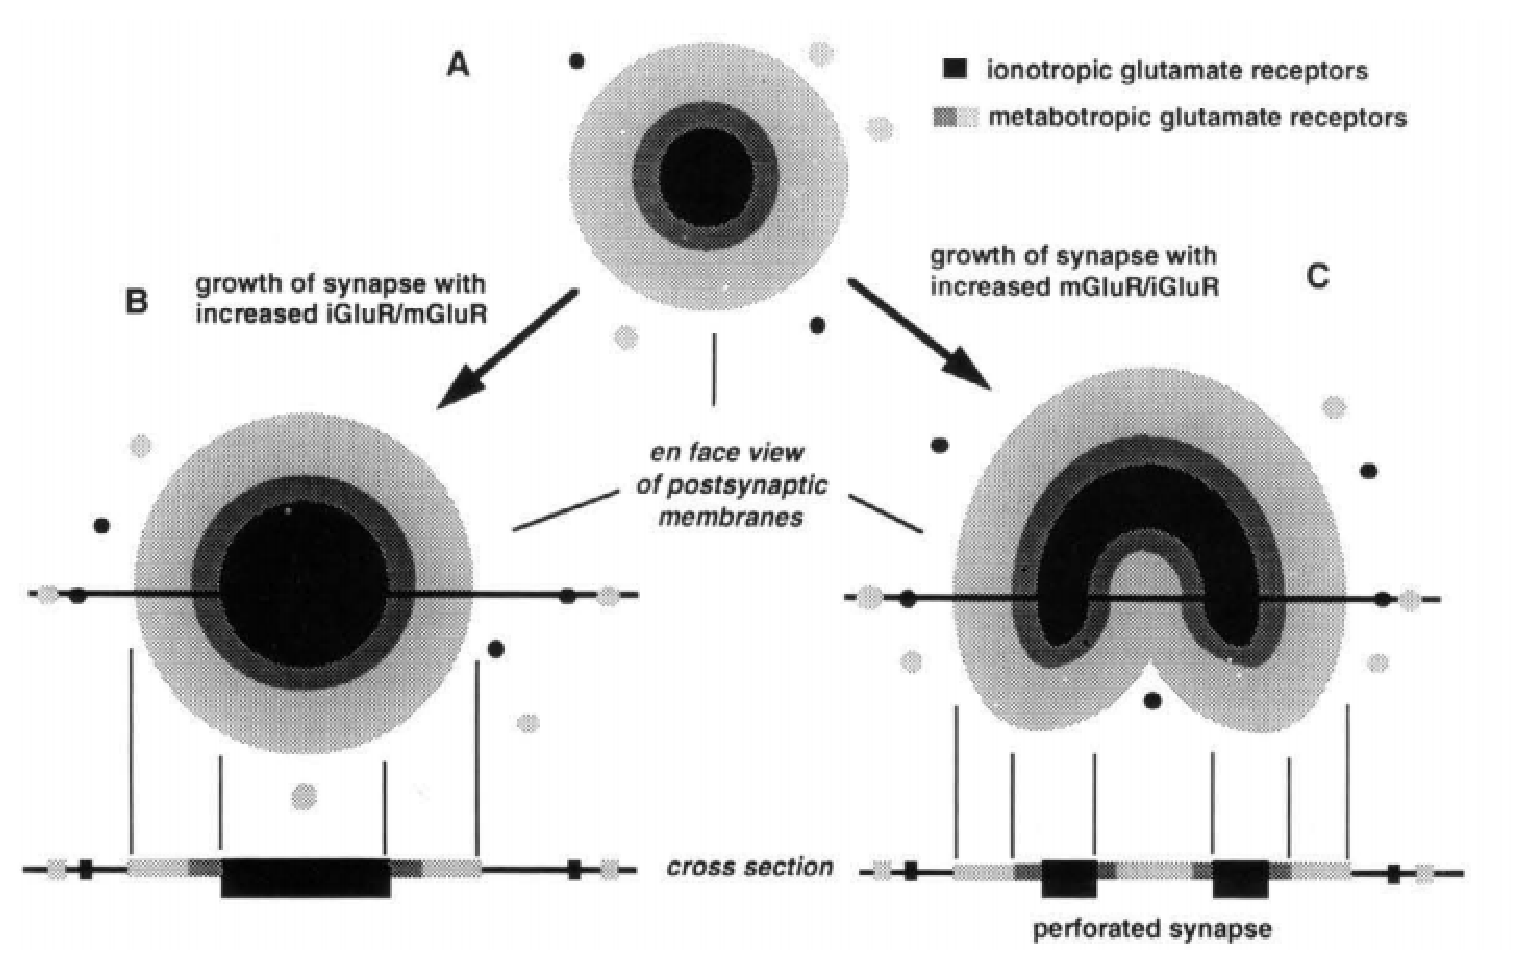
\includegraphics[height=7cm,
    angle=0]{./images/GluR-distribution-synapse.eps}}
  \caption{Schematic summary of glutamate receptors distribution on the
  postsynapse: black = iGluR, stippled = mGluR: (A) inner most is iGluR; then
  mGluR1 + mGluR5, followed by a wider band of receptors decreasing in density.
  Both classes (iGluR, mGluR) occur at a lower density further in the
  extrasynaptic membranes. (B) When synapse grows in size with the regular
  shape: the ratio iGluR/mGluR increases; (C) When synapse grows in size with an
  irregular shape: the ratio iGluR/mGluR decreases }
  \label{fig:GluR-distribution-synapse}
\end{figure}

\section{Transmitter-gated ion channels}
\label{sec:transmitter-gated-ion-channel}

The superfamily of transmitter-gated ion channels 
includes the nicotinic acetylcholine, strychnine-sensitive glycine and 5HT3
receptors. 

They are structurally very similar, composed of five subunits that arrange
together to form an ion channel.

\section{*3. Glycine receptor}
\label{sec:Glycine-receptor}


is an important class of synaptic ion channels ({\it nocotinic
superfamily}) which comprises ACh (Sect.\ref{sec:acetylcholine_receptor}), GABA
(A and C - Sect.\ref{sec:GABAA-receptor}, Sect.\ref{sec:GABAC-receptor}), and
5-HT3 receptors (Sect.\ref{sec:5-HT3-receptor}).

GlyR mediates fast synaptic transmission. It's pentameric, i.e.
$\alpha 1-\alpha 4$ and $\beta$ subunits, arranged in quasi-symmetrically in
circular order around the channel pore which is selective to chlorine.
In mammalian, adult form of GlyR has three $\alpha_1$ subunuits and two $\beta$
subunits. 

Binding the ligand in the extracellular domain produces a series conformational
changes that lead to the opening of the channel. It has three agonist binding
sites (two between $\alpha_1$ and $\beta$ subunits, and one between two
$\alpha_1$ subunits).

Glycine receptor is the receptor activated upon binding of Glycine
(Sect.\ref{sec:Glycine}) 
\begin{itemize}
  \item GLRA1 gene encode $\alpha_1 $ subunit 
  
Mutations lead to the production of a flawed receptor that is unable to respond
properly to glycine.

  \item GLRB gene encode $\beta$ subunit
  
\end{itemize}

The heteromeric $\alpha_1\beta$ form is the most widely studied whose kinetics
was modelled using GABA receptor model, one with cooperativity, and one with
no-cooperativity, Fig.\ref{fig:GlyR_model} \citep{jones1995, burzomato2004}.
Sect.\ref{sec:GlyR_example} describes the modeling of GlyR gating.
$A_x$ indicates $x$ agonist molecules are bound. The second scheme has less
free parameter (14 instead of 18) to estimate. Also even though without the
cooperativity effect, the increase in open efficacy is there and is explained by
the presence of 'flip states' $A_xF$.

\begin{figure}[hbt]
  \centerline{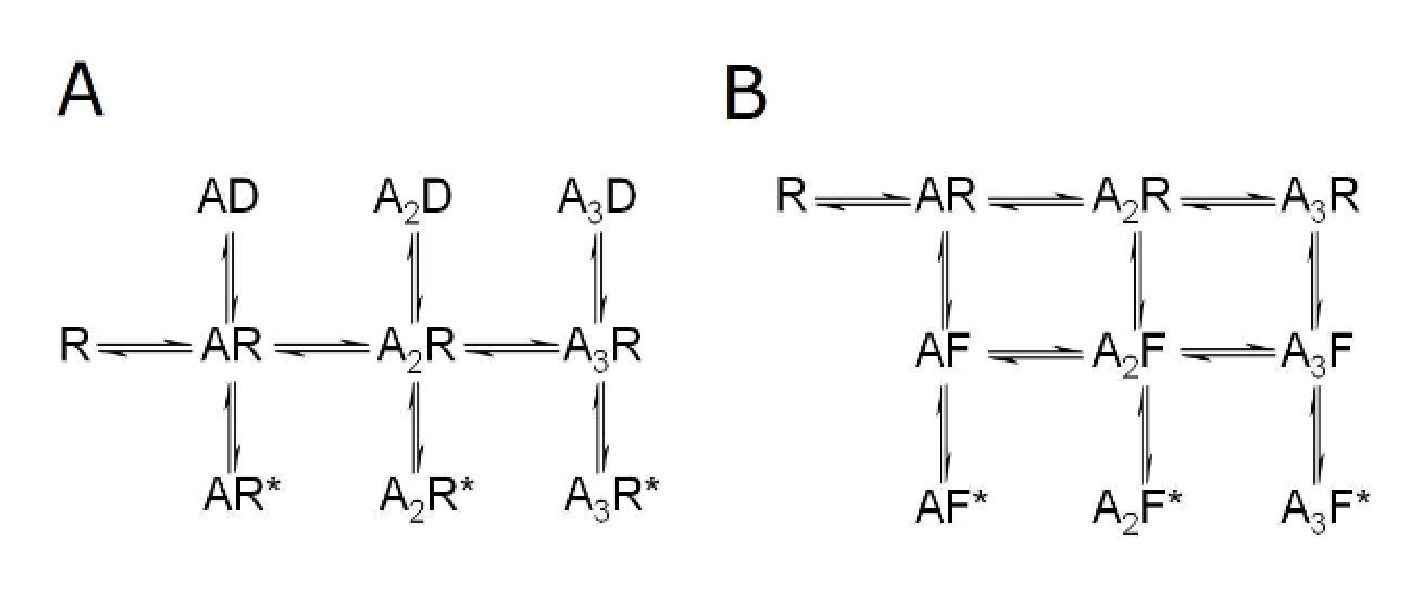
\includegraphics[height=5cm,
    angle=0]{./images/GlyR_model.eps}}
  \caption{Heteromeric $\alpha_1\beta$ GlyR: (A) Model with cooperativity, (B)
  Flip model (no cooperativity). The superscript * marks open states}
\label{fig:GlyR_model}
\end{figure}

The homoeric $\alpha_1$ form like glycine $\alpha_1$ receptor was postulated to
have either 3 or 5 binding sites. The two cases cannot be distinguished, so it's
hypothesized that the gating reactions saturates after three agonists bound.
For the homomeric $\alpha_2$ form, it was modeled with two binding sites
\citep{mangin2003} (Fig.\ref{fig:GlyR_alpha2_model}), and then three
\citep{wang2007}.

\begin{figure}[hbt]
  \centerline{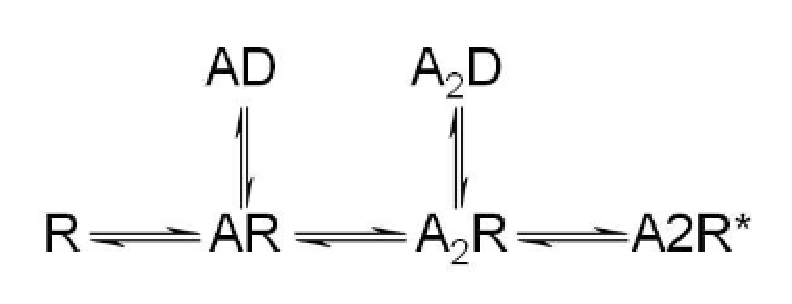
\includegraphics[height=2cm,
    angle=0]{./images/GlyR_alpha2_scheme2bindingsite.eps},
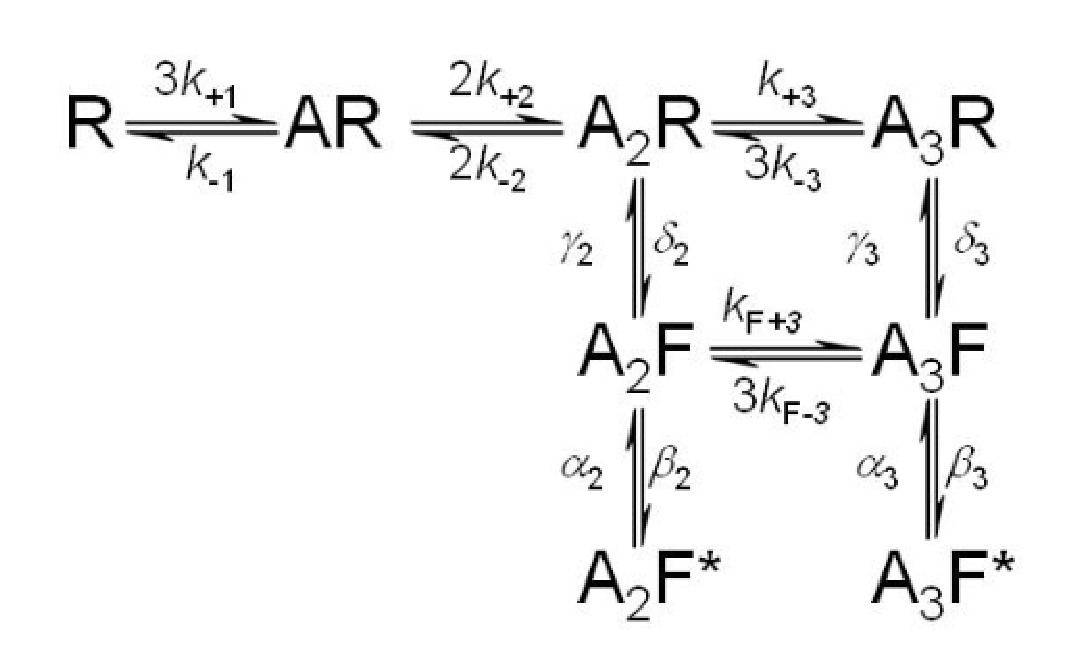
\includegraphics[height=3cm,
    angle=0]{./images/GlyR_model_2.eps}}
  \caption{(A) $\alpha_2$ GlyR scheme with 2 binding sites; (B) Heteromeric
  $\alpha_1\beta$ GlyR scheme that need to be estimated}
\label{fig:GlyR_alpha2_model}
\end{figure}



\section{*3.1. Acetylcholine receptor (AChR)}
\label{sec:acetylcholine_receptor}
\label{sec:cholinergic-receptor}

Cholinergic receptors (acetylcholine receptors, AChR) are integral membrane
proteins that respond to the binding of neurotransmitter acetylcholine as
the agonist (Sect.\ref{sec:Acetylcholine}).

There are two types of AChR:
\begin{itemize}
  
  \item nicotinic receptor (nAChR) (ionotropic acetylcholine receptors):
  ligand-gated (responsive to  nicotine), and is ion-permeated ion channel -
  Sect.\ref{sec:nAChR}
  
  
  \item muscarinic receptor (mAChR) (metabotropic acetylcholine receptors) -
  Sect.\ref{sec:mAchR}):  response to muscarine (a natural product found in
  certain muschrooms)
  
  It is a type of G  protein-coupled receptor.
\end{itemize}


Under the assumption of diffusion-limited reaction
(Sect.\ref{sec:diffusion-limited-reaction}), \citep{land1981} showed that:
diffusion constant for Acetylcholine $D=400\mum^2/sec$ (slightly slower than
free diffusion, which was later estimated to be 280 \citep{madsen1987}), forward
binding rate $k_\on = 4.7\times 10^7 (1/(M.sec))$ (which was later revised to
$3.3\times 10^7$ by \citep{land1984} and then $7.6\times 10^8 (1/(M.sec))$
\citep{madsen1987}), channel relaxation rate $k_\off = 25000$ (1/sec); channel
opening rate constant 8100 sec$^{-1}$, equilibrium dissociation constant $K_d=58
\muM$
\citep{madsen1987}

\subsection{AChR count}
\label{sec:AChR-count-per-synapse}

nicotinic acetylcholine receptors in 
\begin{enumerate}
  \item  neuromuscular junction 
  
  Fertuck and Salpeter (1974) estimated > 8000 receptors/$\mum^2$.
\end{enumerate}


\subsection{AchR (presynaptic)}
\label{sec:acetylcholine-receptor-presynaptic}
\label{sec:cholinergic-receptor-presynaptic}



\section{-- Nicotinic AChR (nAChR)}
\label{sec:nAChR}

% [NOTE: {\it ACh is the neurotransmitter and natural agonist of nAChR; {\it
% nicotine} is another agonist to the receptor which gives the receptor type its
% name, nAChR}]. 

Nicotinic AcetylCholine Receptor (nAChR) is a subfamily of acetylcholine
receptor (Sect.\ref{sec:acetylcholine_receptor}) which is very important in
studying nerve cells. nAChR has 2 types:
\begin{enumerate}
  \item Nm: located in the skeletal cell at the neuromuscular junction
  (Sect.\ref{sec:neuromuscular-junction})
  
  \item Nn: located in the basal ganglia, which upon ligand binding, opening of
  Nn causes the depolarization  in autonomic ganglia resulting in post
  ganglionic impulse.
\end{enumerate}
This channel is non-selective and permeate both $\Na$
and $\K$, with some subunits combination (i.e. the Nn subtype) also permeate
$\Ca$.

\subsection{structure}

Its 0.9nm resolution structure was determined using cryo-electron microscopy,
which shows 5 integral membrane subunits (symmetrically arranged around a
central pore of diameter 0.65nm when opening) in a stoichiometry:
a$_2$bgd, with 
\begin{itemize}
  \item a (alpha subunit) = 437 amino acids, 
  \item b (beta subunit) = 469 (a.a), 
  \item g = 489 (a.a.), 
  \item d (delta subunit) = 501 (a.a.). 
\end{itemize}
Each subunit has 4 TM domains: M1, M2, M3 and M4.

nAChR complex has two binding sites for acetylcholine (ACh), each one is at the
N termini of each alpha subunit, Fig.\ref{fig:nAChR}.
The opening of the channel requires the binding of two ACh molecules.
Coupling betwen two ACh molecules and nAChR is an allosteric
mechanism as the binding of a ligand cause a structural change at a distant
place in the receptor unit, i.e.
each binding leads to 15$^\circ$ rotation of all M2 helices.


\begin{figure}[hbt]
  \centerline{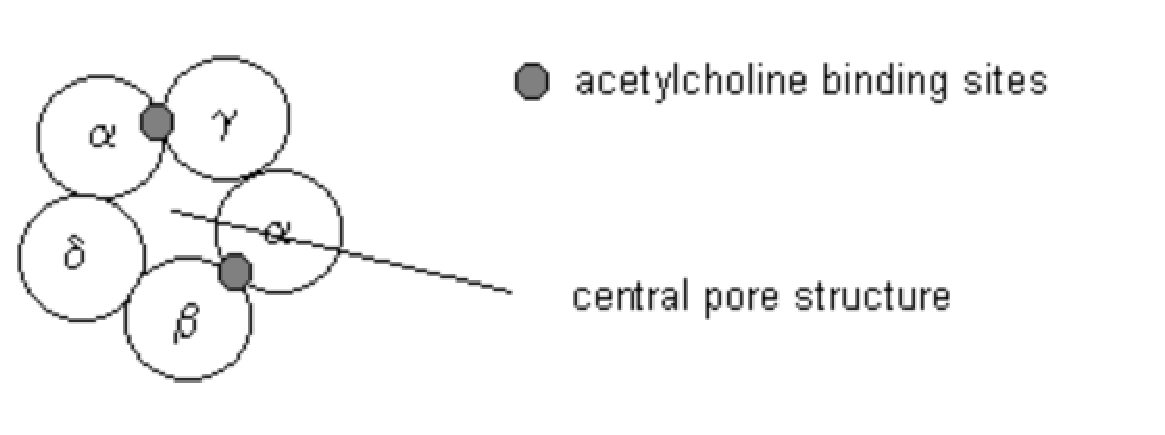
\includegraphics[height=4cm,
    angle=0]{./images/nAChR.eps}}
  \caption{Pentameric arrangement of nAChR subunits}
\label{fig:nAChR}
\end{figure}

In neuron, the binding site of nAChR is located at either the $\alpha$
and (either $\gamma$ or $\delta$) subunits.  
There are 17 nAChR subunits
identified (with $\alpha2-\alpha7$, $\beta2-\beta4$ cloned in humans, the
remaining found only in chicks and rat).

The transmembrane topology of nAChR was inferred from {\bf hydrophobicity
analysis} and {\bf secondary structure predictions} of the primary sequence.
{\bf Hydropathy plots} can tell groups of hydrophobic stretches in the sequence
that are spanning across the membrane, usually in the form of $\alpha$-helix,
Fig.\ref{fig:nAChR_hydropathy_plot}.

\begin{figure}[hbt]
  \centerline{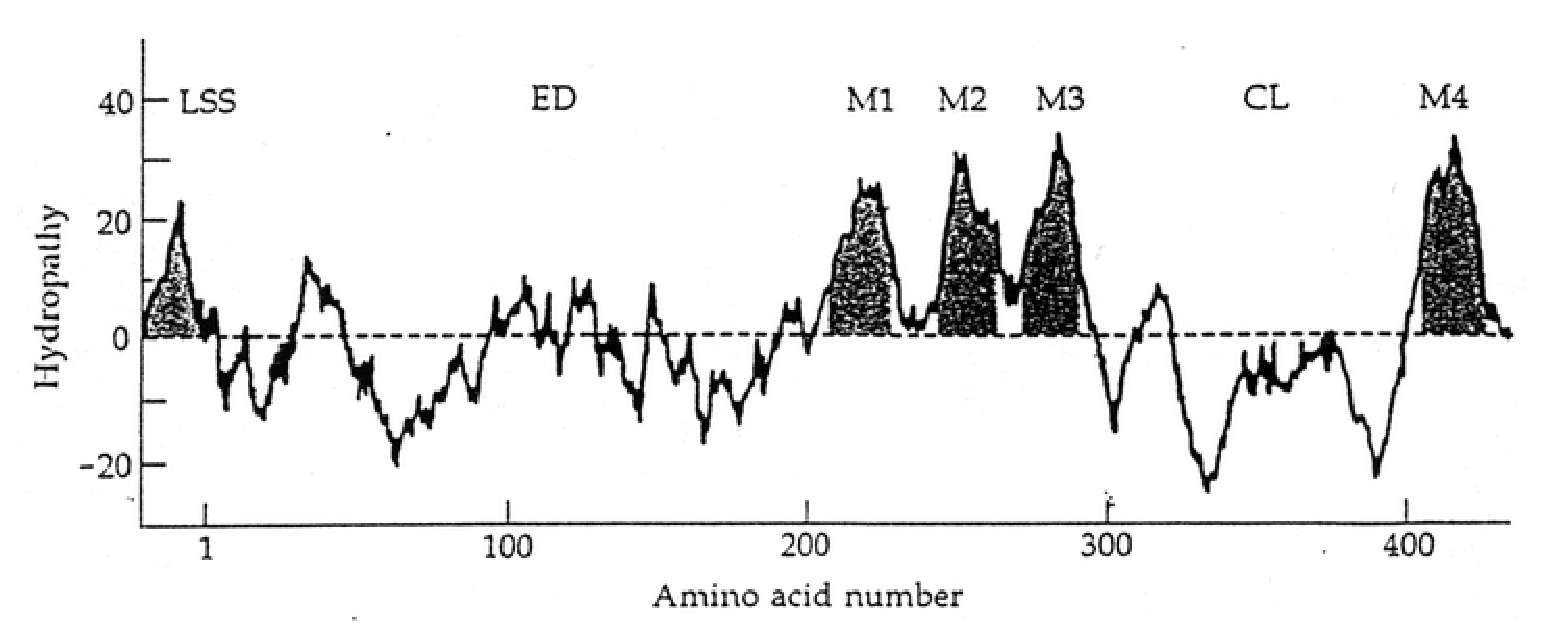
\includegraphics[height=4cm,
    angle=0]{./images/hydropathy_plot_nAChR.eps}}
  \caption{LSS=leader signal sequence, ED=extracellular domain, M1-M4:
  transmembrane spanning domain, CL=cytoplasmic domain}
\label{fig:nAChR_hydropathy_plot}
\end{figure}



\subsection{nAChR: alpha-7 channel ($\alpha$-7)}
\label{sec:alpha-7-nAChR}

Alpha7 ($\alpha7$) nAChR is encoded by CHRNA7 gene in human. The channel is
highly permeable to $\Ca$ and $\Na$, which opens rapidly and tends to remain
open until the agonist diffuses away (usually take 1 ms). The channel is a new
target for drug discovery as the channels have been implicated in
patholophysiology of Alzheimer's disease and schizophrenia (a mental disorder)
\citep{jensen2005, gotti2006}. The positive allosteric modulators (PAMs) of
$\alpha7$ nAChR have been reported to improve cognition and normalize sensory
gating deficits in rodents \citep{timmermann2007, gronlien2007}. 

As a potential drug target, it's important to know all $\alpha7$ nAChR agonists
and PAMs. Upon agonist activation of $\alpha7$ nAChR (tested in GH4-C1
cells\footnote{GH4-C1 cell = a cell line to study electrophysiology on plasma
membrane calcium channels}), the calcium influx through the channel can activate
L-type calcium channels expressed in these cells \citep{feuerbach2005}.


The kinetics of the channel is quite hard to study. Using QPatch Assay Software
(Sophion Bioscience) (which uses either 4 or 8 pipette tips to apply compounds
to the patch-clamped cells), \citep{friis2009} can performs up to 48 independent
patch-clamp experiments in parallel in a 16- or 48-channel chip array called
QPlate. Typically, 5$\muL$ of ligands added for 2sec followed by washout (using
4x of 5$\muL$ of saline). The compounds flow via integrated microfluidic
pathways (in the QPlate) to the patch-clamped cells where the response is
recorded using the built-in amplifiers. The data can be recorded at 5 kHz for
5sec, with membrane potential held at -90mV. The data are analyzed using QPatch
Assay Software.

\subsection{Agonist/Antagonist}

\begin{itemize}
  \item ACh (acetylcholine): the agonist
  	\begin{enumerate}
     \item The rise time $\tau_{TTP}=$5.7$\pm$0.9 (ms) with peak 200pA in
   response to 10mM ACh. Other curves of [ACh] vs. current is displayed in Fig.2(A) of the
  paper \citep{friis2009}
     \item Using double-pulse protocol where [ACh] was increased twice, the
   ratios of the peaks at different concentration of [ACh] were given in Table 1 of the
  paper \cite{friis2009} 
     \item In a biological system, a small change in ligand concentration
     result in rapidchances in response, i.e. following a sigmoidal
     function. In this curve, EC$_{50}$ is the point at which the response
     begins to slow. The half-maximal effective concentration EC$_{50}$ of [ACh]
     (the most common dose-reponse curve for agonist/stimulator) with area-under-the-curve
     (AUC) was 26$\muM$ (compared to 29$\muM$ measured in conventional patch
     clamp).
    \end{enumerate}
    
  \item Nicotine: partial agonist
  \begin{enumerate}
    \item EC$_{50}$ of nicotine was 2.8$\muM$, 
    \item AUCmax=0.4 compared to ACh, i.e. nicotine is only partial agonist with
    a higher affinity than  ACh but with a lower efficacy. 
  \end{enumerate}
  
  \item PAM: the modulators, i.e. the compounds that modulate $\alpha7$ AChR
  (type I PAM increase peak amplitudes with little or no effect on
  desensitization kinetics; type II PAM change the current kinetics by slow
  desensitization kinetics)
  \citep{gronlien2007}
  \begin{enumerate}
    \item type I PAM: NS1738 with EC$_{50}$=12.5$\pm 1.5\muM$
    \item type II PAM: PNU-120596 with EC$_{50}=4.9\pm 1.1\muM$
  \end{enumerate}
  
  \item methyllycaconitine (MLA) : the inhibitor
  \begin{enumerate}
     \item The half-maximal inhibition concentration IC$_{50}$ of the antagonist
     MLA (the most common dose-reponse curve) is 0.25nM
     (similar to published data). 
  \end{enumerate}
\end{itemize}


\section{-- Muscarinic acetylcholine receptor (mAChR)}
\label{sec:mAchR}
\label{sec:muscarinic-acetylcholine-receptor}

Muscarinic acetylcholine receptors (muscarine cholinergic receptor) are members
of rhodopsin-like G-protein coupled receptor family
(Sect.\ref{sec:rhodopsin-like-GPCR}). 

There are 5 subtypes: M1, M2, M3, M4 and M5; divided into 2 categories:
(Jiang et al., 2014).  Among them, M1R (Sect.\ref{sec:M1-muscarinic-receptor})
is widely expressed in the central nervous system and has been implicated in
many physiological and pathological brain functions.

\begin{enumerate}
  
  \item Gq/11: M1, M3 and M5 preferentially interact with Gq/11 
  (Sect.\ref{sec:Gq/11-protein})
  
  They activate phospholipase C  (Sect.\ref{sec:GPCR-PLC-IP3-DAG-pathway})

  \item Go/i: M2 and M4 subtypes preferentially interact with Go/i

The activation of this receptor deactivates adenylate cyclase and causes a
decrease in cAMP in the cell, generally leading to inhibitory-type effects
(Sect.\ref{sec:cAMP-dependent_pathway}).

The G$_{\beta\gamma}$ subunit activates the K-channels and therefore
hyperpolarize the cell. This causes a decrease in cardiac activity.

\end{enumerate}



\subsection{M1R, M3R}
\label{sec:M1-muscarinic-receptor}
\label{sec:M3-muscarinic-receptor}

M1 mAChR is one member of the Gq/11 GPCR muscarinic receptor
(Sect.\ref{sec:muscarinic-acetylcholine-receptor}) activated by acetylcholine
(Sect.\ref{sec:acetylcholine_receptor}).

M1-R is widely found in central neurvous system and is postulated to be an
important therapeutic target for AD and several other neurodegenerative
diseases.

Activation of M1 mAChR
\begin{itemize}
  \item enhance sAPP$\alpha$ generation and reduce A$\beta$ production
  
  \item activate PKC (Sect.\ref{sec:PKC}) 
  
  \item affects BACE1 (rate-limiting enzyme for A$\beta$ generation in
  Alzheimer's disease)
\end{itemize}

\subsection{M2 receptor (heart + neuron)}
\label{sec:M2-receptor}

M2 muscarinic receptors are located in the heart, where they act to slow the
heart rate down to normal sinus rhythm 
They reduce the speed of depolarization. They also reduce contractile forces of
the atrial cardiac muscle, and reduce conduction velocity of the
atrioventricular node (AV node). However, they have no effect on the contractile
forces of the ventricular muscle.

Compared to M4 receptors, the M2 subtype of acetylcholine receptor functions
similarly as an inhibitory autoreceptor to acetylcholine release, albeit
functioning actively primarily in the hippocampus and cerebral cortex.

\url{https://en.wikipedia.org/wiki/Muscarinic_acetylcholine_receptor_M2}

\subsection{M4 receptor (neuron)}
\label{sec:M4-receptor}

M4 receptor is coupled to to Gi/o heterotrimeric protein
(Sect.\ref{sec:Gi/o-protein}).

Activation of M4 receptors inhibits acetylcholine release in the striatum. 



\section{*3.2. GABA receptors}
\label{sec:GABA_receptors}

GABA (Sect.\ref{sec:GABA}) is the endogeneous ligand to GABA
receptors. 


GABA receptors are receptors that can be on presynaptic side or
postsynaptic sides of neurons. 
\begin{itemize}
  \item Those on the presynaptic side function as autoreceptor
  that regulates the release of GABA neurotransmitter from the same neuron
  (Sect.\ref{sec:GABA-receptor-presynaptic}).
  
  \item  Those on the postsynaptic side receives the signal from GABAergic neurons
(Sect.\ref{sec:GABAergic-neurons}) and trigger chlorine influx (i.e.
hyperpolarizing current).
  
\end{itemize}

The principal inhibitory neurotransmitter GABA (Sect.\ref{sec:GABA}) exerts its
effect on
\begin{enumerate}
  \item two ligand-gated ion channels ($\Cl$-permeable (moving in) or $\K$
  (moving out)):   GABA$_A$, and GABA$_C$ - Sect.\ref{sec:GABAA-receptor-GABAC-receptor}
   
  
They belong to the family of transmitter-gated ionic channels
(Sect.\ref{sec:transmitter-gated-ion-channel}),
and are fast-acting {\bf ionotropic receptors}.
 
  \item one class-C GPCR called GABA$_B$: Sect.\ref{sec:GABAB-receptor}
  
  
slower (metabotrophic) GABA$_B$ ({\bf metabotropic receptors}) with 7 TMS
(Sect.\ref{sec:GPCR}), i.e. the binding of GABA link to and control ionic
channels via a signal transduction, mainly G-proteins.
   
\end{enumerate}

GABA receptors, Fig.\ref{fig:GABA_receptor}, are pentamers most commonly
composed of three different subunits ($\alpha, \beta, \gamma$), though several
other subunits ($\delta, \epsilon$, $\theta, \pi, \sigma$) and conformations
exist.

\subsection{GABAR number}
\label{sec:GABAR-count}

The number of GABAR per synapses (see also Masugi-Tokita et al., 2007)
\begin{enumerate}
  \item cerebellar stellate cells
  
  Nusser et al. (1997) estimated 1250 receptors/$\mum^2$.
  
\end{enumerate}

\subsection{GABA-A and GABA-C receptors}
\label{sec:GABAA-receptor-GABAC-receptor}

Depending on the types of receptors, the open channels are selectively permeable
to either chloride (moving in) or potassium ions (going out). IMPORTANT: GABA is
an order of magnitude less potent at GABA-A  than GABA-C receptors.

Recently, different associated proteins have been cloned that link these
receptors to the cytoskeleton
\begin{enumerate}
  \item GABA-A receptor links to cytoskeleton via $\gamma$2-subunit by 
  GABA-A-receptor-associated proteins (GABARAP).
  
  \item GABA-C receptor links to cytoskeleton via $\rho$1-subunit by 
  microtubuleassociated protein 1B (MAP-1B).
\end{enumerate}
The fact that two different proteins associate with the GABAA
and GABAC receptors allows these receptors to
exist and function separately.



\subsection{-- GABA-A receptor}
\label{sec:GABAA-receptor}


GABA-A receptors is one of the two
GABA-gated ion channels (Sect.\ref{sec:GABAA-receptor-GABAC-receptor}). 

In human, there are 16 subunits that can comprise a single GABA-A receptor:
\begin{enumerate}
  \item $\alpha$1-16
  
  \item $\beta$1-4
  
  \item $\gamma$1-4
  
  \item $\delta$
  
  \item $\varepsilon$
\end{enumerate}

A GABA-A receptor is a hetero-oligomeric structure of mixed subunits.
However, a fully functional receptor, GABA-A needs to have at least an $\alpha$,
$\beta$ and one other subunit type.

GABA-A is the receptors responsible for the major GABAergic inhibitory
in adult CNS.  GABA-A produces 2 forms of inhibition: {\bf phasic} (synaptic)
and {\bf tonic} (extrasynaptic) forms of inhibition 

\begin{enumerate}
  
  \item {\bf phasic mode}: postsynaptic active region with rapid increase in
  [GABA] (0.3 - 1 mM) due to presynaptic vesicle release, and GABA binding cause
  GABA-A opening. This happens in a very short time (< 1 ms) due to reuptake and
  fast diffusion of GABA, and induces {\bf IPSC} (Sect.\ref{sec:IPSC})
  
Phasic inhibition is essential in setting the temporal window for synaptic
integration (Farrant \& Nusser, 2005), and may also generate rhythmic network
activities (Cobb et al, 1995; Huntsman et al, 1999)
  
  \item {\bf tonic mode}: is the slower form of inhibition. With high [GABA] in
  the extracellular space (extrasynaptic), they binds to high-affinity
  extrasynaptic and perisynaptic GABA-A receptors. This induces {\bf tonic
  current}.
  
 As GABA-A locates outside the postsynaptic active, GABA-A play a role in the
 tonic inhibition.  Although tonic current is small in amplitude, the
persistent inhibition is likely central for modulating cellular excitability.

\end{enumerate}
\textcolor{red}{It has been proposed that tonic inhibition plays a critical part
in controlling neuronal and network excitability}.
Tonic GABA(A) receptor-mediated currents were present in pyramidal cells and
interneurons in layer V-VI of temporal neocortex and granule cells in the
dentate gyrus (Sect.\ref{sec:dentate_gyrus}). These tonic currents have cell
type-specific pharmacologies, opening up the possibility of targeted therapeutics.


Under binding two agonist GABA molecules, GABA$_A$ opens and allows $\Cl$, and
to a lesser extent $\ce{HCO3^-}$ inflow.
Because chloride ions are negatively charged, this hyperpolarizes the cell
membrane and brings it further away from firing an action potential.
The hyperpolarization of postsynaptic potential results in reduced neuronal
activity. 

\textcolor{red}{Agonists}: In GABA-A receptor, these are activators: GABA,
TACA, and CACA. Also, the compounds muscimol and its conformationally restricted
analogue THIP (Sect.\ref{sec:Muscimol}), act at both GABAA
and GABAC receptors. Muscimol is agonist to GABA-A receptor; while THIP is only
a partial agonist.

\textcolor{red}{Antagonist}: GABAA receptors are selectively blocked by the
alkaloid bicuculine and are modulated by benzodiazepines, steroids and
barbiturates.

\textcolor{red}{conductances}: Single channel electrophysiological studies using
outside-out patches from rat retinal bipolar cells showed that GABAC receptors
conducted less current than GABAA receptors.

\subsection{GABA-C receptor}
\label{sec:GABAC-receptor}

There are two human GABA-C receptor subunits
\begin{enumerate}
  \item  $\rho$1 and $\rho$2.

IMPORTANT: The $\rho$ subunits do not assemble with $\alpha$ and $\beta$
subunits to form a receptor

\end{enumerate}
with the receptor is a homo-oligomeric structure made of either one of the two
above; though there are evidences that these receptors may be hetero-oligomeric.


IMPORTANT:
\begin{enumerate}
  \item  GABA-C is also a chlorine-sensitive channels, yet with a much stronger
  GABA affinity than GABA-A.

  \item Unlike GABA-A receptor, GABAC receptors are not blocked by bicuculine, nor are
they modulated by benzodiazepines, steroids or barbiturates.
\end{enumerate}

% NOTE: In GABA-A receptor, these are activators: GABA, TACA, and CACA.
% Bicuculine can block the effect of GABA and TACA; but not CACA.

\textcolor{red}{\bf Agonists}: Also, the compounds muscimol and its
conformationally restricted analogue 4,5,6,7-tetrahydroisoxazolo[5,4-c]pyridin-3-ol, act at both
GABAA and GABAC receptors.
THIP is agonist to GABA-C receptor; while moscimol is only a partial agonist.
This is in opposite to GABA-A receptor; and thus  THIP can be
used to pharmacologically distinguish these receptors.


\textcolor{red}{\bf Antagonist}: 
GABA-C receptor is insensitive to both bicuculine and baclofen.
Instead, GABAC receptors are activated by CACA -
Z-4-aminobut-2-enoic acid (cis-aminocrotonic acid (CACA))3,4 and 
(1S,2R)-(+)-2-(aminomethyl)-cyclopropane-1-carboxylic acid ((1S,2R)-(+)-CAMP; 
[RK Duke et al., unpubl. obs., 1998], and are selectively blocked
by (1,2,5,6-tetrahydropyridin-4-yl)methylphosphinic acid (TPMPA).


\textcolor{red}{conductances}: Single channel electrophysiological studies using
outside-out patches from rat retinal bipolar cells showed that GABAC receptors
conducted less current than GABAA receptors. 
\begin{itemize}

  \item  When activated, GABAC receptors had a longer
channel opening time and desensitized less readily with maintained agonist
application.

  
\end{itemize}

\subsection{GABA-B receptor}
\label{sec:GABAB-receptor}


GABA-B receptor is a class-C GPCR (Sect.\ref{sec:GPCR}) that 
upon activation, activate the second messenger systems phospholipase C and
adenylate cyclase to regulate potassium ($\K$) and calcium ($\Ca$) channels.
\begin{enumerate}
  \item GIRK - Sect.\ref{sec:GIRK}
\end{enumerate}

There are two locations of GABA-B
\begin{itemize}
  \item presynaptic GABA-B: functions as autoreceptors and mediate a reduction
  in $\Ca$ current at the nerve terminal

As a GPCR, pre-synaptic GABAB  receptors produce slow, prolonged inhibitory
signals and function to modulate the release of neurotransmitters. 
  
  \item postsynaptic GABA-B: activates $\K$ channales and hyperpolarize the
  neurons
\end{itemize}


There are 3 subunit types found in GABA-B receptors
\begin{enumerate}
  \item GABA-B1a
  
  \item GABA-B1b
  
  \item GABA-B2
\end{enumerate}

The first GABA$_B$ receptor cDNAs were isolated only in 1997 (Kaupmann et al.,
1997).  The identification of a second GABA$_B$ receptor protein soon after led
to the discovery that native GABAB receptors are heterodimers composed of two
subunits, GABA-B1 and GABA-B2  (reviewed in Calver et al., 2002; Bettler et al.,
2004).   GABA-B receptors expressed with only GABA-B1 (GABA$_B$R1) even though
still show high-affinity antagonist-binding sites; they produce little of the functional
activity expected from studies of endogenous GABAB receptors in the brain
\citep{jones1998}.

A fully functional GABAB receptors are  hetero-oligomeric formed either
(GABA-B1a or GABA-B1b) forms with GABA-B2 subunit, i.e. confirmed when these
subunits are expressed in Xenopus oocytes or mammalian cell expression systems.
Double immunoprecipitation studies have shown that these subunit combinations
also exist in vivo as either dimers or multimers.
\begin{enumerate}
  \item  Neither GABA-BR1 or GABA-BR2 can activate GIRK-type potassium
  channels (Sect.\ref{sec:GIRK})
  
  \item The   combination of GABABR1 and GABABR2 confers robust stimulation of
  channel activity
  
  
\end{enumerate}

In the brain two predominant, differentially expressed splice variants
are GABA-B1a, and GABA-B1b. The a functional role of GABA-B1c has yet to be
determined, although it may play a role in the developing human brain.

\textcolor{red}{Agonists}:  (R)-(-)-baclofen and the phosphinic acid analogue of
GABA (3- aminopropyl)phosphinic acid (CGP27492).

\textcolor{red}{Antagonists}: phaclofen and saclofen, respectively, selectively
antagonize these receptors.



\subsection{Binding mechanism}

At rest, the neuron membrane potential is about -65 mV. The resting potential
for chlorine channels is about -70mV, and the concentration of chlorine is much
higher outside (Sect.\ref{sec:ion-concentration-neuron}).
When GABA bind to chlorine channels in the plasma membrane of both pre- and
postsynaptic neuronal process, the ion channels open to allow more ion chlorine
into the cell and charged potassium ions out of the cell. This causes a
hyperpolarization, i.e. inhibitory process.

\begin{itemize}
  \item GABA is synthesized from glutamate from enzyme GAD67 (Glutamate
  decarboxylase)
  \item GABA is transported in vesicles to the presynaptic terminal.
  \item GABA activates the chlorine channels in the presynaptic terminal.
\end{itemize}

\begin{figure}[hbt]
  \centerline{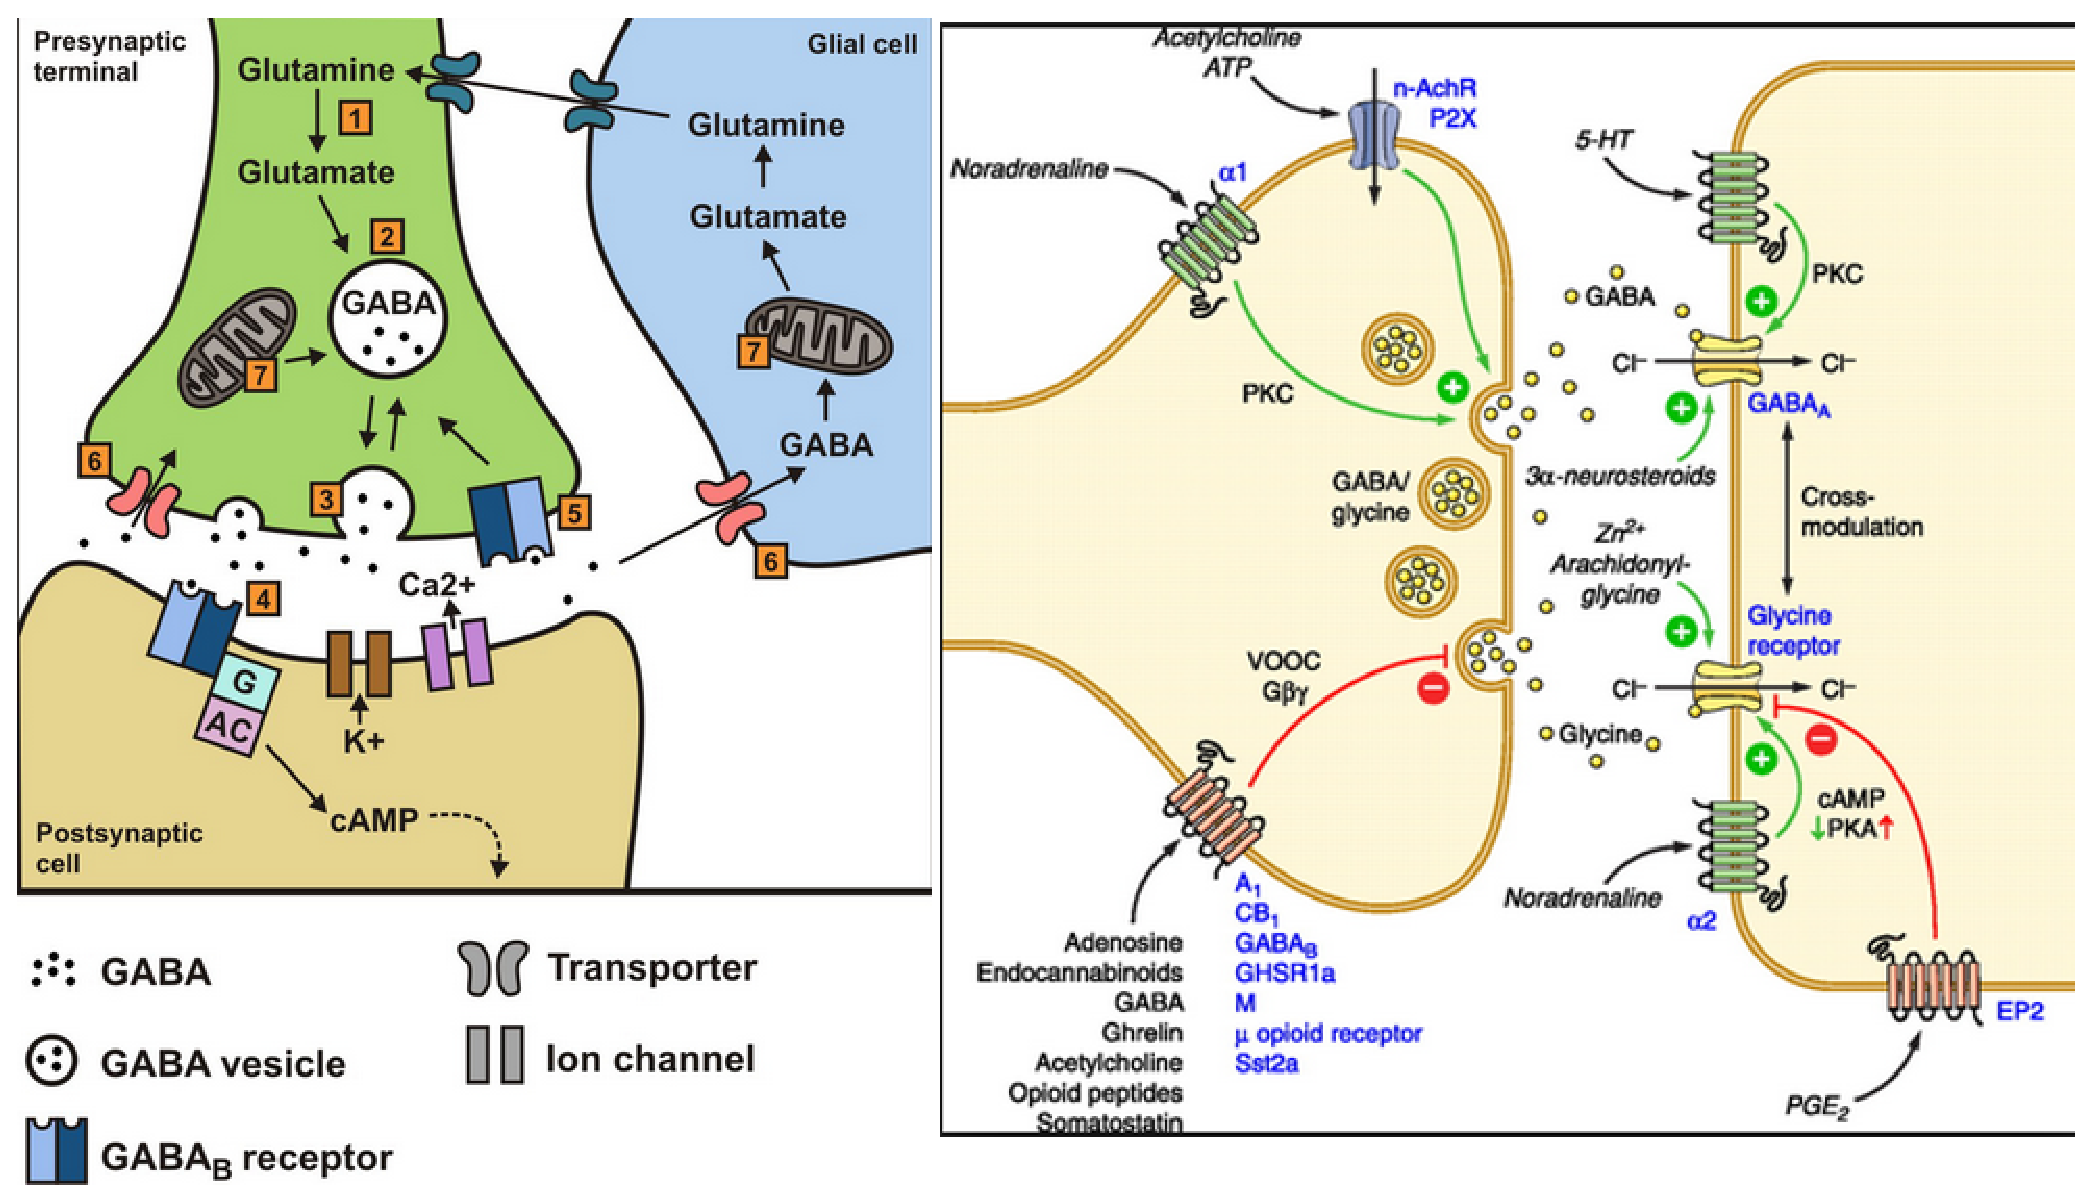
\includegraphics[height=6cm,
    angle=0]{./images/GABA_receptors.eps}}
  \caption{GABA receptors: GABA$_B$ and $GABA_A$}
  \label{fig:GABA_receptor}
\end{figure}

\subsection{GABA receptor (presynaptic)}
\label{sec:GABA-receptor-presynaptic}

The channel on the presynaptic side function as autoreceptor, i.e.
regulate the release the GABA neurotransmitter, a character that is also found
in other types of receptors such as aminergic receptors
(Sect.\ref{sec:aminergic-receptors}) and cholinergic receptors
(Sect.\ref{sec:cholinergic-receptor-presynaptic})
  



\section{*3.3. 5-HT3 receptor}
\label{sec:5-HT3-receptor}

5-HT$_3$ receptor is a ligand-gated ion channels ($\Na$ and $\K$), i.e.
once open help depolarize the $V_m$ on postsynaptic side; though other members
of 5-HT receptor family are G-protein coupled receptor
(Sect.\ref{sec:5-HT_receptor}).
  
Preclinical studies suggest that 5-HT3 antagonists may enhance memory and be of
benefit in the treatment of anxiety, depression, pain, and dementia.
  

\section{IP3 receptors}

Check Sect.\ref{sec:IP3R_neuron}. 


\section{Integrins}
\label{sec:integrins}

Integrins are transmembrane receptors that are the bridges for cell-cell and
cell-extracellular matrix (ECM) interactions.
Integrins work alongside other receptors such as cadherins, the immunoglobulin
superfamily cell adhesion molecules, selectins and syndecans to mediate
cell-cell and cell-matrix interaction.

There are several types of integrins, and a cell may have several types on its
surface. 

Ligands for integrins include fibronectin, vitronectin, collagen, and laminin.

\section{Autoreceptors}
\label{sec:autoreceptors}

An autoreceptor is a type of receptor located in the membranes of presynaptic
nerve cells, providing a negative feedback loop in signal transduction.
It is only sensitive to the neurotransmitters or hormones released by the
neuron on which the autoreceptor sits. 

\textcolor{red}{Autoreceptors may be located in any part of the cell membrane:
in the dendrites, the cell body, the axon, or the axon terminals}.
Autoreceptors are usually G protein-coupled receptors (rather than
transmitter-gated ion channels) and act via a second messenger.

\begin{enumerate}
  \item adrenoreceptor = Sect.\ref{sec:adrenoreceptor}
\end{enumerate}

\subsection{Adrenoreceptor: alpha-2A, alpha-2C}
\label{sec:adrenoreceptor}

Only $\alpha-2$ adrenergic receptors inhibition effects
(Sect.\ref{sec:adrenergic_receptor}), so $\alpha-2A$  and $\alpha-2C$
adrenoreceptor on the presynaptic side can inhibit further release of
norepinephrine.

\subsection{D2-like autoreceptor}
\label{sec:D2-like-autoreceptor}


\section{Glycine transporter (GLYT)}
\label{sec:glycine-transporter}

The  concentration  of  glycine  (Sect.\ref{sec:Glycine}) at  synapses  is
mainly controlled by two sodium    and    chloride    dependent transporters,
GLYT1 and GLYT2, proteins   that   display   a   complementary   distribution
and  activity  in the  nervous  system.

\subsection{GLYT1}
\label{sec:GLYT1}

Despite the presence of GLYT1 mRNA in both glial cells and in glutamatergic
neurons, previous studies have mainly localized GLYT1 immunoreactivity to glial
cells in the caudal regions of the nervous system.

\subsection{GLYT2}
\label{sec:GLYT2}


\section{Glutamate transporter}
\label{sec:glutamate-transporter}

Glutamate is the major excitatory neurotransmitter in the mammalian CNS
(Sect.\ref{sec:Glutamate}). The spatiotemporal profile of the glutamate
concentration in the synapse is critical for excitatory synaptic signalling.
The control of this spatiotemporal concentration profile requires the presence
of large numbers of synaptically localized glutamate transporters that remove
pre-synaptically released glutamate by uptake into neurons and adjacent glia
cells.

There are two types of glutamate transporters: 
\begin{itemize}

  \item $\Na$-depenent: (sodium and potassium coupled glutamate transporters)
  EAAT (Sect.\ref{sec:EAAT}). 
  
    
  \item $\Na$-independent: VGLUT (vesicular glutamate transporters) and xCT
  (cystine-glutamate transporter)

  \begin{itemize}
    \item xCT: localized to plasma membrane of cells
    
    \item VGLUT (Sect.\ref{sec:VGLUT}): found on membrane of
    glutamate-containing synaptic vesicles
  \end{itemize}

\end{itemize}

These glutamate transporters are electrogenic and utilize energy stored in the
transmembrane potential and the Na+/K+-ion concentration gradients to accumulate
glutamate in the cell.

Review: Grewer, Rauen (2005)


\subsection{EAAT ($\K+$/$\Na$-dependent)}
\label{sec:EAAT}
\label{sec:GLT1}
\label{sec:EAAC1}
\label{sec:GLAST1}

Excitatory amino acid transporters 1-3 (EAAT1-3) - resides on endothelial cells
(Sect.\ref{sec:endothelial-cell}) - moves glutamate out of the brain against the
large opposing concentration gradient ($< 1 \muM$ in the ISF compared with
$\approx 100 \muM$ in the plasma (blood capillaries)).
These proteins bind to glutamate, one molecule at a time, and transfer them into
the cell.  

EAAT1-2 on astrocytes recycle glutamate out of the synaptic cleft, and then
converted into glutamine inside astrocyte
(Sect.\ref{sec:glutamate-glutamine-cycle}). The transport is Na+-dependent and
accompanied by net uptake of ions and water, again contributing to water
clearance at the blood-brain barrier.u

\begin{mdframed}
EAATs exhibit stereoselectivity for L-glutamate but transport both L- and
D-aspartate.

The first three eukaryotic glutamate transporters: GLAST1 (Glutamate Aspartate
Tansporter 1, (Storck et al., 1992) and GLT1 (Glutamate Transporter 1, (Pines et
al., 1992) from rat brain, and EAAC1 (Excitatory Amino Acid Carrier 1, (Kanai \&
Hediger, 1992) from rabbit small intestine, were almost discovered around the
same time. This led to the standardized nomenclature using the acronym EAAT
({\bf Excitatory Amino Acid Transporter}).
\end{mdframed}


Nowadays, there are 5 known subtypes in human, Fig.\ref{fig:Glutamate_uptake}.
Besides the two new human high affinity glutamate transporters (EAAT4, EAAT5),
there are also two neutral amino acid transporters (ASCT1 und ASCT2 (Alanine
Serine Cysteine Transporter 1 and 2))
%NOTE: In rodents, EAAT1 = GLAST, EAAT2 = GLT1, EAAT3 = EAAC1.

\begin{itemize}
    \item EAAT1, EAAT2 (i.e. EAAT1/2): found on membrane of glial cells
    (astrocytes, microglia, oligodendrocytes)
    
\begin{enumerate}

  \item EAAT1 transporter (in human, encoded by slc1a3 protein) or GLAST1 (in
  rat):   selectively expressed in astrocytes in brain (highest level found in
  cerebellum, and then to forebrain).
  
{\bf SLC1A3} (Solute carrier family 1 (glial high-affinity glutamate
transporter), member 3) is a protein in humans, encoded by {\it SLC1A3} gene.
Other names: GLutamate ASpartate Transporter (GLAST) or Excitatory Amino Acid
Transporter 1 (EAAT1) .
  
  \item EAAT2 (in human, encoded by slc1a2 protein) or \textcolor{red}{GLT1} (in
  rat): GLT1a and GLT1b
  
  EAAT2/GLT1a (predominantly expressed in astrocytes; yet with a smaller amount
  10\% found in axon terminal of CA1 hippocampus (but not found in dendrite)).
  The splice variant GLT1b not found in the neuron after all, but found in
  astrocytes
  
  EAAT2/GLT1 is the most important subtype in the mature brain; which
  \textcolor{red}{represents only 1\% but accounts for about 95\% of total
  glutamate uptake activity for the forebrain}. It has high affinity for
  Glutamate ($\sim 12 \muM$).
  
  Low level of EAAT2 is also found in axon-terminal of CA3 pyramidal cells
  
\end{enumerate}    

\textcolor{red}{To compensate for the slow uptake rate (14 ions/sec)}, the
density of EAAT2 on astrocytes in extraordinarily high (1000-10,000
transporters/$\mum^2$, to be sufficient to capture all released Glu from
terminal).

The loss of EAAT2 expression or function is implicated in different neurological
diseases (e.g. strokes, trauma, MS, ALS, PD, HD, and glioma). The drug {\it
ceftriaxone}, an antibiotics that enhances transcriptional regulator of EAAT2
that can enhance EAAT2 in astrocytes 3-fold is considered a promise candidate
for ALS treatment. 

    \item EAAT3 (in human) or EAAC1 (in rat/rodent): exclusively neuronal
    terminal (expressed in neuronal terminal, cell bodies, and dendrites), yet
    hard to detect as the expression level is quite low (100x lower than those
    of GLT1).


   \item EAAT4 (i.e. EAAT3/4): exclusively neuronal terminal
    (expressed in neuronal terminal, cell bodies, and dendrites), with 
    mostly in cerebellar Purkinje cells (and then in forebrain) 
   
    \item EAAT5: found in retina (Arriza et al., 1997; Fairman et al., 1995)
\end{itemize}


\textcolor{red}{\bf IMPORTANT}: The 5 types of GLUT-transporters share no
significant homology with the family of sodium- and chloride-dependent
neurotransmitter transporters (such as for GABA -
Sect.\ref{sec:GABA-vesicular-transporter}, glycine -
Sect.\ref{sec:glycine-transporter},
Sect.\ref{sec:glycine-transporter-intracellular}, dopamine -
Sect.\ref{sec:dopamine-transporter}, serotonin -
Sect.\ref{sec:serotonin-transporter}, noradrenalin, proline and taurine), nor do
they exhibit any significant homology with any other known protein family.

\subsection{GLAST}
\label{sec:GLAST}

\subsection{--Kinetics}


\subsection{Vesicular glutamate transporter (VGLUT)}
\label{sec:VGLUT}



\section{Vesicular glycine transporter: VIAAT/VGAT}
\label{sec:VIAAT/VGAT}
\label{sec:glycine-transporter-intracellular}

The presynaptic glycine transporter known as GlyT2 is encoded by SLC6A5 gene
whose  missense, nonsense and frameshift mutations links to startle disease
(Sect.\ref{sec:hyperkplexia}).
This is the first human neurological disorder connected to alterations in a
$\Na$/$\Cl$-dependent transporter for a classical fast neurotransmitter.

This vesicular transporter (VGAT) is shared with GABA (Sect.\ref{sec:GABA}),
some terminals contain vesicles that accumulate simultaneously glycine and GABA,
thereby releasing both these neurotransmitter.

\section{Vesicular GABA transporter: VGAT}
\label{sec:VGAT}
\label{sec:GABA-vesicular-transporter}


Neurotransmitters, including GABA (Sect.\ref{sec:GABA}), are stored in synaptic
vesicles at presynaptic nerve terminals. The vesicular GABA transporter, VGAT,
was first cloned in 1996.

VGAT is highly concentrated in the nerve endings of GABAergic neurons in the
brain and spinal cord but also in glycinergic nerve endings, suggesting that
some terminals contain vesicles that accumulate simultaneously glycine and GABA
(Chaudhry et al., 1998).

Although the great majority of nerve terminals containing GABA or glycine are
immunopositive for VGAT, subpopulations of nerve endings rich in GABA or glycine
appear to lack the protein, suggesting there is another vesicular proteins.

There are evidences suggesting at least 2 distinct pools of GABA vesicles are
present at inhibitory synapses in the rat neocortex (Hablitz et al., 2009).
The authors used FM1-43 fluorescence to directly probe for the existence of
distinct vesicular pool.
These multiple pools may play diverse roles in such processes as long-term
depression and/or potentiating of inhibitory synaptic transmission, homeostatic
plasticity of inhibitory activity, or developmental changes in inhibitory
synaptic transmission.


\section{GABA transporters: GAT1, GAT2, GAT3, and BGT1}
\label{sec:GAT-1}
\label{sec:GAT-2}
\label{sec:GAT-3}
\label{sec:BGT-1}

There are four GABA transporters (GAT-1, GAT-2, GAT-3 and BGT-1).
All these transporters are highly hydrophobic proteins with 12 transmembrane
segments, extracellular glycosylation sites, and intracellular consensus sites
for phosphorylation. 



Each binds GABA with varying affinities: BGT1 $\ll$ GAT1 $\ll$ GAT2 $\ll$ GAT3.
\begin{itemize}

  \item BGT1 has lowest affinity

  \item GAT3 has highest affinity
  
 GAT3 uses sodium (Na+) electrochemical gradients to mediate uptake of GABA from
 the synaptic cleft by surrounding glial cells
  
\end{itemize}

Distributions: expressed throughout the brain, with different levels of
expression in different brain regions.
\begin{enumerate}
  \item  GAT2 (SLC6A13) is predominantly expressed in hepatocytes in the liver
  
  also found in proximal tubules in the kidney as well as in the leptomeninges
  and in some blood vessels in the brain
  
  \item GAT-1 is  a sodium- and chloride-dependent GABA transporter 1 involved
  in the process of GABA reuptake into nerve terminals, thus helping to
  terminate its synaptic activity. 
  
\end{enumerate}

GABA transporters are present in neurons and in astrocytes and their activity is
crucial to regulate the extracellular concentration of GABA under basal
conditions and during ongoing synaptic events.

\section{Serotonin transporter (5-HTT)}
\label{sec:serotonin-transporter}

serotonin transporter (SERT or 5-HTT) is $\na$-dependent serotonin transporter.
It terminates the action of serotonin and recycles serotonin by transporting
serotonin from the synaptic cleft to the presynaptic neuron.

Serotonin-Reuptake transporters are dependent on both the concentration of
$\K$ ion in the cytoplasm and the concentrations of $\Na$ and $\Cl$
ions in the extracellular fluid.
In order to function properly the SERT requires $\Na/\K$-ATPase to maintain
proper membrane potential.

MECHANISM OF ACTION: SERT spans the plasma membrane 12 times. At the
extracellular side, SER first binds a sodium ion, followed by the Serotonin, and
then a chloride ion, thus it is allowed, thanks to the membrane potential, to
flip inside the cell freeing all the elements previously bound. Right after the
release of the Serotonin in the cytoplasm a potassium ion binds to the
transporter which is now able to flip back out returning to its active state.




\section{Opioid receptors}
\label{sec:opiate-receptor}
\label{sec:opioid-receptors}

Opioid receptors are a group of G-protein-coupled receptors
(Sect.\ref{sec:GPCR}) whose ligands are called {\bf opioids}, producing
morphine-like effect (Sect.\ref{sec:morphine}) and are found on nociceptors
(Sect.\ref{sec:nociceptor}).
Activation of opiod receptors acting on GABAergic neurotransmission. 

There are three principal classes of opioid receptors, $\mu$, $\kappa$, $\delta$
(mu, kappa, and delta), although up to seventeen have been reported, and include
the $\varepsilon$, $\iota$, $\lambda$, and $\zeta$ (Epsilon, Iota, Lambda and
Zeta) receptors.
They are different in functional properties, side effect profiles, genes and proteins, and tissue
expression patterns



\section{CSF1R (Colony-Stimulating Factor 1 receptor)}
\label{sec:CSF1R}

CSF1R also known as macrophage colony-stimulating factor receptor (M-CSFR), and
CD115 (Cluster of Differentiation 115). 
\begin{itemize}
  \item ligands - Sect.\ref{sec:CSF1R-ligands}
\end{itemize}

CSF1R is a cell-surface protein encoded, in humans, by the CSF1R gene.
\begin{enumerate}

  \item   a small number of neurons in the hippocampus and cortex express CSF1R
  under physiological conditions and that kainic acid-induced excitotoxic injury
  results in a profound increase in neuronal receptor expression   (Luo et al.,
  2013 using lineage-tracing experiments)

  \item 
\end{enumerate}


CSF1R has showed its role in proliferating microglial cells -
Sect.\ref{sec:microglial-cell}.


Labs:
\begin{enumerate}
  \item Green lab
  (UCI): \url{http://faculty.sites.uci.edu/kimgreen/dr-kim-green/}
\end{enumerate}

\subsection{ligands: CSF1, IL-34}
\label{sec:CSF1R-ligands}
\label{sec:CSF1}
\label{sec:IL-34}

Colony-stimulating factor 1 (CSF1) and interleukin-34 (IL-34) are functional
ligands of the CSF1 receptor (CSF1R) (Luo et al., 2013).

CSF1 and IL are called cytokine (Sect.\ref{sec:cytokine}) 



\section{Cytokine}
\label{sec:cytokine}

Cytokine refers to a broad and loose category of small proteins (~5-20 kDa) that
are important in cell signaling.

Cytokines have been classed as lymphokines, interleukins, and chemokines,
depending on the presumed functions. Each cytokine has a matching cell-surface
receptor.
\begin{enumerate}
  \item {\bf Interleukins} (IL)
  
  
  \item {\bf Chemokines}
  
  \item {\bf Lymphokines} (produced by lymphocytes)
\end{enumerate}


\chapter{NGFR - Nerve Growth Factor Receptors}
\label{sec:NGFR}

NGFRs refers to a family of heterogeneous receptors binding to different members
of neurotrophins (Sect.\ref{sec:neurotrophin}).
Different members of NGFRs present on specific neuronal cell populations
(Thoenen, 1991).

Depending on binding affinity, two receptor classes for NGF and BDNF: the
high-affinity receptor (HNGFR) and the low-affinity receptor (LNGFR) (Sutter et
al., 1979; Rodriguez-Tebar and Barde, 1988).

\section{HNGFR (high-affinity NGFR)}
\label{sec:NGFR-high-affinity}

HNGFRs exist that bind either NGF
or BDNF.


\section{HNGFR (low-affinity NGFR)}
\label{sec:NGFR-low-affinity}

Unlike HNGFR, the LNGFRs bind all three neurotrophins with similar affinities.

The LNGFR does not appear to transduce a functional response; rather, biological
responses to NGF necessitate binding to the HNGFR.

\chapter{Nuclear receptors}
\label{chap:nuclear-receptors}

A unique property of nuclear receptors that differentiates them from other
classes of receptors is their ability to directly interact with and control the
expression of genomic DNA.
Thus, ligand binding to a nuclear receptor results in a conformational change in
the receptor, which, in turn, activates the receptor, resulting in up- or
down-regulation of gene expression.


Nuclear receptors have generated substantial interest in the past decade as
potential therapeutic targets for the treatment of neurodegenerative disorders.
Despite years of effort, effective treatments for progressive neurodegenerative
diseases such as Alzheimer's disease, Parkinson's disease, Huntington's disease
and ALS remain elusive, making non-classical drug targets such as nuclear
receptors an attractive alternative (Skerrett et al., 2014).

Deciphering the complex signaling underlying nuclear receptor action in
neurodegenerative diseases is essential for understanding this variability in
preclinical studies, and for the successful translation of nuclear receptor
agonists into clinical therapies.   

\section{Introduction}
\label{sec:nuclear-receptors}

Nuclear receptors are ligand activated transcription factors that act globally
to regulate a diverse array of homeostatic processes.
The best characterized of these are the type I receptors
(Sect.\ref{sec:nuclear-receptor-classification})



\section{Classification}
\label{sec:nuclear-receptor-classification}

Nuclear receptors may be classified according to either mechanism or
homology.

\begin{enumerate}
  \item type I: estrogen and progesterone receptors. 
  
  
  \item type II: (in brain) peroxisome proliferator-activated receptors (PPAR -
  Sect.\ref{sec:PPAR}) $\alpha$, $\beta$/$\delta$ and $\gamma$, and liver X
  receptors (LXR) $\alpha$ and $\beta$.
  
Type II is  the more recently discovered nuclear receptors, which act as
regulators of lipid and energy metabolism, and specifically on their actions in
the brain.
  
\end{enumerate}

These receptors play critical roles in CNS biology because the brain has a very
high lipid content and is the most metabolically active organ in the body.

\section{PPAR (peroxisome proliferator-activated receptors): lipid sensor}
\label{sec:PPAR}

PPARs function as lipid sensors which bind dietary lipids or their metabolites,
most prominently fatty acids and eicosanoids.

\section{LXR: cholresterol sensor}
\label{sec:LXR}

LXRs act as cholesterol sensors, binding hydroxylated forms of cholesterol.

\section{glucocorticoid receptor}
\label{sec:glucocorticoid-receptor}
\label{sec:corticosteroids}

Corticosteroids acting on mineralocorticoid and glucocorticoid receptors, both
of which bind to DNA (Evans and Arriza, 1989), regulate the transcription of
many genes, including those for receptors.

Glucocorticoid receptor (GR) is a nuclear receptor ( subfamily 3, group C,
member 1). The GR is expressed in almost every cell in the body and regulates
genes controlling the development, metabolism, and immune response.

In the absence of hormone, the glucocorticoid receptor (GR) resides in the
cytosol complexed with a variety of proteins including heat shock protein 90
(hsp90), the heat shock protein 70 (hsp70) and the protein FKBP52 (FK506-binding
protein 52).

The endogenous glucocorticoid hormone cortisol diffuses through the cell
membrane into the cytoplasm and binds to the glucocorticoid receptor (GR)
resulting in release of the heat shock proteins.
The activated form GR has two principal mechanisms of action, transactivation
and transrepression
\url{https://en.wikipedia.org/wiki/Glucocorticoid_receptor}



\section{Nitric oxide synthase}
\label{sec:nitric-oxide-synthase}
\label{sec:NO-synthase}

There are three isoforms of NO synthase (NOS; EC 1.14.13.39) that produce nitric
oxide (Sect.\ref{sec:nitric-oxide}).  Recently, we also mention about the fourth
member: mitochondrial NOS.


(review: Forstermann, Sessa 2012)
\url{https://www.ncbi.nlm.nih.gov/pubmed/21890489}
\begin{enumerate}
  \item nNOS (neuronal NOS): (nNOS, NOS I) is constitutively expressed in
  central and peripheral neurons and some other cell types.

its functions include synaptic plasticity in the central nervous system (CNS),
central regulation of blood pressure, smooth muscle relaxation, and
vasodilatation via peripheral nitrergic nerves


  \item  iNOS (inducible NOS, NOS II) can be expressed in many cell types in
  response to lipopolysaccharide, cytokines, or other agents
  
  Inducible NOS generates large amounts of NO that have cytostatic effects on
  parasitic target cells. Inducible NOS contributes to the pathophysiology of
  inflammatory diseases and septic shock.
  
  \item Endothelial NOS (eNOS, NOS III) is mostly expressed in endothelial
  cells.
  
  It keeps blood vessels dilated, controls blood pressure, and has numerous
  other vasoprotective and anti-atherosclerotic effects.
  
  Many cardiovascular risk factors lead to oxidative stress, eNOS uncoupling,
  and endothelial dysfunction in the vasculature.
  
  Pharmacologically, vascular oxidative stress can be reduced and eNOS
  functionality restored with renin- and angiotensin-converting
  enzyme-inhibitors, with angiotensin receptor blockers, and with statins.
\end{enumerate}
They all utilize l-arginine and molecular oxygen as substrates and require the
cofactors reduced nicotinamide-adenine-dinucleotide phosphate (NADPH), flavin
adenine dinucleotide (FAD), flavin mononucleotide (FMN), and
(6R-)5,6,7,8-tetrahydrobiopterin (BH(4)). All NOS bind calmodulin and contain
haem.

Recently, a potential the fourth member of NOS:
\begin{enumerate}
  
  \setcounter{enumi}{4}
  \item mitochondrial NOS variant: 
  
  The intriguing possibility that mitochondria are significant sources of nitric
  oxide (NO) via a unique mitochondrial NOS variant has attracted intense
  interest among research groups because of the potential for NO to affect
  functioning of the electron transport chain
  
\end{enumerate}
